\documentclass[12pt]{article}
\usepackage{array}

\usepackage{amssymb,amsmath,amsfonts,eurosym,geometry,ulem,graphicx,caption,color,setspace,sectsty,comment,footmisc,caption,natbib,pdflscape,subfigure,array,hyperref}
\usepackage{tikz}
\usepackage{svg}
\usepackage{float}
\usepackage{bbm}
\usetikzlibrary{arrows.meta, positioning, decorations.pathreplacing, shapes.geometric, calc, backgrounds, intersections, shadows, fit}
\usepackage{pgfplots}
\usepackage{rotating}  % in preamble
\pgfplotsset{compat=1.17}
\usepackage{pdflscape}


% Color definitions for diagrams
\definecolor{econBlue}{RGB}{31, 119, 180}
\definecolor{econRed}{RGB}{214, 39, 40}
\definecolor{econGold}{RGB}{188, 143, 46}
\definecolor{fossilRed}{RGB}{196, 69, 54}
\definecolor{reGreen}{RGB}{46, 125, 50}
\definecolor{primaryBlue}{RGB}{26, 54, 93}
\definecolor{rootcolor}{HTML}{2C3E50}
\definecolor{catA}{HTML}{2980B9}
\definecolor{catB}{HTML}{27AE60}
\definecolor{catC}{HTML}{C0392B}
\definecolor{leafbg}{HTML}{F5F6FA}
\definecolor{catD}{HTML}{8E44AD}

% TikZ styles for economics diagrams
\tikzset{
    econAxis/.style={thick, ->, >=stealth},
    supply/.style={thick, econRed},
    demand/.style={thick, econBlue},
    priceLine/.style={thin, gray, densely dashed},
}
\usepackage{booktabs}
\usepackage{array}
\newcolumntype{L}[1]{>{\raggedright\arraybackslash}p{#1}}
\newcolumntype{C}[1]{>{\centering\arraybackslash}p{#1}}
\usepackage{multirow}
\usepackage{makecell}
\usepackage{mathrsfs}
\usepackage{threeparttable}
\usepackage[authordate,backend=biber,natbib,sortcites=true]{biblatex-chicago}

\geometry{margin=1in}

\newcolumntype{L}[1]{>{\raggedright\arraybackslash}p{#1}}
\newcolumntype{C}[1]{>{\centering\arraybackslash}p{#1}}

\addbibresource{LiteratureElectric.bib}

\normalem

\onehalfspacing
\newtheorem{theorem}{Theorem}
\newtheorem{corollary}[theorem]{Corollary}
\newtheorem{proposition}{Proposition}
\newenvironment{proof}[1][Proof]{\noindent\textbf{#1.} }{\ \rule{0.5em}{0.5em}}

\newtheorem{hyp}{Hypothesis}
\newtheorem{subhyp}{Hypothesis}[hyp]
\renewcommand{\thesubhyp}{\thehyp\alph{subhyp}}

\newcommand{\red}[1]{{\color{red} #1}}
\newcommand{\blue}[1]{{\color{blue} #1}}

\newcolumntype{L}[1]{>{\raggedright\arraybackslash}p{#1}}
\newcolumntype{C}[1]{>{\centering\arraybackslash}p{#1}}

\geometry{left=1.0in,right=1.0in,top=1.0in,bottom=1.0in}

\begin{document}

\begin{titlepage}
\title{Investment and the Transfer of Power: Dynamic Effects of Transmission in Electricity Markets} \author{Dana Golden\thanks{Golden: Economics Department, Stony Brook University, dana.golden@stonybrook.edu. I owe unpayable debt of gratitude to my advisor Yiyi Zhou and my co-advisor Steven Stern. I am also immensely thankful to Fang Luo for his engineering and technical guidance and to Mark Montgomery. Eva Carceles-Poveda was immensely helpful throughout this process. 
%This work has benefited from discussions with Robert Millard, Hugo Benitez-Silva, Pradeep Dubey, Eran Shmaya, and Ting Liu. 
%Outside of Stony Brook Economics, Mansi Sharma, Rong Wang, Anjali Sinha, Ashley Langer, Kathleen McGarry, Takahiro Moriya, and Robert Baluja all provided valuable thoughts and feedback. Gautam Gowirsanakaran provided useful responses via email. 
All errors are my own.}}
\date{\today}
\maketitle
\begin{abstract}
\noindent Renewable resources are essential for energy transition, but their unequal geographic distribution limits broader adoption. Long-distance transmission offers a potential solution by connecting renewables-rich areas to high-demand markets. I examine how expanded transmission capacity affects investment decisions by generators. I estimate a dynamic model of generator behavior consisting of a short-run optimal dispatch problem incorporating line losses and transmission constraints and a long-run dynamic game for capacity investment. Using an originally constructed dataset combining EIA, ISO, and proprietary data to estimate the model from 2018--2023, I find that upgrading all inter-zonal transmission to modern HVDC standards would reduce average wholesale prices by 6\%, generating approximately \$4 billion in annual welfare gains. Regional effects are heterogeneous: the Northeast experiences the largest price declines while the Midwest sees modest increases. In the long run, adding major transmission projects such as the Grain Belt Express increases solar and wind adoption in the Eastern Interconnection by over 10\% by 2050. I use these estimates to evaluate proposed and enacted policies including the Big Wires Act, the Inflation Reduction Act, and the Bipartisan Infrastructure Law.\\
\vspace{0in}\\
\noindent\textbf{Keywords:} Electricity, Transmission, Capacity Investment, Renewable Energy, Dynamic Games\\
\vspace{0in}\\
\noindent\textbf{JEL Codes:} Q40, L94, Q54, C73\\

\bigskip
\end{abstract}
\setcounter{page}{0}
\thispagestyle{empty}
\end{titlepage}
\pagebreak \newpage




\doublespacing


\section{Introduction} \label{sec:introduction}

Climate change remains the most important environmental issue facing the world at present. In order to prevent catastrophic impacts of climate change, economies need to decrease greenhouse gas emissions. Electricity was associated with the highest share of carbon emissions in the United States, 31 percent in 2022 according to the Energy Information Administration, and has continuously provided the largest source of greenhouse gas emissions for decades \autocite{EIAReport}. Renewable energy provides the clearest pathway to a reduction in electricity-related greenhouse gas emissions. Currently, a major project is underway throughout the developed world and the United States in particular to replace fossil fuel generators with renewable generation.

However, two persistent problems plague the renewable energy transition. First, the unequal dispersion of potential for renewable resources makes renewable generation infeasible in vast swaths of the United States. The climate of states like New York and New Hampshire presents significantly less potential for renewable generation than that of states like Texas and Nevada. Texas and Nevada have abundant sun and wind, which have allowed renewable energy to flourish. The area required by solar and wind also means that the locations with the highest propensity for renewable generation often are further from cities. Figure \ref{fig:renewablePotential} illustrates this geographic heterogeneity, showing combined technical potential for wind and solar generation across U.S. counties. Second, renewable resources tend to be intermittent. The sun shines only for so many hours a day, and when the wind blows demonstrates marked variability. As electricity must always balance, intermittency can cause instability in electric grids. If too much electricity enters the system at one time, it can cause an overload and lead to system outages. Storage has been proposed as a potential solution for the intermittency problem but remains costly and limited. Storage also does not provide a solution in areas with limited ability to take advantage of any renewable energy.

Increasing transmission, the ability to send electricity between zones, provides another potential solution to the problem of intermittency and dispersion. Time-zone and geographic differences ensure that the peak hours for sunlight in Kansas coincide well with the peak demand hours in Indiana, and increasing long-distance transmission increases market interconnectedness, which decreases risks of instability and renewable energy curtailment, the forced shutdown of renewable resources due to over-supply. While long-distance transmission has previously proved largely infeasible both technically and economically, advancement in technologies such as High-Voltage Direct Current (HVDC) and High-Voltage Alternating Current (HVAC) provide a method through which to increase the range of transmission and potentially facilitate greater connection of renewables to the grid. Figure \ref{fig:hvdcLines} shows the current state of HVDC infrastructure in the United States, with existing lines shown as solid and proposed expansions shown as dashed. Similarly, the transition from fossil fuel resources that could be easily transported to renewable resources increases economic viability of transmission expansion. Despite its potential merits as a technique to increase adoption rates for renewable energies, transmission expansion has largely escaped examination by economists.

%How do utilities choose which lines to invest in when it comes to long-range transmission, and 
How does long-run investment in transmission impact capacity investment in renewable resources? At face value, the direction of the welfare effects of transmission expansion may seem trivially positive as is the case in most problems of friction reduction; however, because of the substantial cost of increasing transmission capacity combined with the dynamic effects of firm investment, the sign of welfare change remains ambiguous without further study. Increasing transmission tends to lead to equilibration of prices across markets and thus may lead lower prices to cause exit in some markets and higher prices to cause entrance in others. Exiting firms may cause blackout and decreased reliability, which can cause significant losses in consumer welfare due to the high inelasticity of the demand curve for electricity. Beyond first order welfare and reliability effects, emissions produced must be examined. 

Two main counterfactual experiments are performed to examine policy impacts. First, the impacts of the increased subsidization of investment in long-range transmission infrastructure are examined through the lens of the Bipartisan Infrastructure Law. This enters the model through changes in the adjacency matrix representing the ability to send electricity between locations. Second, the impacts of subsidization in renewable energy technology through the Inflation Reduction Act are examined. By performing the experiments separately and together, it can be determined if subsidization of transmission infrastructure is an alternative to subsidization of renewable generation or simultaneous subsidization policies complement each other.

Recent work within the industrial organization literature has taken a profound interest in the determinants of long-run investment in the electricity market as it relates to energy transition. \cite{butters2021soaking} examine the issue of battery investment to reduce intermittency as it relates to the California Independent System Operator (CAISO) market while \cite{elliott2022investment} uses an oligopolistic model to consider the potential impacts of carbon taxes and capacity payments on the resource mix in Western Australia. While both consider the dynamics of the electricity market, both also assume that prices are constant throughout the entire region and cannot be used to analyze locations with more than one settlement point.  More recent work by \cite{gowrisankaran2024energy} connects changes in the price differential between natural gas and coal to widespread changes in capacity investment away from coal to natural gas. \cite{arkolakis2023clean} integrates the impacts of transmission into a macro model and considers how the implementation of proposed projects might impact further adoption of renewable energy. Though Arkolakis and Walsh's work considers a similar question, the question is approached from a macro perspective and so, the dynamics of individual firms are neglected providing an important source of future research the current work addresses. 

\cite{gonzales2022dynamic} considers the implications of interconnection between the Northern and Southern Chilean electricity markets for long-run entry and exit. My work extends their work by generalizing the model to deal with larger and more complex grids. My work also goes further by utilizing variation in spatial transmission capacity to examine transmission's impact without significant temporal variation in transmission infrastructure.

The inclusion of generator investment based on price differentials between locations marks a major contribution to the literature. Real-world limitations on the movement of electricity make ignoring transmission perilous, and the need for investment in renewables makes a valuation of transmission expansion including its effects on renewables investment increasingly pertinent. Consideration of how interconnected electricity markets function together even on short time scales also remains conspicuously absent from the industrial organization literature around electricity providing a gap for research. 
%The model also has potential usage outside of electricity markets as it examines the problem of endogenous network formation, a problem of perpetual interest to microeconomists.

I examine the behavior of generators providing electricity in the wholesale market by building a theoretical model of the short-run electricity market and connecting the model to a dynamic game in the long-run electricity market where generators enter and exit. The model builds on prior work in electricity by adding constrained trade between regions in electricity. I estimate the short-run model using maximum likelihood, and I estimate the long-run model using a fixed-point generalized method of moments methodology using the strategy for estimation capacity investment in dynamic games found in \cite{gowrisankaran2024computable}. I run the counterfactuals by adjusting the available set of long-range transmission lines in the United States and the fixed costs and entrance costs of the generators in line with the legislation considered.
%I follow \cite{holmes2011diffusion} and \cite{pakes2015moment} in estimating the long-run model through the moment inequality method

 The paper is organized as follows. Section \ref{sec:literature} reviews the prior literature related to transmission as well as investment in the electricity market. Section \ref{sec:data} describes the structure of the market analyzed and presents descriptive statistics about the market. Section \ref{sec:Model} presents a structural model, while Section \ref{sec:Estimation} describes the estimation strategy using the structural model. Section \ref{sec:result} provides a description on results and model-fit.  Section \ref{sec:Counterfactuals} details counterfactuals. Section \ref{sec:conclusion} concludes the paper and provides further research directions.

\section{Literature Review} \label{sec:literature}

The literature related to the question of the impact of congestion on investment by generators in the electricity market falls in three distinct categories: discussions of the problems related to a changing resource mix in the electricity market, examinations of investment decisions by firms in the electricity market, and considerations of the impacts of congestion on firm behavior. 

A rich body of literature exists related to the current energy transition the United States and the world is undergoing as it relates to electricity markets and firm behavior in these markets. \cite{gowrisankaran2016intermittency} examines intermittency of renewable resources and how the intermittency impacts the electricity market. \cite{gowrisankaran2016intermittency} finds that intermittency accounts for a substantial portion of social costs related to renewable energy and that intermittency presents a major barrier to a grid powered mainly be renewable energy. More recently, \cite{gowrisankaran2024energy} examines the rationale for utility's shift away from coal and towards natural gas. The paper utilizes an estimation technique popularized by \cite{gowrisankaran2024computable} to understand how the increasing price differential between coal and natural gas led to a shift in the resource mix and substantial changes in capacity investment. My estimation strategy borrows substantially from this strain, especially in the creation of an estimation strategy but utilizes a dynamic game to consider the actions of multiple generation companies together, takes into account the shift towards renewables, and integrates transmission into the model.

Related to the body of work on a changing resource mix comes a substantial group of papers that ask the question of how firms choose to invest in and enter electricity markets. \cite{butters2021soaking} examines the impact of California's battery capacity mandate on battery adoption and electricity markets. The paper builds a model of the operations of battery storage facilities in the day ahead and real time markets and relates the operations model to the long-run market for storage capacity. The paper concludes with a series of implications relating to policy and also the impacts of differing assumptions about depreciation and capital changes over time. The paper finds that the mandate increases social welfare slightly after considering capital costs even before taking into account the impacts on reliability. 

\cite{elliott2022investment} builds on \cite{butters2021soaking} by building a model of investment in generators in the Australian electricity market. Elliot's model divides generation companies into strategic firms whose entry and exit impacts price and fringe firms and then uses this division to model a dynamic game in which firms choose to add or subtract generation from their portfolio in the long-run. Elliot utilizes the model to run a series of counterfactuals with the primary focus on changes to carbon taxes and the capacity market. Both models provide a useful framework to consider the impact of policy on long-run firm behavior in the electricity market.

\cite{holland2022decarbonization} provides the first model from the literature to consider multiple wholesale markets simultaneously. Holland uses EIA data on generation mix and load to model the impacts of several market policies including increasing transmission on renewables adoption and social welfare in the electricity market. While \cite{holland2022decarbonization} proves ambitious, the model considers regional markets as homogeneous and makes the strong assumption that increasing transmission simply means all generators have access to all load. The current work builds on this modelling by considering a more realistic model of transmission and congestion in an electricity market with equilibria determined at the node level.

As the current work examines the impact of transmission on investment, I focus heavily on the impacts of transmission on markets and the firms that operate in them. \cite{arkolakis2023clean} builds a macro-style model of the process of growing the economy while also converting to clean energy. Within the model, transmission is considered as well as the impacts of transmission expansion; however, very little consideration is given as to how the energy markets function and the endogenous process of market investment by resources.

\cite{gonzales2022dynamic} performs the most similar research to my work. The paper also has a model of long-run dynamics within the Chile electricity market and estimates the impacts of a grid expansion connecting the Northern and Southern regions of Chile on entry and exit of renewables and fossil fuels. The short-run model used to relate transmission expansion to prices is very simplistic and does not allow for settlement at multiple points simultaneously. It also requires generation data, which are not available for the United States. As the American grid is substantially larger and more complex, the expansion of \cite{gonzales2022dynamic} I perform by adding these features presents a valuable contribution. 

Finally, \cite{gonzales2022dynamic} does not seriously consider the interdependence of generators in its long-run model. My model utilizes a dynamic game for the long-run stage, which allows for a more accurate model of transmission's impact on capacity investment. This is because within a transmission framework, long-run capacity choices are fundamentally interdependent. When considering transmission, the decision to invest in solar in Nebraska impacts the choices of Indiana coal plant owners, making this consideration valuable.

The current work builds heavily on prior work conducted by \cite{butters2021soaking}, \cite{elliott2022investment}, \cite{gonzales2022dynamic}, \cite{gowrisankaran2024energy} related to investments in electricity markets to understand the determinants of investments in increased capacity at the grid level. 

My work expands on prior work by incorporating congestion data from multiple markets simultaneously to examine how increased transmission impacts prices in the real time market and linking this to the dynamics of generation investment in the long-run market. The work advances the field by combining the considerations made by \cite{gonzales2022dynamic} for transmission in short-run electricity markets with a capacity adoption model with a dynamic game similar to the long-run model found in \cite{elliott2022investment}. In estimation, the work takes its inspiration from recent advances in the estimation of capacity games from \cite{gowrisankaran2024computable} and \cite{pakes1998empirical}. Combined, these frameworks allow for a more realistic analysis of transmission's impacts.


\section{Setting and Data} \label{sec:data}

\subsection{Setting}
In most of the United States, the electricity market is divided between the wholesale and retail markets. In wholesale markets, generators sell electricity to utilities who then sell the electricity to end-users in the retail market. Wholesale market prices are generated through the locational marginal price (LMP) mechanism. Generators submit bids of price-quantity pairs that determine how much an individual generator is willing to supply at a series of set prices. The equilibrium price is thus the price at which the last economically dispatched generator bids for the final unit of electricity. This price is paid to all generators that are dispatched at a particular market location.

I focus on the wholesale market for electricity in the Eastern Interconnection and ERCOT. I choose to focus on the regions with wholesale markets because wholesale markets have readily available price data and because vertically integrated retail markets function differently. The focus on the Eastern Interconnection comes from the fact that the majority of US ISOs are in the Eastern Interconnection. The addition of ERCOT provides the ability to perform counterfactuals examining expanded interconnection between ERCOT and the Eastern grid.

\subsection{Dataset Creation}

Data for the short-term model came from EIA form 923, EIA form 860, EIA form 930 data, EPA's Power Markets Data, the individual ISOs, S\&P capital IQ Global, Homeland Infrastructure Foundation Level Database (HIFLD), and Meteostat. The model was estimated on data from 2018 to 2023 at the zonal level. The zonal level was chosen to increase the proportion of binding transmission constraints in the data and to increase granularity of the dataset in terms of both generators and load sources.

From each individual ISO, I took price and load data at the zonal level. I then took hourly fuel mix data at the zonal to estimate generation by generator by hour. For fossil fuel generators covered by CAMPD, the generation by hour was available. However, for other generators, the generation needed to be estimated. In order to estimate generation by hour by generator, EIA Forms 923 and 860 were combined with ISO data on fuel mix. Percentage of generation by the generator was found by taking the percentage of total generation for the zone by month by generation owner from Form 923. The value was then multiplied by the generation for the fuel type for the hour. If generation by the generator was greater than generation capacity, the generation was reduced to the generation capacity, and generation was redistributed to the remaining generators.

In order to estimate transmission capacity and line losses between zones, the HIFLD data on the electricity grid was utilized. The data allowed me to build a full dataset of transmission capacity and line losses in 2022. A line was considered to connect two zones if the line started at a substation in one zone and ended at a substation in another. Using this approach for connection estimation has the downside of neglecting flows that went between multiple substations and zones. However, this works well with the assumption of the grid as a bipartite network from the model. The HIFLD data contained information on type of line, voltage, length, and location. This was used to estimate flow limits and line losses based on engineering assumptions according to the technique discussed in Appendix \ref{sec:appendixc} following \cite{arkolakis2023clean}. To get historical changes in transmission capacity and line losses, I solved for transmission capacity additions and retirements based on S\&P Capital IQ's transmission projects dataset. These were added to the transmission capacity and losses from the HIFLD data to get the transmission capacity from 2001 to 2024.

With the approximate generation data for generators that did not report to the EPA and the exact costs for generators that did report to the EPA, the exports from each zone to each other zone were estimated. To estimate exports, I first added net exports to zones outside of the area of interest. Net exports to outside areas by hour were taken from EIA form 930, which provides data on flows between balancing authorities at an hourly level. Where a balancing authority outside of the dataset connected to multiple zones in the dataset, net exports are added to load proportionately to load in each of the connected regions. 

Given data on load and approximate generation, an optimal dispatch problem was solved for each hour based on the generation by generator, transmission capacity and line losses. Generation was dispatched from zones with low LMP to zones with high LMP in order of marginal cost based on heat rate and fuel cost until all load was satisfied and all generation was distributed. Marginal cost was estimated using fuel cost data from EIA Form 860 and heat rate data from EPA CAMPD data. For resources without marginal cost data from EIA, an order of dispatch was provided by resource type with solar, hydro, geothermal, and wind dispatched first with ties distributed based on capacity size. Nuclear was then distributed followed by fossil fuel resources for which marginal cost data at the monthly level was available. Firms with lower marginal costs per unit of generation were dispatched to regions earlier. I use these export data to estimate hourly marginal cost curves in the short-term model.

The characteristics of the zones impacting marginal cost of the generators were taken from EIA form 860, Meteostat, and S\&P Capital IQ Global. EIA provided information about the generation companies in terms of ownership and characteristics of generators. Meteostat provided data on weather hourly in the zones. In order to get an average weather for the zones, a centroid was taken from each zone. Weather data thus represent the data at the weather station closest to the centroid of the zone.

Data for the long-term model came from EIA Form 860, EIA's Annual Energy Outlook (AEO), NREL's Standard Scenarios, and S\&P Capital IQ Global. The long-term model was estimated on historical data going back to 2001 with forward-looking generators basing capacity decisions on revenues estimated until 2050 after which the fuel mix and load profile are assumed constant and an infinite sum is taken. The year 2050 was chosen because it was the last year of projections from AEO and because it is a date at which most pledges for energy transition are based.

EIA form 860 provided data on capacity of generators between 2001 and 2024. These data were aggregated by owner, zone, and resource type to get capacity for long-term model estimation. For resources of types not modelled such as nuclear and hydroelectric, the capacity was taken from the aggregate capacity by zone. Meteostat and Prism provided historical long-term weather data. S\&P Capital IQ Global and EIA provided data on historical natural gas prices and coal prices.

Most data from the projections for years in the future come from EIA's Annual Energy Outlook (AEO) for 2023 and NREL's Standard Scenarios with Cambium. The AEO has data on projected load by region, projected natural gas and coal price, and projected capacity and generation for nuclear and other generation types. In order to get projections for long-term changes in transmission capacity for the long-term model, NREL's Standard Scenarios were utilized. The Standard Scenarios also provided long-run data on transmission and distribution losses, load growth, and future capacity for fuels not in the model.

The current study will consider data only from Independent System Operators in the Eastern Interconnection and the Electric Reliability Council of Texas (ERCOT). For a map of the zones of interest, refer to Figure \ref{fig:ZoneMap}. The process of constructing the zone map is described in Appendix \ref{sec:appendix_zonal_maps}.This includes the Southwest Power Pool (SPP) which governs parts of the Midwest from Oklahoma to Wyoming. The Eastern Interconnection also includes the Midcontinent Independent System Operator (MISO) which governs the Midwest east of Mississippi to Nebraska as well as Pennsylvania-New Jersey-Maryland Interconnection (PJM), New York Independent System Operator (NYISO), and ISO New England, which governs all states on the Eastern Seaboard North of New York. Outside of the Eastern Interconnection, data are also provisioned from the ERCOT, which includes much of Texas.

\subsection{Descriptive Statistics}

Table \ref{priceData} shows how prices and loads differ between the different Independent system operators. There is significant variation with ISO-NE having the highest mean price and SPP having the lowest. Load also varies by ISO with PJM, the largest ISO also having the highest load. Figures \ref{fig:PriceMap} and \ref{fig:PriceLoad} show how load varies across the sample by zone. Load differs both within a time dimension and across the spatial dimension with peaks in load profiles in differing by time zone and weather conditions and larger more densely populated zones having more load. Table \ref{ShortTermStats1} provides descriptive statistics on the estimated features of the hourly dispatch model including hourly exports by generator and hourly generation by generator type. Table \ref{ShortTermStats2} provides descriptive statistics for the short run characteristics and the variables that feed into the short-run model.

Figure \ref{fig:CapacityFactorbyISO} shows how estimated capacity factor differs by ISO. Capacity factor is the ratio between total generation and total capacity and indicates the efficiency of a particular generator or generators in a particular location.

\section{Model} \label{sec:Model}\subsection{Preliminaries}The modelling framework borrows substantially from \cite{butters2021soaking}, \cite{elliott2022investment}, and \cite{gonzales2022dynamic}. The model consists of a static short-run model and a dynamic long-run model. The primary source of variation arises from the introduction of location-specific prices and spatial heterogeneity in generators, as well as the introduction of a dynamic game into a model with transmission constraints.

While previous models typically assumed either a single price for all locations or prices varying only by broad regions, this model allows all markets to clear interdependently. Although allowing many settlement locations increases the size of the state space—making a short-run dynamic model intractable for considering complex phenomena like curtailment—this tradeoff is necessary to capture granular transmission effects. Because decreasing curtailment is a benefit of transmission expansion, excluding it likely leads only to an conservative estimate of the benefits of increasing transmission.

Within the short-run, a combined Independent System Operator (ISO) solves an optimal dispatch problem, choosing how much electricity to offer and at what nodes to minimize costs. In the long-run, a capacity game occurs where generator owners choose optimal capacity based on profit expectations derived from the short-run model's prices. While the short-run model functions primarily as an engineering problem solved by a social planner and estimated using econometrics, the long-run model is solved by competitive equilibrium.

\subsection{Network Topology and Aggregation}

The network is modelled as a bipartite graph consisting of demand nodes indexed by $i$ and generation nodes indexed by $j$. Electricity flows from generation nodes $j$ to demand nodes $i$. Figure \ref{fig:NetworkTopology} illustrates the mechanics of this network. The adjacency matrix $A$ represents the transmission capacity, where $A_{ij}$ is the maximum electricity that can flow between node $j$ and node $i$. Line losses, governed by the particular technologies used at locations, are represented by the matrix $B$, where $B_{ij}$ represents the proportion of electricity lost during transmission from $j$ to $i$. At each generation node $j$, there are various fuel resources indexed by $k$ (e.g., wind, solar, coal, natural gas) with individual generators indexed by $g$.

Fuel resources are divided into endogenous and exogenous categories in the long-run investment model. Wind, solar, coal, and natural gas are modeled endogenously. The ``other major fuel sources" category—primarily hydroelectricity and nuclear—is taken as exogenous to reduce the state space. This is consistent with historical data, where year-to-year variation is much higher in fossil and renewable sources than in hydro or nuclear, which are more heavily influenced by government investment and regulatory constraints than by short-run market forces.

\subsection{Short-run Operations Model}

Under certain conditions, the generator's profit maximization problem is identical to the social planner's cost minimization problem. Following \cite{gilbert2004allocating} and \cite{cramton2017electricity}, the conditions for equivalency include: no market power among generators, no gamesmanship or non-competitive bidding, increasing and continuous marginal cost curves without jumps, and linear constraints.

The assumption of increasing marginal cost curves is consistent with both economic theory and bid offer data provided by generators. While gamesmanship is strictly policed by the Federal Energy Regulatory Commission, the assumption of no market power is the strongest. As \cite{gilbert2004allocating} notes, transmission constraints can engender market power; however, due to competitive pressures and bidding regulations, sustained market power in the electricity market proves elusive. Given the value of this equivalency for solvability, I proceed by solving the problem as a social planner's problem.

The ISO solves a static problem each hour $t$, choosing the quantity $q_{ijkt}$ to send to each individual demand node $i$ from each resource $k$ at supply node $j$. The ISO minimizes the total cost of generation subject to system constraints, which is equivalent to maximizing the negative of the cost function:

\begin{equation} \pi_{t}=\max_{{q_{ijkgt}}{i,j,k,g,t\in I,J,K,G,T}} \left[- \sum_{I=1}^I \sum_{j=1}^J \sum_{k=1}^K \sum_{g=1}^G c_{jkgt}(x_{jkgt},q_{ijkgt},\epsilon_{ijkgt})\right]. \end{equation}

The cost of dispatching a generator, $c_{jkgt}$, depends on resource characteristics $x_{jkgt}$, the quantity dispatched, and an error term $\epsilon_{ijkgt}$ representing incorrect specification of the cost function visible to the ISO but not the econometrician.

The optimization is subject to three primary linear constraints:

\textbf{1. Resource Constraint (Kirchhoff's Law):} The system must balance such that total load equals total generation minus line losses. Demand is assumed perfectly inelastic. \begin{equation} \label{Budget_Constraint} \sum_{j=1}^J\sum_{k=1}^K \sum_{g=1}^G (1-B_{ij})q_{ijkgt}=L_{it} \quad \forall i. \end{equation}

\textbf{2. Transmission Constraint:} The ISO cannot transmit more electricity between two locations than the line capacity permits. \begin{equation} \sum_{k=1}^K \sum_{g=1}^G q_{igjkt}\leq A_{ij} \quad \forall i,j,t. \end{equation}

\textbf{3. Capacity Constraint:}
A resource cannot be dispatched beyond its maximum capacity $O_{jt}^{MAX}$ at any time $t$. This capacity varies over time due to weather conditions (affecting solar/wind) and seasonal factors (affecting thermal efficiency).
\begin{equation}
0\leq \sum_{i} q_{igjkt}\leq O_{jkgt}^{MAX} \quad \forall j,k,g,t.
\end{equation}

\subsubsection{Dispatch and Pricing}

If no constraints bind, resources set marginal cost equal to price and produce where the price is highest. However, when constraints bind, prices diverge. If the lowest-cost resource faces a transmission constraint, it dispatches up to $A_{ij}$ in the highest-price location, then moves to the second-highest, repeating until either the maximum generation $O_{jt}^{MAX}$ is reached or marginal revenue equals marginal cost.

The Locational Marginal Price (LMP) at any node is equal to the marginal cost of the last economically dispatched resource serving that node. When transmission constraints bind, cheap power from low-cost zones cannot fully reach high-demand areas, causing LMPs to separate spatially.

I rely on the following assumptions for the solution:
\begin{enumerate}
    \item Blackouts are not allowed; there is sufficient electricity to satisfy all load at every node at any time.
    \item No resource is ever transmission-constrained at \textit{all} locations simultaneously.
    \item Within each generation node $j$, at least one resource is not at maximum capacity at any given time.
\end{enumerate}

\subsection{Econometric Specification}

The solution method for the operations model (detailed in Appendix \ref{app:operations}) is reminiscent of trade models. We can define a latent variable $\tilde{V}$ representing the conditions for the marginal resource. The error for a constrained generator equals the difference between its marginal cost and that of the marginal generator, adjusted for the shadow costs of transmission and capacity constraints.

The structural equation is given by:

\begin{equation}
\pi_{t}=\max_{\{q_{ijkgt}\}_{i,j,k,g,t\in I,J,K,G,T}} [-\sum_{i=1}^I\sum_{j=1}^J \sum_{k=1}^K \sum_{g=1}^G c_{jkgt}(x_{jkgt},q_{ijkgt},\epsilon_{ijkgt})] \mspace{18mu} s.t.
 \end{equation}
   \begin{center}
     $\underbrace{\sum_{j=1}^J\sum_{k=1}^K \sum_{g=1}^G (1-B_{ij})q_{ijkgt}=L_{it}}_\text{Resource constraint} \mspace{18mu} \forall i$
 \end{center}
 \begin{center}
    $\underbrace{\sum_{k=1}^k \sum_{g=1}^G q_{ijkgt}\leq A_{ij}}_\text{Transmission constraint} \mspace{18mu} \forall i,j,t$
 \end{center}
   \begin{center}
     $\underbrace{0<\sum_{i} q_{ijkgt}\leq O_{jkgt}^{MAX}}_\text{Capacity constraint} \mspace{18mu} \forall j,k,g,t.$
 \end{center}

To identify the error terms, consider generator $jg'k$. For any nodes $ijk'$ with transmission constraints but without capacity constraints:
\begin{equation}\label{cap3}
\tilde{\epsilon}_{igj'kt}=\epsilon_{igjkt}-\epsilon_{i'g'jkt}.
\end{equation}

For nodes $i'jk'$ that are neither transmission nor capacity constrained:
\begin{equation}\label{cap2}
\tilde{\epsilon}_{i'jk't}=\epsilon_{i'jk't}.
\end{equation}

By assumption, each $j$ node has one resource not capacity constrained, and each resource has at least one $i$ node with which it is not transmission constrained. Plugging Equation \ref{cap2} into \ref{cap3} allows us to solve for each $\epsilon_{ijkt}$

Define $P_t$ as a multivariate normal probability density function with mean zero and variance $\Omega_1$ from which the errors $\epsilon_{ijkt}$ are drawn. This yields the likelihood function for the set of resources excluding the marginal resource:

\begin{equation}\label{likelihoodFunction} L_1= \prod_{t=1}^{t=T} P_t(\tilde{V}_{111t},...,\tilde{V}_{IJKt}). \end{equation}

By maximizing this likelihood function, I estimate the parameters $\nu_k$ and $\beta$ to solve the short-run model.

\subsubsection{Resource Dynamics in the Short-Run}

In this framework, renewable resources (wind, solar) have marginal costs averaging to zero, reflecting that their fuel inputs are free. Conversely, fossil fuel resources have consistently positive marginal costs and control the marginal generation, choosing when to burn fuel.

In the long run, these differences drive market entry and exit. Fossil fuel resources face increasing fixed costs due to regulation and maintenance, while renewables experience decreasing entry costs due to technological improvement. As transmission expands, prices equalize spatially: prices paid to fossil resources generally decrease, while those paid to renewables increase. These short-run profit signals drive the long-run transition, leading to increased renewable capacity and fossil fuel exit.

\subsection{Long-run Model}

The short-run and long-run models interact through prices and capacity. Figure \ref{fig:ModelTimeline} illustrates this relationship: the ISO solves the optimal dispatch problem hourly, which generates prices and costs that feed into generators' expected profits. These expected profits then drive long-run capacity investment decisions, which in turn affect future dispatch outcomes.

In the short run, expanding transmission capacity leads to price convergence between regions through spatial arbitrage. Figure \ref{fig:StaticEffects} illustrates this mechanism: low-cost regions (net exporters) see prices rise as they gain access to distant markets, while high-cost regions (net importers) experience price declines as cheaper power flows in. The welfare effects include producer surplus gains in exporting regions and consumer surplus gains in importing regions.

These short-run price changes create dynamic investment incentives. Figure \ref{fig:DynamicEffects} shows how expanded market access shifts the marginal benefit curve for capacity investment outward in resource-rich regions, leading to increased equilibrium capacity. Higher prices in previously constrained exporting regions incentivize entry by renewable generators who can now sell to distant markets.

The long-run model characterizes the decision of firms to invest in or reduce capacity. Firms invest in capacity based on potential profits and retire capacity based on the expected losses. The value of a set amount of capacity given state variables in the current period $\upsilon_{gt}(\Theta)$ is equal to the max with respect to the current period's chosen investment $\Delta O_{g}$ of profits from all generators in the current period $\Pi_{jg}(\Theta)$ plus the unobservable error of the chosen amount of investment today plus the discounted expected value of the generator in the next period. Profits $\Pi_{jg}(\Theta)$ are the sum for a particular node of the aggregate demand times the average price minus the aggregate cost times the aggregate demand minus fixed costs times total capacity minus entrance cost times positive investment. The problem is shown in Equation \ref{LongTermModel}.

The problem is not stationary as both entry costs and fixed costs are integrated AR(1) processes. Our primary parameters to estimate are $\psi_{ik}$, the per-period average increase or decrease in fixed and entry costs, $\rho_{ik}$, the persistence of fixed and entry costs, and $\sigma^2_{\zeta_i}$, the standard deviation of the error for fixed and entry costs. In theory, over time, fixed costs will increase for coal and natural gas leading to retirement of fossil fuel plants while entry costs will decrease for solar and wind plants leading to investments in renewable generation. Over time, the model simulates a renewable energy transition. The short-run transmission network impacts the long-run choices of investment and retirement through changes in revenue and costs, which impact the profits and change the desirability of owning and investing in capacity.

 \begin{equation}\label{LongTermModel}
     \upsilon_{gt}(\Theta)=\max_{{\Delta O_{g}}} \sum_j \Pi_{jg}(\Theta)+\varepsilon_{jg}(\Delta O_{jg})+\beta  \mathbb{E}\upsilon_{jgt+1}(\Theta') \mspace{18mu} s.t.
\end{equation}
% \begin{center}
%      $$ 
%  \end{center}
\begin{center}
$\Pi_{jg}=\sum_{k} [\underbrace{D_{jkg}(d_{jkg},O_{jkg},O_{jkg}^-)P_{jkg}}_\text{Revenue}$
 \end{center}
\begin{center}
    $-\underbrace{C_{jkg}(d_{jkg},O_{jkg},O_{jkg}^-)D_{jkg}(d_{jkg},O_{jkg},O_{jkg}^-)-F_{k} O_{jgk}-E_{k}max(\Delta O_{jgk},0)}_\text{Costs}]$
\end{center}
 \begin{center}
     $\underbrace{O_{jgk}'=O_{jgk}+\Delta O_{jgk}}_\text{Evolution of capacity}$
 \end{center}
 \begin{center}
     $F_{k}'=\psi_{1k}+\rho_{1k}F_{k}+\zeta_{k1}', \zeta_1 \sim N(0,\sigma^2_{\zeta_1})$
 \end{center}
 \begin{center}
     $E_{k}'=\psi_{2k}+\rho_{2k}E_{k}+\zeta_{k2}', \zeta_2 \sim N(0,\sigma^2_{\zeta_2})$
 \end{center}


\section{Estimation Strategy} \label{sec:Estimation}

\subsection{Identification}

The parameter set $\beta$ is identified based on variations in choices to dispatch resources of the same fuel type with different characteristics. The parameter set $\nu_k$ is identified by variations chosen in quantities dispatched by resource type after controlling for within resource heterogeneity. The variance of any particular error is not identified separately from the parameters, but the covariance of the residuals identifies the correlation between errors at a particular timestep. 

The ability to estimate the impact of changing transmission capacity through altering transmission capacity matrix $A$ and line loss matrix $B$ comes from the model's estimation of the parameters above, $\beta$ and $\nu_k$. Using these parameters, the system of resources for dispatch can be solved as a linear program giving the shadow prices related to transmission capacity. Using the fully solved model, counterfactuals can also be run by altering these matrices.

The eight primary parameters of interest in the long-run model are the per-period change in fixed cost by resource type, $\psi_{1k}$, the per-period change in entrance cost by resource type, $\psi_{2k}$, the auto-regressive coefficient in the law of motion for fixed costs $\rho_{1k}$, the auto-regressive coefficient in the law of motion for entry cost $\rho_{2k}$, the initial fixed cost, $F_{0k}$, the initial entrance cost, $E_{0k}$, and the variance of the error terms, $\sigma^2_{\zeta_{1k}}$ and $\sigma^2_{\zeta_{2k}}$. It should be noted that each of these parameters are estimated for coal, natural gas, solar, and wind, so in total 32 parameters are estimated or 8 parameters per resource. The total sample size for the long-run is equal to the total number of included generation companies times the total number of resources those companies hold times the number of zones the generators participate in times the total number of years in the long-run sample. This is well above the minimum size for statistical power.

The initial fixed cost by resource type, $F_{0k}$, is identified by the capacity retirement choice in the starting period by generator type after accounting for expected demand, costs, and prices. This occurs when $\Delta O_{jk}$ is negative. The autoregressive coefficient in the entrance cost equation,$\rho_{1k}$, is identified by the level of correlation between negative capacity investment decisions in different periods after accounting for other parameters and factors. The per-period change in the fixed cost, $\psi_{1k}$, is identified by decisions to change capacity retirements over time after accounting for changes in prices, demand, and costs. The initial entrance cost by resource type, $E_{0k}$, is identified by the amount of increase in capacity in the starting period by resource type after accounting for fixed costs and changes in prices and expected demand. The autoregressive coefficient in the entrance cost equation, $\rho_{2k}$, is identified by the level of correlation between positive capacity investment decisions in different periods after accounting for other parameters and factors. The per-period change in entrance costs by resource type,$\psi_{2k}$, is identified by changes in entrance by resource type after accounting for other parameters and factors.

The variance of the error terms $\sigma_{\zeta_{1k}}^2$ and $\sigma_{\zeta_{2k}}^2$ are identified by variations in decisions by resources to decrease or increase capacity respectively for resources of the same type after accounting for differences in demand, prices, and costs.

\subsection{Short-run Estimation}

The data do not include information on where electricity generated by a particular resource in a particular location is transported. However, with the generation data and the the transportation data available, the exact locations electricity is sent to can be determined by assuming that energy goes to the location of highest price, so all low-cost energy is dispatched to the region with highest returns given losses and transmission constraints before high-cost energy is dispatched. This reasonably approximates the unobserved quantity flows by resource type.

Where data on flows and generation are available at a more granular level than the ISO such as at the zonal level, the zonal level is used as the area of observation, and demand nodes $i$ and supply nodes $j$ are for zone. This makes prices more consistent with the prices experienced by resources. Where these data are available only at the ISO level, these nodes are ISOs, and prices are aggregated to the ISO level by taking a weighted average based on load. Where available, these weighted averages are taken from official sources. When not available, I calculate them.

The data do not include information on losses for all transfers between all zones and ISOs. As such, losses are calculated outside the model using the loss data I do have and data on line lengths, composition, and flows to estimate the losses. This is appropriate because losses are not endogenous to the model but are purely a result of technical constraints related to lines.

The operations model will be solved using the simulated maximum likelihood method. Errors will be drawn from a multivariate normal distribution for each time, which will allow me to solve for the logarithm of the likelihood function from Equation \ref{likelihoodFunction};

\begin{equation}
log(L_1)= \sum_{t=1}^T log(P_t(\tilde{V}_{111t},...,\tilde{V}_{IJKt})).
\end{equation}

Errors will be simulated, and parameters will be changed based on gradient descent until the maximum of the log-likelihood function is found.

\subsection{Long-run Estimation}

The long-run model estimation utilizes the dynamic game investment estimation methodology from \cite{pakes1998empirical} and utilizes the algorithm from \cite{gowrisankaran2024computable} to find feasible choices to speed up algorithmic performance. The estimation strategy is thus an iterative fixed point algorithm, which solves for a value function within the iterated step to find equilibrium choice probabilities. The estimation utilizes the generalized method of moments (GMM) framework to find parameters. 

Following the methodology from \cite{gowrisankaran2024computable}, I compute the equilibrium through a nested fixed point procedure where I iterate start with a belief of each generation company of the probability of rival actions, solve the value function iteratively for the belief, and iterate until all beliefs are correct. Diverging from the framework, I use an oblivious equilibrium concept, so the beliefs must only be correct with regards to the beliefs of generation companies about rival competitive capacity.

The state space is discretized as follows. Fixed cost is divided into 20 bins for from zero to the maximum revenue per megawatt of a resource type. Entry cost is divided into 20 bins from zero to ten times the maximum revenue per megawatt of a resource type. Demand state space is divided into 5 bines from .75 to 1.5 times previously seen max load. The own capacity state space is divided into 15 bins from 0 to 1.5 times max generation of a generation owner. The alternative capacity state space is divided into ten bins from 0 to 1.5 times the maximum load. The average price state space is divided into 10 bins from 0 to 1.1 times the maximum average price in the data. 
The possible investments are restricted to blank with 10 possible investment choices. Investment is restricted, so negative capacity is not permitted.

In order to estimate the model, the parameters from the short-term model are estimated via maximum likelihood. These parameters are used within the marginal cost function to solve the linear program to get quantities and prices in the short-run with expected changes to the grid in the future. A subset of dates are solved using the parameters for all elements of the state space. The results are then fed into the long-run model, which uses the short-run results for profits for each year.

The long-term model has 32 parameters to estimate including the integrated and auto-regressive terms in the fixed cost and entry cost, the initial fixed cost and initial entry cost, and the standard deviation for both errors. Each parameter needed to be estimated for all four resource types. In order to estimate the 32 parameters, at least 32 moments must be used. I follow \cite{gowrisankaran2024energy} in choice of moments to get 36 total moments for an overidentified model. For natural gas, solar, and wind, the moments include an indicator for positive investment interacted with quantity built, total quantity squared, and an indicator for investments in capacity of large size, which is specific to resource based on the data. I interact these moments with total capacity and also include investment variance as a moment. I add one additional moment, which is the amount of capacity retired to help identify fixed cost parameters. For coal, I do the same but focus on moments related to retirements instead of investment with one investment-related moment.


\section{Results} \label{sec:result}

\subsection{Short-run Model Estimates}

Table \ref{ResourcesTable} presents estimates from the short-run dispatch model for export sensitivity and base cost parameters across resource types. The intercept terms represent base marginal costs in \$/MWh, while the export coefficients capture how marginal costs vary with the quantity exported from each zone. Table \ref{NaturalGasTable} reports coefficients for natural gas generator characteristics. The natural gas spot price coefficient of 6.93 implies that a \$1/MMBtu increase in the Henry Hub spot price raises the marginal cost of natural gas generation by approximately \$6.93/MWh, consistent with average heat rates in the sample. The negative coefficient on heat content reflects that generators with higher fuel efficiency face lower marginal costs. Table \ref{CoalTable} presents analogous results for coal resources, where the coal price coefficient of 8.68 reflects the higher heat rates typical of coal plants.

Figure \ref{fig:ModelFit} displays model fit for the short-run dispatch model. The model slightly underestimates average prices but accurately captures price dispersion across zones. The correlation between predicted and actual locational marginal prices is relatively strong, indicating that the model captures the primary drivers of spatial price variation.

\subsection{Long-run Model Estimates}

Table \ref{longRunResults} reports parameter estimates for the long-run capacity investment model. The estimates for $\psi_{2k}$, which governs the drift in entry costs over time, are negative for coal ($-0.106$) and positive for solar ($0.017$) and wind ($0.095$), consistent with declining costs for renewable technologies relative to fossil fuels. The autoregressive coefficients $\rho_{1k}$ and $\rho_{2k}$ indicate moderate persistence in cost shocks, with wind showing the highest persistence in entry cost shocks ($\rho_{2k} = 0.223$).

Figure \ref{fig:longrunModelFit} compares simulated capacity paths against historical data from 2001--2024. The model matches aggregate capacity levels well but overpredicts solar and wind investment relative to historical patterns while generating relatively flat coal and natural gas capacity trajectories. This discrepancy likely reflects factors outside the model including state-level renewable portfolio standards, federal tax credits with complex phase-out schedules, and permitting delays that constrained renewable development during portions of the sample period.

\begin{figure}
    \centering
    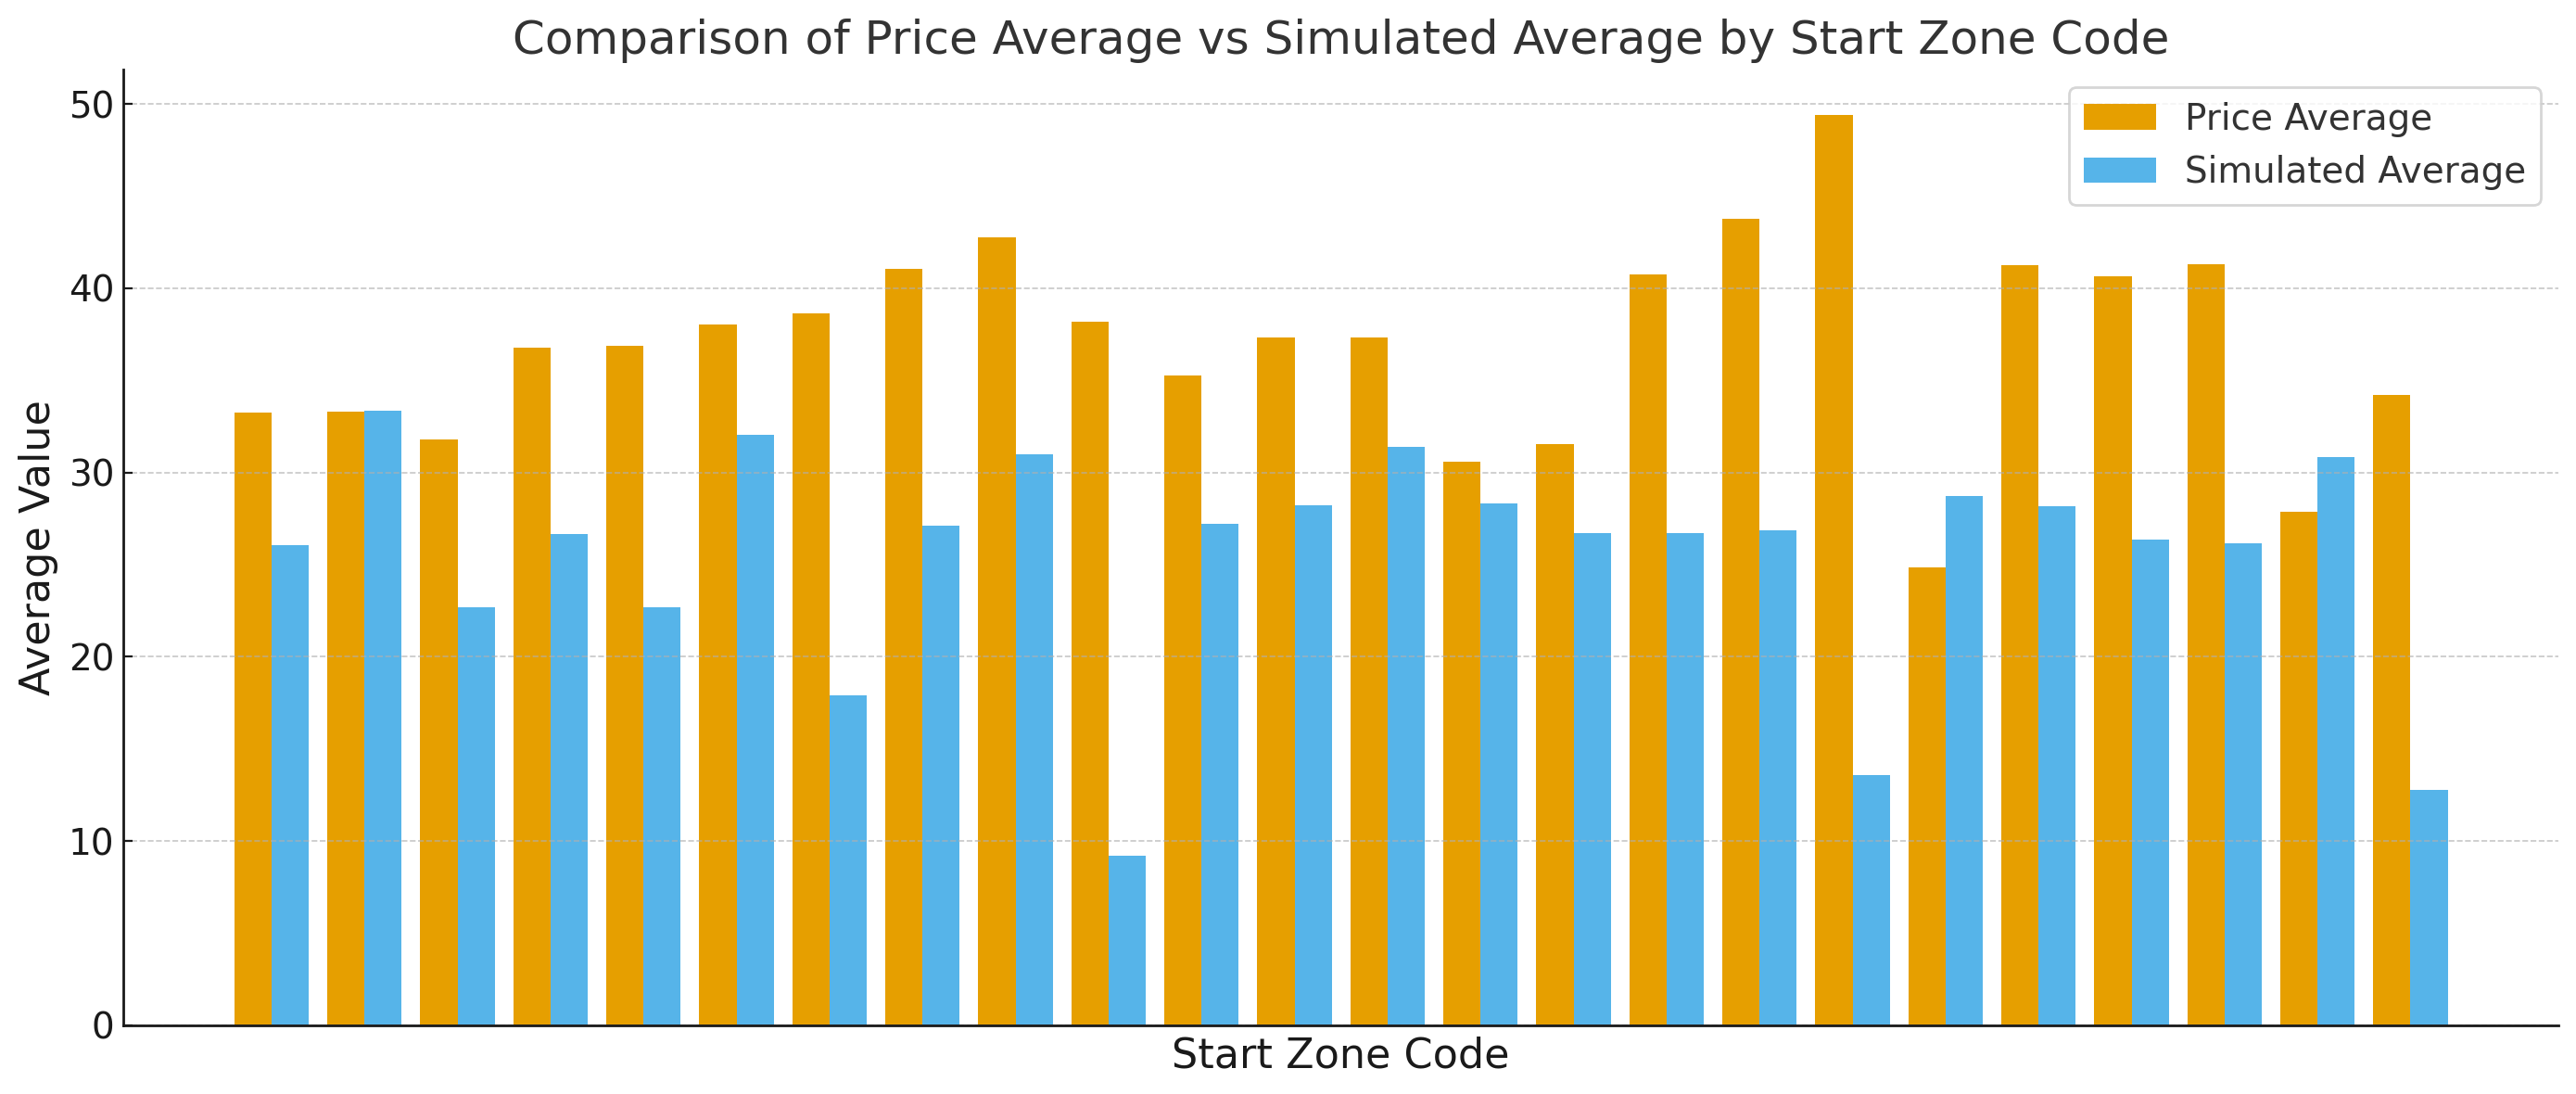
\includegraphics[width=0.5\linewidth]{images/PriceVsSimulatedPrice.png}
    \caption{Model Fit for the Short-run.}
    \label{fig:ModelFit}
\end{figure}

\begin{figure}
    \centering
    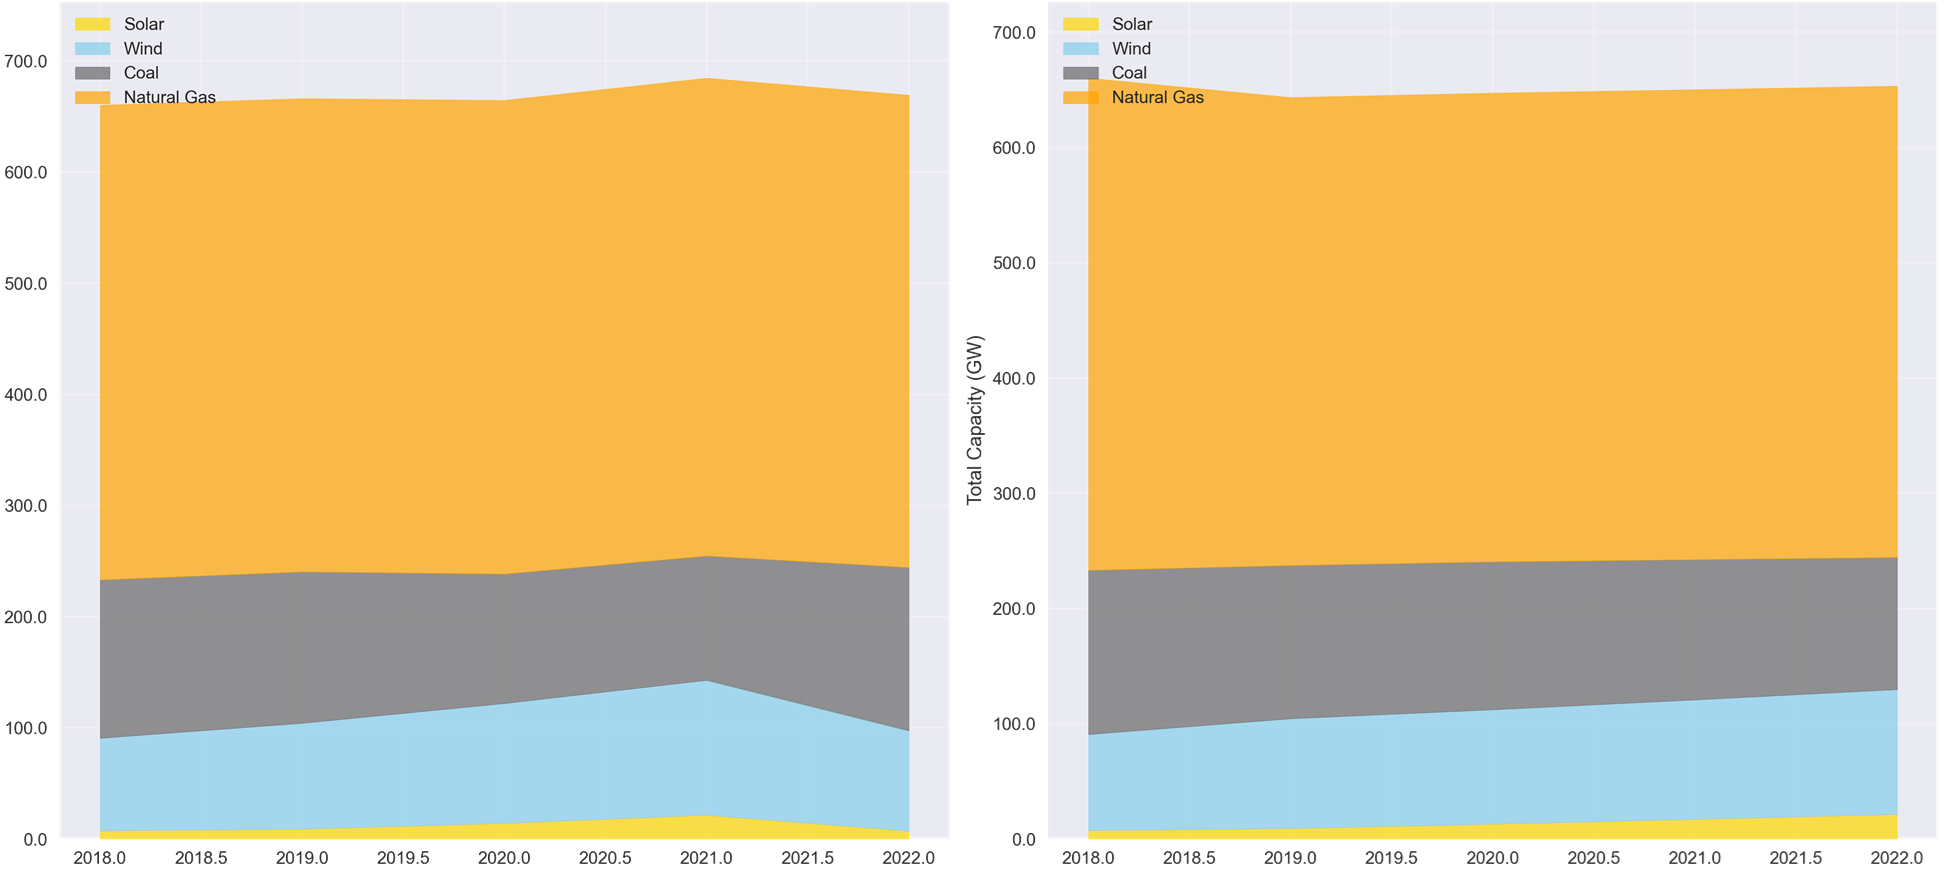
\includegraphics[width=0.5\linewidth]{images/capacity_stacked_area_Baseline.png}
    \caption{Model Fit for the Long-run.}
    \label{fig:longrunModelFit}
\end{figure}

\subsection{Robustness Checks}

I perform a suite of robustness checks detailed in Appendix Section \ref{app:robustness} and summarized in Table \ref{tab:robustness_summary}. I show the sensitivity of my a relaxation of assumptions. In particular, I show the robustness of my estimates to the allowance of blackouts and market power, varying assumptions about demand and its structure, changes to the specific dataset structure, and changes to other specific model features. The evidence presented is relatively compelling that the results are robust under slight relaxation. Some changes like market power have more impact on the estimated impacts as the level of deviation from the baseline assumption rises.

\section{Counterfactuals} \label{sec:Counterfactuals}

I use the estimated model to evaluate three sets of policy counterfactuals: upgrades to existing transmission infrastructure, addition of new long-distance transmission lines, and active federal legislation affecting both transmission and generation investment. In all counterfactual exercises, I hold estimated parameters fixed and modify only the primitives of the model---entry costs, line capacities, and per-MWh revenue---during simulation. This ensures that behavioral responses (investment, retirement, and dispatch) emerge endogenously from the estimated model rather than from re-fitting. The full set of counterfactuals run is described in Table \ref{tab:counterfactualRuns} and Figure \ref{fig:CounterfactualSimulations}.

\subsection{Transmission Infrastructure Upgrades}

The first set of counterfactuals examines the effects of upgrading existing transmission lines to High-Voltage Direct Current (HVDC) technology, which reduces line losses and increases transfer capacity. I simulate outcomes under full replacement of all inter-zonal lines as well as partial replacement of randomly selected lines at varying intensities.

Table \ref{tab:upgradeResults} reports the price impacts of transmission upgrades. Full replacement of all lines with HVDC technology reduces average wholesale prices by 6\% across the study region, generating welfare gains of approximately \$4 billion per year. This figure represents roughly one-third of total congestion costs estimated by Grid Strategies for the region. Notably, most of these gains can be achieved with partial upgrades: replacing 50\% of transmission lines still delivers price reductions exceeding 5\%.

Figure \ref{priceDecrease} illustrates how price reductions scale with the percentage of lines upgraded. The relationship exhibits diminishing returns, with the marginal benefit of additional upgrades declining as congestion on the most constrained corridors is relieved.

The effects of transmission upgrades vary substantially by region. The Northeast, where congestion costs are highest and renewable resources are scarce, experiences the largest price declines. The Midwest---home to abundant wind resources that are often curtailed due to transmission constraints---sees modest price increases as expanded export capacity raises local prices toward the national average. This price convergence, while increasing costs for some Midwestern consumers, reflects more efficient allocation of generation resources and reduced curtailment of low-cost renewable energy.

\begin{figure}
    \centering
    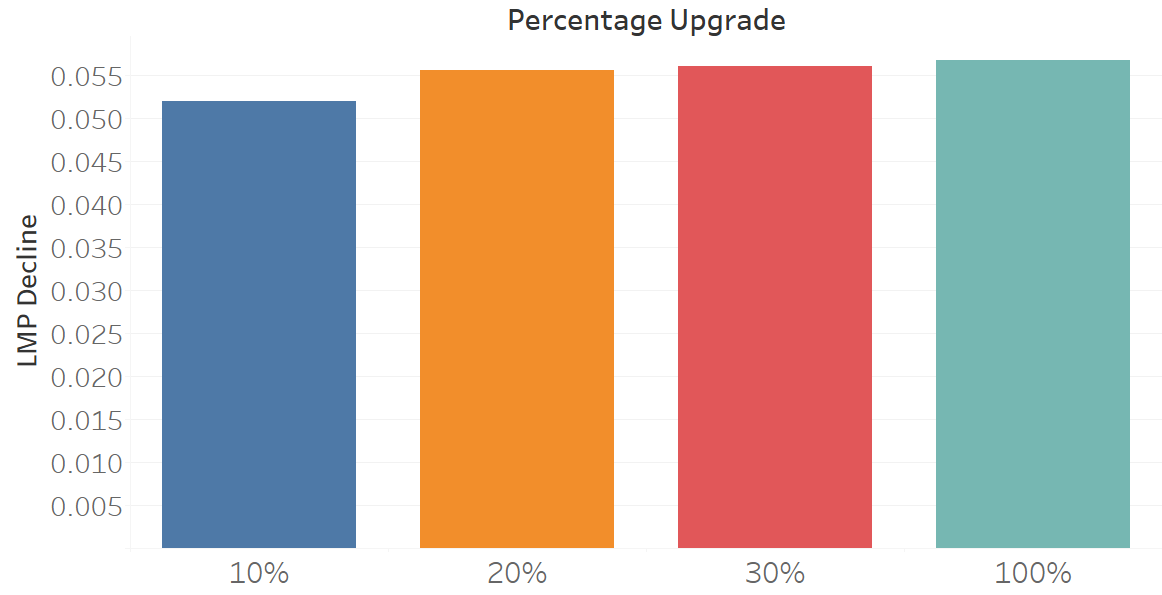
\includegraphics[width=1\linewidth]{images/LMP Decline by Percentage Upgrade.png}
    \caption{Price Decrease by Percentage Grid Upgrade}
    \label{priceDecrease}
\end{figure}

\subsection{New Long-Distance Transmission}

The second set of counterfactuals examines the addition of specific long-distance transmission projects. I first consider the limiting case of removing all transmission constraints, then evaluate specific proposed lines.

\subsubsection{Removal of All Transmission Constraints}

Eliminating all transmission constraints reduces average prices in every ISO except SPP and MISO, where prices increase as these regions become net exporters. This counterfactual also dramatically accelerates the renewable energy transition in the long-run model, as generators in renewables-rich regions can access distant markets without congestion-related price discounts.

%[PLACEHOLDER: Add specific price changes by ISO and renewable adoption numbers]

\subsubsection{Grain Belt Express}

The Grain Belt Express is a proposed 800-mile HVDC transmission line designed to carry 5,000 MW of wind power from western Kansas to Indiana and points east. In the long-run counterfactual, adding this line increases solar and wind adoption in the Eastern Interconnection by over 10\% by 2050, with the largest increases concentrated in SPP and western MISO where the line originates. 

%[PLACEHOLDER: Add additional results on prices and welfare]

\subsubsection{ERCOT-Eastern Interconnection Connection}

A major HVDC connection between ERCOT and the Eastern Interconnection would allow Texas's abundant wind and solar resources to serve load in the Southeast and beyond. 

%[PLACEHOLDER: Add description and results for the ERCOT interconnection counterfactual]

\subsection{Federal Legislation}

The final set of counterfactuals evaluates three pieces of federal legislation affecting electricity markets. These counterfactuals and their relationships are described in Table \ref{tab:factorialDesign}. I implement these policies as \textit{policy wedges}---time-varying modifications to model primitives that activate at each policy's enactment date while holding all estimated parameters fixed. This approach isolates the causal effect of each policy from the underlying structural relationships estimated from pre-policy data. To ensure comparability across scenarios, I use identical random seeds and shock draws for all simulations, so that differences across scenarios reflect only the policy treatment and not sampling variation. I run four scenarios: (i) both policies as enacted, (ii) IRA only, (iii) BIL only, and (iv) neither policy (the baseline).

\subsubsection{Big Wires Act}

The BIG WIRES Act (S.2827, 118th Congress) would mandate that each FERC Order No.\ 1000 transmission planning region achieve a Minimum Interregional Transfer Capacity (MITC) equal to at least 30\% of its coincident peak electrical demand, or an increase of 15\% over current capacity, whichever is lower, by 2035 as decribed in \cite{hickenlooper2023s}. The legislation is motivated by the widening gap between planned interregional transmission builds and anticipated need documented in the DOE's \cite{DOENationalTransmissionNeedsStudy}, driven by barriers including insufficient coordination across planning regions, cost allocation disputes, and local opposition \cite{joskow2021facilitating, pfeifenberger2021transmission}.

I follow the modeling approach of \cite{botterud2024evaluating}, who evaluate the BIG WIRES Act using the GenX capacity expansion model across 64 zones aggregated into 12 model regions that approximate the FERC Order No.\ 1000 planning regions. Their framework distinguishes interregional transmission (built between zones in different planning regions) from intraregional transmission (built within a region), and assumes that absent the Act, no new interregional transmission is built---reflecting the observed tendency of Balancing Authorities to prioritize investment within their own planning region. Under the Act, interregional capacity is expanded until each region satisfies the MITC requirement, with GenX determining the least-cost allocation of new capacity across corridors.

To implement this counterfactual in my model, I add inter-zonal transfer capacity consistent with the corridor-level builds reported in \cite{botterud2024evaluating}. I model the MITC requirement as time-varying capacity additions that phase in via a ramp function:
\begin{equation}
    A_{ij,t}^{\text{MITC}} = A_{ij,t}^{\text{baseline}} + \Delta A^{\text{MITC}}_{ij} \cdot \rho(t; t_0^{\text{MITC}}, R)
\end{equation}
where $\Delta A^{\text{MITC}}_{ij}$ is the additional transfer capacity on corridor $(i,j)$ required to satisfy the MITC constraint, calibrated to be consistent with the corridor-level estimates in \cite{botterud2024evaluating}. The largest capacity additions are concentrated in the Eastern Interconnection: between the Midwest and Mid-Atlantic, Southeast and Florida, Mid-Atlantic and Carolinas, Midwest and Central, and Mid-Atlantic and Southeast, which together account for approximately 80\% of total new interregional transmission builds under the Act.

%[PLACEHOLDER: Add specific corridor-level capacity additions used in model, mapping from Botterud et al. Table 1 to model zones, and results for prices, investment, emissions, and reliability]

\subsubsection{Inflation Reduction Act}

The Inflation Reduction Act (IRA) provides substantial tax credits for renewable energy investment, effectively reducing entry costs for solar and wind generators. I model the IRA through two channels that enter the simulation as policy wedges on the estimated model's primitives.

First, the IRA reduces entry costs for eligible renewable technologies. I implement this as a proportional reduction in the entry cost $E_k$ for eligible technology $k$:
\begin{equation}
    E_{k,t}^{\text{IRA}} = E_{k,t}^{\text{baseline}} \cdot (1 - \tau^{\text{IRA}}_k \cdot \rho(t; t_0, R))
\end{equation}
where $\tau^{\text{IRA}}_k \in [0,1)$ is the technology-specific cost reduction implied by the investment tax credit, $t_0$ is the IRA enactment date (August 2022, implemented as the first full period on or after enactment), and $\rho(t; t_0, R)$ is a ramp function that phases the credit in over $R$ periods to avoid discontinuities in the investment decision. I set $R$ to one year as a conservative default.

Second, the IRA production tax credit provides an ongoing per-MWh subsidy to eligible generators, which I model as a revenue shifter:
\begin{equation}
    P_{k,t}^{\text{eff}} = P_t + s^{\text{IRA}}_k \cdot \rho(t; t_0, R)
\end{equation}
where $s^{\text{IRA}}_k \geq 0$ is the production credit value in the same per-MWh units as the model's prices. This enters the generator's per-period profit function, raising effective revenue for eligible resources without altering the ISO's dispatch problem or the structure of the Bellman equation. Retirement decisions respond endogenously to the changed profit environment.

Eligibility is determined by a mapping from technology type to IRA-eligible status. In the baseline implementation, eligibility depends on technology $k$ alone and does not vary by region, though the framework accommodates region-specific eligibility if needed.

%[PLACEHOLDER: Add specific values of tau_IRA and s_IRA by technology, and results for renewable adoption, prices, and emissions]

\subsubsection{Bipartisan Infrastructure Law}

The Bipartisan Infrastructure Law (BIL) provides funding for transmission infrastructure including grants for interregional transmission projects. I model the BIL as a time-varying expansion of inter-zonal transfer capacities:
\begin{equation}
    A_{ij,t}^{\text{BIL}} = A_{ij,t}^{\text{baseline}} + \Delta A^{\text{BIL}}_{ij} \cdot \rho(t; t_0^{\text{BIL}}, R)
\end{equation}
where $\Delta A^{\text{BIL}}_{ij} \geq 0$ represents the additional transfer capacity on corridor $(i,j)$ funded by the BIL, in the same units as the baseline line limits $A_{ij}$, and $t_0^{\text{BIL}}$ is the BIL enactment date (November 2021). The adjusted capacities enter the ISO dispatch problem's constraint set, expanding the feasible region for inter-zonal power flows. The dispatch objective and optimality conditions are otherwise unchanged.

I consider two specifications for the BIL transmission expansion. The first is corridor-specific, assigning $\Delta A^{\text{BIL}}_{ij}$ values to individual lines consistent with announced project funding. The second is a system-wide specification in which each corridor receives a proportional expansion $\Delta A^{\text{BIL}}_{ij} = \alpha \cdot A_{ij,t}^{\text{baseline}}$, parameterized by a single scalar $\alpha > 0$.

%[PLACEHOLDER: Add specific corridor expansions or alpha value, and results]

\subsubsection{Combined Policy Effects}

Running these policies in combination reveals whether transmission investment and renewable subsidies act as substitutes or complements. Formally, I compare the welfare gain from the joint policy $\Delta W^{\text{IRA+BIL}} = W^{\text{as\_enacted}} - W^{\text{no\_ira\_no\_bil}}$ against the sum of individual effects $\Delta W^{\text{IRA}} + \Delta W^{\text{BIL}}$, where $\Delta W^{\text{IRA}} = W^{\text{no\_bil}} - W^{\text{no\_ira\_no\_bil}}$ and $\Delta W^{\text{BIL}} = W^{\text{no\_ira}} - W^{\text{no\_ira\_no\_bil}}$. Complementarity implies $\Delta W^{\text{IRA+BIL}} > \Delta W^{\text{IRA}} + \Delta W^{\text{BIL}}$.

The results indicate that these policies are largely complementary: renewable subsidies increase the supply of low-cost generation, while transmission investment ensures this generation can reach high-demand markets. The mechanism is intuitive---the IRA lowers entry costs, inducing additional renewable capacity in resource-rich regions, but the value of this capacity is limited by transmission constraints that prevent it from reaching high-price markets. The BIL relaxes these constraints, raising the effective price received by new entrants and amplifying the IRA's investment incentive. Implementing both policies together yields welfare gains exceeding the sum of individual effects, suggesting that a portfolio approach to energy transition policy dominates single-instrument strategies. I include estimates of the costs of the policies and show that all are welfare improving even after considering costs.

%[PLACEHOLDER: Add combined results with specific numbers]

\subsection{Welfare Decomposition}

I run a welfare decomposition where I demonstrate how gains accrue to producers and consumers at the zonal level. While the total system-wide surplus is obviously positive for both producers and consumers, the distribution of the surplus is significantly varied. In some regions, mainly ERCOT and specific zones within PJM, welfare is uniformly improved. This occurs because the insurance effect dominates with producers exporting more electricity during low-cost hours and importing during high-cost hours. For regions with significant renewable energy and low prices before transmission expansion, producer welfare increases while consumer welfare decreases. The opposite occurs in regions with fewer renewable resources and higher initial prices. I quantify these effects and provide useful intuition for policy-makers as to what transfers could be made to make the policy Pareto-improving.

\section{Conclusion} \label{sec:conclusion}

This paper develops and estimates a dynamic model of generator behavior in electricity markets with transmission constraints, linking short-run dispatch decisions to long-run capacity investment. The model captures how transmission infrastructure shapes price formation across interconnected markets and how these prices influence firms' incentives to invest in different generation technologies.

Three main findings emerge from the analysis. First, transmission constraints impose substantial costs on electricity consumers: upgrading existing infrastructure to modern HVDC standards would reduce wholesale prices by 6\% and generate \$4 billion in annual welfare gains. Second, the benefits of transmission investment are regionally heterogeneous, with the largest gains accruing to transmission-constrained regions in the Northeast. Third, in the long run, expanded transmission capacity accelerates the renewable energy transition by allowing generators in renewables-rich regions to access distant markets, increasing solar and wind adoption by over 10\% by 2050 under scenarios including major projects like the Grain Belt Express.

The policy counterfactuals indicate that transmission investment and renewable energy subsidies act as complements rather than substitutes. Policies like the Inflation Reduction Act increase the supply of renewable generation, while transmission investments under the Bipartisan Infrastructure Law and Big Wires Act ensure this generation can reach consumers. Implementing both types of policies together yields benefits exceeding the sum of their individual effects.

Several limitations suggest directions for future research. The model operates at the zonal rather than nodal level, preventing analysis of specific substation-to-substation connections. This limitation makes the model better suited to evaluating large-scale interregional transmission than individual line additions. Additionally, the model treats demand as exogenous; long-run shifts in the geographic distribution of load in response to electricity price changes represent an important extension. Finally, the model does not incorporate storage, which may interact with transmission as alternative solutions to renewable intermittency.

Despite these limitations, the results provide evidence that transmission investment offers a cost-effective complement to direct renewable subsidies in accelerating the energy transition. As policymakers evaluate proposals to expand interregional transmission capacity, models that capture both the short-run operational benefits and long-run investment effects can inform the efficient allocation of infrastructure spending.

\pagebreak

\singlespacing
\setlength\bibsep{0pt}
\printbibliography




\clearpage

\onehalfspacing

\section*{Tables} \label{sec:tab}
\addcontentsline{toc}{section}{Tables}

\begin{table}[htbp]
\centering
\begin{tabular}{lcccc}
\toprule
\textbf{ISO} & \textbf{Mean Price} & \textbf{Mean Load} & \textbf{Median Price} & \textbf{Median Load} \\
\midrule
ISO-NE & 50 & 13{,}623 & 45 & 13{,}308 \\
%IESO   & 20 & 16{,}140 & 11 & 15{,}283 \\
NYISO  & 43 & 17{,}686 & 39 & 17{,}297 \\
ERCOT  & 40 & 44{,}328 & 23 & 41{,}901 \\
%CAISO  & 46 & 25{,}477 & 39 & 24{,}585 \\
SPP    & 37 & 30{,}420 & 30 & 29{,}246 \\
MISO   & 38 & 73{,}945 & 34 & 72{,}179 \\
PJM    & 41 & 146{,}112 & 37 & 88{,}236 \\
\bottomrule
\end{tabular}
\caption{Average and Median Price and Load by ISO}
\label{priceData}
\end{table}

\begin{table}[htbp]
\centering
\begin{tabular}{lccc}
\toprule
\textbf{Variable} & \textbf{Mean} & \textbf{Standard Deviation} & \textbf{Median} \\
\midrule
Load & 5{,}075 & 7{,}055 & 2{,}296 \\
Price & 37.8 & 79.5 & 27.6 \\
SO\textsubscript{2} Emissions & 526 & 417 & 470 \\
Solar Generation & 2 & 13 & 0.03 \\
Wind Generation & 44 & 61 & 20 \\
Natural Gas Generation & 29 & 66 & 33 \\
Coal Generation & 162 & 217 & 64 \\
Exports & 18.9 & 76.3 & 0.53 \\
\bottomrule
\end{tabular}
\caption{Descriptive Statistics: Short-run}
\label{ShortTermStats1}
\end{table}

\begin{table}[htbp]
\centering
\begin{tabular}{lccc}
\toprule
\textbf{Variable} & \textbf{Mean} & \textbf{Standard Deviation} & \textbf{Median} \\
\midrule
Fuel Cost & 603 & 2{,}093 & 324 \\
Heat Content & 3.6 & 6.0 & 1.03 \\
Natural Gas Spot Price & 3.8 & 2.3 & 2.7 \\
%Natural Gas Futures Price & 3.8 & 2.1 & 2.7 \\
Coal Spot Price & 166 & 128 & 98 \\
Temperature & 13 & 12 & 15 \\
Loss Percentage & 0.05 & 0.06 & 0.05 \\
Transmission Constraint & 0.51 & 1.00 & 0.50 \\
Capacity Constraint & 0.06 & 66 & 33 \\
\bottomrule
\end{tabular}
\caption{Descriptive Statistics: Short-run}
\label{ShortTermStats2}
\end{table}

\begin{table}[htbp]
\centering
\begin{tabular}{lcccc}
\toprule
\textbf{Resource} & \textbf{Intercept} & \textbf{Signif.} & \textbf{Export Coeff.} & \textbf{Signif.} \\
\midrule
Electricity used for energy storage & 30.97 & *** & 0.02 & *** \\
Natural Gas                         & 37.72& *** & 0.01 &  ***\\
Nuclear (incl. Uranium, Plutonium, Thorium) & 46.44 & *** & 0.01 & *** \\
Coal                                & 30.97 & *** & 32.47 & *** \\
Distillate Fuel Oil (diesel, No.\,1--4) & 33.23 &  *** & 0.01 & *** \\
Landfill Gas                        & 33.91 & *** & 0.00 & *** \\
Water at hydro or hydrokinetic technologies & 36.27 & *** & -0.02 & *** \\
Other Biomass Gas (digester, methane, etc.) & 27.64 & *** & -0.11 & *** \\
Petroleum Coke                      & 31.50 & *** & 0.06 &  ***\\
Wood/Wood Waste Solids              & 40.91 &  ***& 0.06 &  ***\\
Blast Furnace Gas                   & 30.34 & *** & 0.00 &  ***\\
Waste heat (no direct fuel source) & 37.43 & *** & 0.01 &  ***\\
Black Liquor                        & 30.97 & *** & 0.01 & *** \\
Other Gas                           & 41.99 & *** & -0.12 & *** \\
Other                               & 30.97 & *** & 0.10 & *** \\
Purchased Steam                     & 30.97 & *** & -0.02 & *** \\
Agricultural By-Products            & 29.56 & *** & -0.06 &  ***\\
Petroleum Products                  & 34.94 & *** & 0.00 & *** \\
\bottomrule
\end{tabular}
\vspace{0.5em}

\footnotesize\textit{Note:} Export coefficients represent the marginal relationship between exports and output by energy resource. Significance codes: *** $p<0.01$, ** $p<0.05$, * $p<0.1$. The log-likelihood of the regression is 7.662301.
\caption{Short-run Model Estimates by Resource Type}
\label{ResourcesTable}
\end{table}

\begin{table}[htbp]
\centering
\begin{tabular}{lcc}
\toprule
\textbf{Variable} & \textbf{Estimate} & \textbf{Significance} \\
\midrule
Natural Gas Price & 6.93 & *** \\
Dewpoint               & 2.46 & *** \\
Temperature            & 0.00 &     \\
Heat Content              & -2.22& *** \\
Generator Startup              & -2.3& *** \\
 Generator Near Capacity             & -2.3& *** \\
\bottomrule
\end{tabular}
\vspace{0.5em}

\footnotesize\textit{Notes:} Specification includes hourly and monthly dummies, zone-code dummies, and severe weather dummies.
\caption{Estimates for Natural Gas Covariates}
\label{NaturalGasTable}
\end{table}

\begin{table}[htbp]
\centering
\begin{tabular}{lcc}
\toprule
\textbf{Variable} & \textbf{Estimate} & \textbf{Significance} \\
\midrule
Coal Price     & 8.68  & *** \\
Dewpoint       & 2.46  & *** \\
Temperature    & 4.00  & *** \\
Heat Rate      & -1.30 & *** \\
Generator Startup              & -2.3& *** \\
 Generator Near Capacity             & -2.3& *** \\
\bottomrule
\end{tabular}
\vspace{0.5em}

\footnotesize\textit{Notes:} Specification includes hourly and monthly dummies, zone-code dummies, and severe weather dummies.
\caption{Estimates for Coal Covariates}
\label{CoalTable}
\end{table}

% ============================================================
% Table 1: Master table of all counterfactual runs
% ============================================================

\begin{landscape}
    \begin{table}[htbp]
        \centering
        \caption{Counterfactual Simulation Scenarios}
        \label{tab:counterfactualRuns}
        \small 
        % Defines columns: 
        % 1: Left align (Scenario)
        % 2: Paragraph 5cm (Description)
        % 3-5: Centered paragraph 2.5cm (The checkmark columns)
        \begin{tabular}{@{} l p{5cm} >{\centering\arraybackslash}p{2.5cm} >{\centering\arraybackslash}p{2.5cm} >{\centering\arraybackslash}p{2.5cm} @{}}
            \toprule
            & & \multicolumn{3}{c}{\textit{Modified Primitives}} \\
            \cmidrule(lr){3-5}
            \textbf{Scenario} & \textbf{Description} & Line Capacity \newline $A_{ij}$ & Entry Cost \newline $E_k$ & Revenue \newline $P_k^{\text{eff}}$ \\
            \midrule
            
            % --- PANEL A ---
            \multicolumn{5}{l}{\textit{Panel A: Transmission Infrastructure Upgrades}} \\[0.5ex]
            Full HVDC & All inter-zonal lines replaced with HVDC & $\checkmark$ & & \\
            Partial HVDC & Random subset at intensity $\alpha \in (0,1)$ & $\checkmark$ & & \\[1.5ex]
            
            % --- PANEL B ---
            \multicolumn{5}{l}{\textit{Panel B: New Long-Distance Transmission}} \\[0.5ex]
            No constraints & All transmission limits removed & $\checkmark$ & & \\
            Grain Belt Express & 5,000~MW HVDC, KS to IN & $\checkmark$ & & \\
            ERCOT--Eastern IC & HVDC link, ERCOT to Southeast & $\checkmark$ & & \\[1.5ex]
            
            % --- PANEL C ---
            \multicolumn{5}{l}{\textit{Panel C: Federal Legislation}} \\[0.5ex]
            BIG WIRES Act & MITC $\geq$ 30\% peak demand by 2035 & $\checkmark$ & & \\[1.5ex]
            
            \multicolumn{5}{l}{\quad\textit{IRA $\times$ BIL Factorial Design}} \\[0.5ex]
            Baseline & Neither IRA nor BIL & & & \\
            IRA only & IRA enacted, no BIL & & $\checkmark$ & $\checkmark$ \\
            BIL only & BIL enacted, no IRA & $\checkmark$ & & \\
            As enacted & Both IRA and BIL & $\checkmark$ & $\checkmark$ & $\checkmark$ \\[1.5ex]
            
            % --- PANEL D ---
            \multicolumn{5}{l}{\textit{Panel D: Cross-Cutting Analysis}} \\[0.5ex]
            Welfare & Producer/consumer surplus & \multicolumn{3}{c}{\textit{Applied to all scenarios}} \\
            decomposition & by zone for each scenario & \multicolumn{3}{c}{} \\
            \bottomrule
        \end{tabular}
        
        % Table Notes (Placed simply below the tabular)
        \vspace{1ex}
        \begin{minipage}{\linewidth}
            \footnotesize
            \textit{Notes:} Each scenario holds estimated structural parameters fixed and modifies only the indicated model primitives. $A_{ij}$ denotes inter-zonal transfer capacity, $E_k$ denotes technology-specific entry cost, and $P_k^{\text{eff}}$ denotes effective per-MWh revenue inclusive of production tax credits. All policy wedges phase in via a ramp function $\rho(t; t_0, R)$ to avoid discontinuities. Panel~C scenarios use identical random seeds and shock draws to isolate policy effects from sampling variation.
        \end{minipage}
    \end{table}
\end{landscape}

%\vspace{1.5cm}

% ============================================================
% Table 2: Federal legislation factorial design and
%          complementarity comparisons
% ============================================================

\begin{table}[htbp]
\centering
\begin{threeparttable}
\caption{Federal Legislation: Factorial Design and Complementarity Test}
\label{tab:factorialDesign}
\small
\begin{tabular}{@{} l cc @{}}
\toprule
& \multicolumn{2}{c}{\textbf{Bipartisan Infrastructure Law}} \\
\cmidrule(lr){2-3}
\textbf{Inflation Reduction Act} & Not enacted & Enacted \\
\midrule
Not enacted & $W^{\text{baseline}}$ & $W^{\text{BIL only}}$ \\[10pt]
Enacted & $W^{\text{IRA only}}$ & $W^{\text{as enacted}}$ \\
\bottomrule
\end{tabular}

\vspace{0.6cm}

\begin{tabular}{@{} L{4.2cm} l @{}}
\toprule
\textbf{Comparison} & \textbf{Definition} \\
\midrule
IRA marginal effect & $\Delta W^{\text{IRA}} = W^{\text{IRA only}} - W^{\text{baseline}}$ \\[4pt]
BIL marginal effect & $\Delta W^{\text{BIL}} = W^{\text{BIL only}} - W^{\text{baseline}}$ \\[4pt]
Joint effect & $\Delta W^{\text{joint}} = W^{\text{as enacted}} - W^{\text{baseline}}$ \\[4pt]
Complementarity & $\Delta W^{\text{joint}} - \bigl(\Delta W^{\text{IRA}} + \Delta W^{\text{BIL}}\bigr) > 0$ \\
\bottomrule
\end{tabular}

\begin{tablenotes}[flushleft]
\footnotesize
\item \textit{Notes:} $W$ denotes total welfare (consumer plus producer surplus). The top panel displays the $2 \times 2$ factorial structure of the federal legislation counterfactuals. The bottom panel defines the comparisons used to test policy complementarity. Complementarity holds when the joint welfare gain exceeds the sum of individual gains, indicating that transmission investment (BIL) and renewable subsidies (IRA) are mutually reinforcing.
\end{tablenotes}
\end{threeparttable}
\end{table}

% \begin{table}[ht]
% \centering
% \caption{Resource-Specific Parameter Estimates}
% \begin{threeparttable}
% \resizebox{\textwidth}{!}{%
% \begin{tabular}{l*{8}{c}}
% \toprule
% \textbf{Resource Type} & $F_0$ & $E_0$ & $\rho_{1k}$ & $\rho_{2k}$ & $\psi_{1k}$ & $\sigma^2_{\zeta_1}$ & $\sigma^2_{\zeta_2}$ & $\psi_{2k}$ \\
%  & (s.e.) & (s.e.) & (s.e.) & (s.e.) & (s.e.) & (s.e.) & (s.e.) & (s.e.) \\
% \midrule
% Coal         & -0.080 &  0.160 & -0.151 &  0.019 & -0.015 & 0.127 &  0.055 & -0.106 \\
%              & [PLACEHOLDER] & [PLACEHOLDER] & [PLACEHOLDER] & [PLACEHOLDER] & [PLACEHOLDER] & [PLACEHOLDER] & [PLACEHOLDER] & [PLACEHOLDER] \\
% Natural Gas  & -0.242 & -0.116 & -0.076 &  0.058 &  0.140 & 0.155 &  0.172 &  0.128 \\
%              & [PLACEHOLDER] & [PLACEHOLDER] & [PLACEHOLDER] & [PLACEHOLDER] & [PLACEHOLDER] & [PLACEHOLDER] & [PLACEHOLDER] & [PLACEHOLDER] \\
% Solar        &  0.091 &  0.018 & -0.115 &  0.072 &  0.102 & 0.048 & 0.085 &  0.017 \\
%              & [PLACEHOLDER] & [PLACEHOLDER] & [PLACEHOLDER] & [PLACEHOLDER] & [PLACEHOLDER] & [PLACEHOLDER] & [PLACEHOLDER] & [PLACEHOLDER] \\
% Wind         &  0.276 & -0.007 & -0.081 &  0.223 & -0.191 & 0.027 & 0.142 &  0.095 \\
%              & [PLACEHOLDER] & [PLACEHOLDER] & [PLACEHOLDER] & [PLACEHOLDER] & [PLACEHOLDER] & [PLACEHOLDER] & [PLACEHOLDER] & [PLACEHOLDER] \\
% \bottomrule
% \end{tabular}
% }
% \begin{tablenotes}
% \small
% \item \textit{Notes:} Standard errors in brackets. [PLACEHOLDER: Add note on estimation method for standard errors]
% \end{tablenotes}
% \end{threeparttable}
% \label{longRunResults}
% \end{table}

% \begin{table}[htbp]
% \centering
% \caption{Price Impacts of Transmission Upgrades}
% \begin{tabular}{lcccc}
% \toprule
% \textbf{Upgrade Percentage} & \textbf{Avg. Price Change} & \textbf{Welfare Gain (\$/yr)} & \textbf{NE Change} & \textbf{MW Change} \\
% \midrule
% 25\% & [PLACEHOLDER] & [PLACEHOLDER] & [PLACEHOLDER] & [PLACEHOLDER] \\
% 50\% & $>$5\% reduction & [PLACEHOLDER] & [PLACEHOLDER] & [PLACEHOLDER] \\
% 75\% & [PLACEHOLDER] & [PLACEHOLDER] & [PLACEHOLDER] & [PLACEHOLDER] \\
% 100\% & 6\% reduction & \$4 billion & Largest decline & Modest increase \\
% \bottomrule
% \end{tabular}
% \label{tab:upgradeResults}
% \end{table}

\clearpage

\section*{Figures} \label{sec:fig}
\addcontentsline{toc}{section}{Figures}

% \begin{center}
% \begin{figure}
% \begin{tikzpicture}[node distance=2cm, every node/.style={align=center, font=\small}, scale=.45, transform shape]

%     % Supply Nodes with Labels above the boxes
%     \node (supply1_label) [above=0.2cm] at (0,0) {Supply Node $j$};
%     \node (supply1) [draw, rectangle, minimum width=3cm, minimum height=5cm, below=0.2cm of supply1_label] {};

%     \node (supply2_label) [above=0.2cm, right=6cm of supply1_label] {Supply Node $j'$};
%     \node (supply2) [draw, rectangle, minimum width=3cm, minimum height=5cm, below=0.2cm of supply2_label] {};

%     % Generators at Supply Node j
%     \node (gen1) [draw, rectangle, below=0.8cm of supply1.north, minimum width=2.5cm] {Generator $G$};
%     \node (gen1_label) [left=0.5cm of gen1] {Marginal Resource};

%     \node (gen2) [draw, rectangle, below=0.8cm of gen1, minimum width=2.5cm] {Generator $G'$};
%     \node (gen2_label) [left=0.5cm of gen2] {Capacity Constrained};

%     % Generators at Supply Node j'
%     \node (gen3) [draw, rectangle, below=0.8cm of supply2.north, minimum width=2.5cm] {Generator $G$};
%     \node (gen3_label) [right=0.5cm of gen3] {Marginal Resource};

%     \node (gen4) [draw, rectangle, below=0.8cm of gen3, minimum width=2.5cm] {Generator $G'$};
%     \node (gen4_label) [right=0.5cm of gen4] {};

%     % Demand Nodes
%     \node (demand1) [draw, circle, minimum width=1cm, below=4cm of supply1, label=below:{Demand Node $i$}] {Demand Node $i$, $L_i,LMP_i$};
%     \node (demand2) [draw, circle, minimum width=1cm, below=4cm of supply2, label=below:{Demand Node $i'$}] {Demand Node $i'$, $L_i',LMP_i'$};

%     % Arrows from Supply Nodes to Demand Nodes with Labels
%     \draw[-{Stealth}, thick] (supply1.south) to [out=-135, in=135, looseness=1.5] (demand1.north) node[midway, left, xshift=-0.3cm] {};
%     \draw[-{Stealth}, thick, dashed] (supply1.south) to [out=-45, in=135, looseness=1.2] (demand2.north) node[midway, above, xshift=0.5cm] {};
%     \draw[-{Stealth}, thick, dashed] (supply2.south) to [out=-135, in=45, looseness=1.2] (demand1.north east) node[midway, right, xshift=-0.3cm] {};
%     \draw[-{Stealth}, thick] (supply2.south) to [out=-45, in=45, looseness=1.5] (demand2.north) node[midway, right, xshift=-0.3cm] {};

% \end{tikzpicture}
%     \caption{Sample two-node network.}
%     \label{SampleNetwork}
% \end{figure}
% \end{center}

\begin{center}
   \begin{figure}[H]
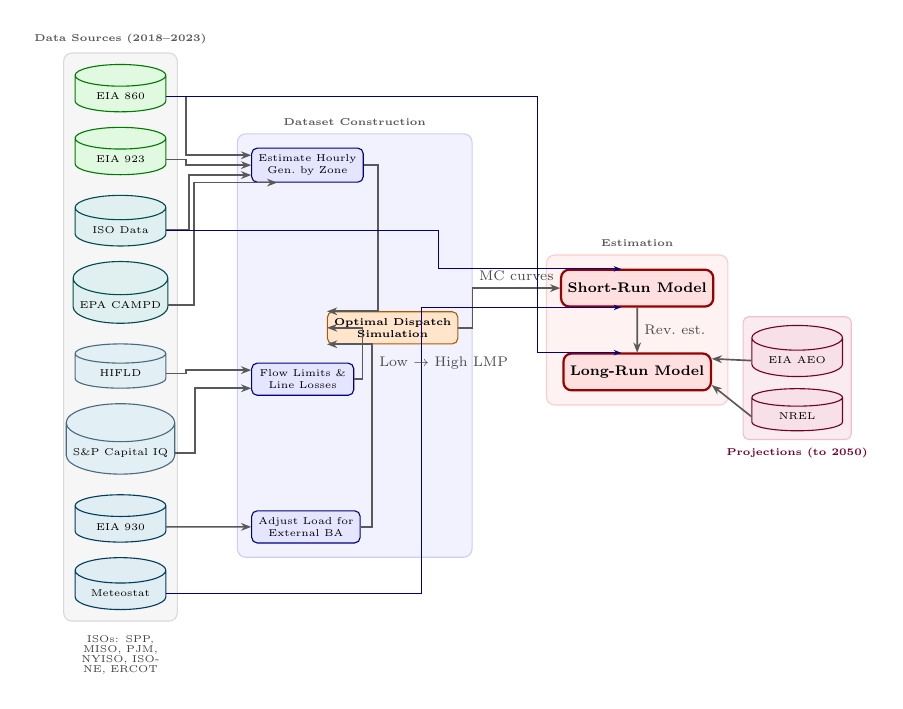
\begin{tikzpicture}[
    scale=0.72,
    transform shape,
    node distance=0.48cm and 0.7cm,
    % === STYLES ===
    source/.style={
        cylinder,
        shape border rotate=90,
        draw=#1!60!black,
        fill=#1!12,
        text centered,
        minimum height=1.55em,
        minimum width=1.6cm,
        aspect=0.35,
        font=\tiny,
        align=center
    },
    source/.default=green,
    process/.style={
        rectangle,
        draw=blue!50!black,
        fill=blue!10,
        text centered,
        rounded corners=2pt,
        minimum height=1.35em,
        minimum width=1.8cm,
        font=\tiny,
        align=center
    },
    dispatch/.style={
        rectangle,
        draw=orange!70!black,
        fill=orange!20,
        text centered,
        rounded corners=2pt,
        minimum height=1.6em,
        minimum width=1.9cm,
        font=\tiny\bfseries,
        align=center
    },
    model/.style={
        rectangle,
        draw=red!60!black,
        fill=red!12,
        thick,
        text centered,
        rounded corners=3pt,
        minimum height=1.85em,
        minimum width=2.2cm,
        font=\scriptsize\bfseries,
        align=center
    },
    arrow/.style={
        -{Stealth[scale=0.65]},
        semithick,
        color=gray!70!black
    },
    directarrow/.style={
        -{Stealth[scale=0.55]},
        color=blue!50!black,
        thin
    },
    grouplabel/.style={
        font=\tiny\bfseries,
        color=gray!70!black
    },
    annot/.style={
        font=\scriptsize,
        color=gray!60!black
    }
]

% === COLUMN 1: RAW DATA SOURCES ===

% Generator/Capacity Data (green shades)
\node[source=green!80!black] (eia860) {EIA 860};
\node[source=green!80!black, below=0.26cm of eia860] (eia923) {EIA 923};

% Real-time/Operational Data (teal shades)
\node[source=teal, below=0.35cm of eia923] (iso) {ISO Data};
\node[source=teal, below=0.26cm of iso] (campd) {EPA CAMPD};

% Grid Infrastructure (cyan shades)
\node[source=cyan!70!black, below=0.35cm of campd] (hifld) {HIFLD};
\node[source=cyan!70!black, below=0.26cm of hifld] (spiq) {S\&P Capital IQ};

% Flows and Weather (blue-green shades)
\node[source=blue!60!green, below=0.35cm of spiq] (eia930) {EIA 930};
\node[source=blue!60!green, below=0.26cm of eia930] (weather) {Meteostat};

% === COLUMN 2: DATA CONSTRUCTION STEPS ===

% Generation Estimation
\node[process, right=1.5cm of eia923, yshift=-0.1cm] (gen_est) {Estimate Hourly\\Gen.\ by Zone};

% Transmission Network
\node[process, right=1.5cm of hifld, yshift=-0.1cm] (trans_est) {Flow Limits \&\\Line Losses};

% Load Adjustment
\node[process, right=1.5cm of eia930] (load_adj) {Adjust Load for\\External BA};

% Dispatch Simulation (central step)
\node[dispatch, right=2.8cm of campd, yshift=-0.4cm] (dispatch) {Optimal Dispatch\\Simulation};

% === COLUMN 3: ESTIMATION MODELS ===

% Short-Run Model
\node[model, right=1.8cm of dispatch, yshift=0.7cm] (short_run) {Short-Run Model};

% Long-Run Model  
\node[model, below=0.8cm of short_run] (long_run) {Long-Run Model};

% Projection Sources (for Long-Run)
\node[source=purple, right=0.7cm of long_run, yshift=0.2cm] (aeo) {EIA AEO};
\node[source=purple, below=0.2cm of aeo] (nrel) {NREL};

% === CONNECTIONS ===

% To Generation Estimation
\draw[arrow] (eia860.east) -- ++(0.35,0) |- (gen_est.170);
\draw[arrow] (eia923.east) -- ++(0.35,0) |- (gen_est.west);
\draw[arrow] (iso.east) -- ++(0.4,0) |- (gen_est.190);
\draw[arrow] (campd.east) -- ++(0.45,0) |- (gen_est.210);

% To Transmission Estimation
\draw[arrow] (hifld.east) -- ++(0.35,0) |- (trans_est.170);
\draw[arrow] (spiq.east) -- ++(0.35,0) |- (trans_est.190);

% To Load Adjustment
\draw[arrow] (eia930) -- (load_adj);

% To Dispatch Simulation - arrows enter from top-left area to avoid text
\draw[arrow] (gen_est.east) -- ++(0.25,0) |- (dispatch.north west);
\draw[arrow] (trans_est.east) -- ++(0.15,0) |- (dispatch.west);
\draw[arrow] (load_adj.east) -- ++(0.2,0) |- (dispatch.south west);

% Dispatch to Short-Run Model
\draw[arrow] (dispatch.east) -- ++(0.25,0) |- node[pos=0.75, above, annot] {MC curves} (short_run.west);

% Direct feeds to Short-Run Model
\draw[directarrow] (weather.east) -- ++(4.5,0) |- (short_run.230);
\draw[directarrow] (iso.east) -- ++(4.8,0) |- (short_run.130);

% Short-Run to Long-Run
\draw[arrow] (short_run.south) -- node[midway, right, annot] {Rev.\ est.} (long_run.north);

% Projections to Long-Run
\draw[arrow] (aeo.west) -- (long_run.10);
\draw[arrow] (nrel.west) -- (long_run.350);

% EIA 860 capacity data to Long-Run
\draw[directarrow] (eia860.east) -- ++(6.55,0) |- (long_run.130);

% === BACKGROUND GROUPINGS ===
\begin{scope}[on background layer]
    % Raw Data Sources
    \node[fit=(eia860)(weather), 
          fill=gray!7, 
          rounded corners=3pt, 
          draw=gray!30,
          inner sep=4pt] (rawbox) {};
    \node[grouplabel, above=0.02cm of rawbox.north] {Data Sources (2018--2023)};
    
    % Data Construction
    \node[fit=(gen_est)(load_adj)(dispatch)(trans_est), 
          fill=blue!5, 
          rounded corners=3pt, 
          draw=blue!20,
          inner sep=5pt] (constructbox) {};
    \node[grouplabel, above=0.02cm of constructbox.north] {Dataset Construction};
    
    % Models
    \node[fit=(short_run)(long_run), 
          fill=red!5, 
          rounded corners=3pt, 
          draw=red!20,
          inner sep=5pt] (modelbox) {};
    \node[grouplabel, above=0.02cm of modelbox.north] {Estimation};
    
    % Projections
    \node[fit=(aeo)(nrel), 
          fill=purple!8, 
          rounded corners=2pt, 
          draw=purple!25,
          inner sep=3pt] (projbox) {};
    \node[grouplabel, below=0.01cm of projbox.south, color=purple!60!black] {Projections (to 2050)};
\end{scope}

% === ANNOTATIONS ===
% Position LMP annotation below dispatch box, slightly right of center to avoid arrows
\node[annot, below=0.1cm of dispatch.south, xshift=0.9cm] {Low $\to$ High LMP};

% ISO coverage note
\node[font=\fontsize{4}{5}\selectfont, color=gray!50!black, below=0.12cm of rawbox.south, text width=2.2cm, align=center] 
    {ISOs: SPP, MISO, PJM,\\NYISO, ISO-NE, ERCOT};

\end{tikzpicture}
    \caption{Dataset Construction Diagram.}
    \label{DataSetCreation}
    \end{figure}
\end{center}

% \begin{center}
%    \begin{figure}
%     \begin{tikzpicture}[scale=0.225, every node/.style={transform shape},
%         block/.style={rectangle, draw, text centered, rounded corners, minimum height=2.5em, minimum width=11em, fill=blue!10, font=\Huge},
%         arrow/.style={-{Stealth[scale=1]}, thick},
%         node distance=3cm  % Increase node distance for more space
%     ]
%         % Input Sources
%         \node[block] (iso) {ISO Data \\ (Load, Price, Fuel Mix)};
%         \node[block, below=of iso, yshift=-0.5cm] (net_exports) {Net Exports \\ (EIA)};

%         % Generation Data and Generator Data
%         \node[block, right=6cm of iso] (generation) {Generation Data};
%         \node[block, above=of generation, yshift=0.5cm] (generator) {Generator Data \\ (EIA 923, EPA CAMPD, EIA 860)};

%         % Processes
%         \node[block, below=3.5cm of generation] (line_loss) {Estimate Line Losses \& Flow Limits};
%         \node[block, below=of line_loss, yshift=-0.5cm] (load_adjust) {Adjust Load by Net Exports};

%         % Export Estimation and Final Estimation
%         \node[block, below=of load_adjust, yshift=-0.5cm] (exports) {Export Approximation Process};
%         \node[block, right=4cm of exports] (estimation) {Short-run Estimation (ML)};
        
%         % Long-Run Estimation and Inputs
%         \node[block, below=of estimation, yshift=-0.5cm] (long_run) {Long-Run Estimation (Dynamic model with GMM)};
%         \node[block, below left=2cm and 1cm of long_run] (past_data) {Past Data Capacity, \\ Weather, Prices \\ (EIA, Prism, S\&P)};
%         \node[block, below right=2cm and 1cm of long_run] (future_data) {Future Data \\ (EIA Outlook)};
        
%         % Additional Input: Weather and Price Data
%         \node[block, above=of estimation, yshift=-0.5cm] (weather) {Weather and Price Data \\ (EIA, S\&P, Prism)};

%         % Move Transmission Lines to the right of line_loss
%         \node[block, right=6cm of line_loss] (transmission) {Transmission Lines \\ (Homeland Infrastructure, S\&P Capital IQ)};

%         % Adjusted Arrows
%         \draw[arrow] (iso.east) -- ++(1,0) |- (generation.west);  % ISO Data to Generation Data
%         \draw[arrow] (generator) -- (generation);  % Generator Data directly above Generation Data
%         \draw[arrow] (transmission.west) -- (line_loss.east);  % Transmission Lines to Estimate Line Losses
%         \draw[arrow] (generation) -- (line_loss);  % Generation Data to Estimate Line Losses
%         \draw[arrow] (net_exports.east) -| ++(1.5,0) |- (load_adjust.west);  % Net Exports to Adjust Load by Net Exports
%         \draw[arrow] (line_loss) -- (load_adjust);  % Line Losses to Adjust Load by Net Exports
%         \draw[arrow] (load_adjust) -- (exports);  % Adjust Load to Export Approximation Process
%         \draw[arrow] (exports) -- (estimation);  % Export Process to Short-run Estimation
%         \draw[arrow] (weather) -- (estimation);  % Weather and Price Data to Short-run Estimation
%         \draw[arrow] (estimation) -- (long_run);  % Short-run Estimation to Long-run Estimation
%         \draw[arrow] (past_data) -- (long_run);  % Past Data to Long-run Estimation
%         \draw[arrow] (future_data) -- (long_run);  % Future Data to Long-run Estimation

%     \end{tikzpicture}
%     \caption{Dataset Construction Diagram.}
%     \label{DataSetCreation}
%     \end{figure}
% \end{center}

\begin{figure}[H]
    \centering
    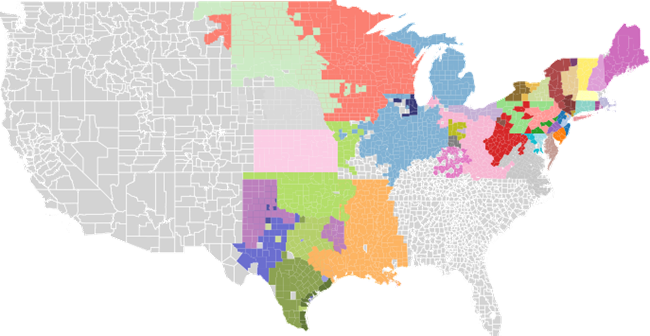
\includegraphics[width=0.5\linewidth]{images/ZoneMap (3).png}
    \caption{Mapped Zones from Market.}
    \label{fig:ZoneMap}
\end{figure}


\begin{figure}[H]
    \centering
    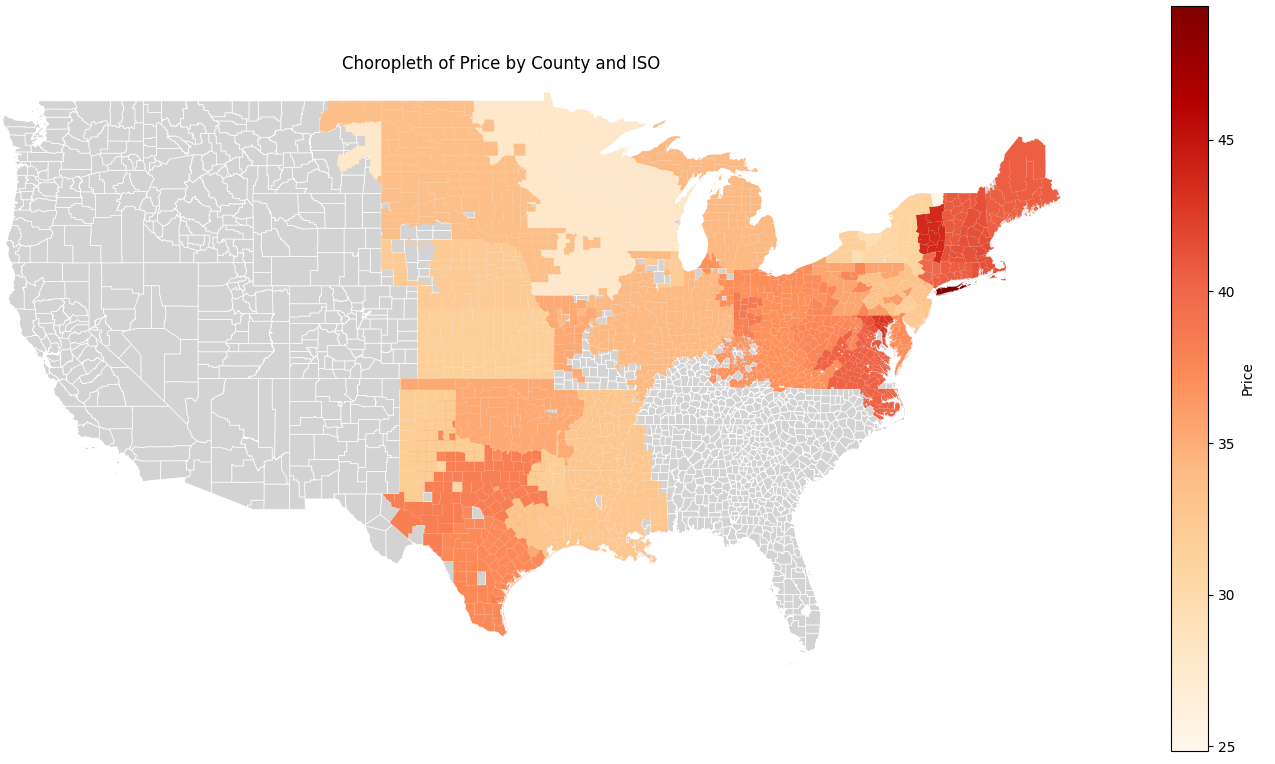
\includegraphics[width=0.5\linewidth]{images/PriceMap (2).png}
    \caption{Locational Marginal Price by Zone in Data.}
    \label{fig:PriceMap}
\end{figure}

\begin{figure}[H]
    \centering
    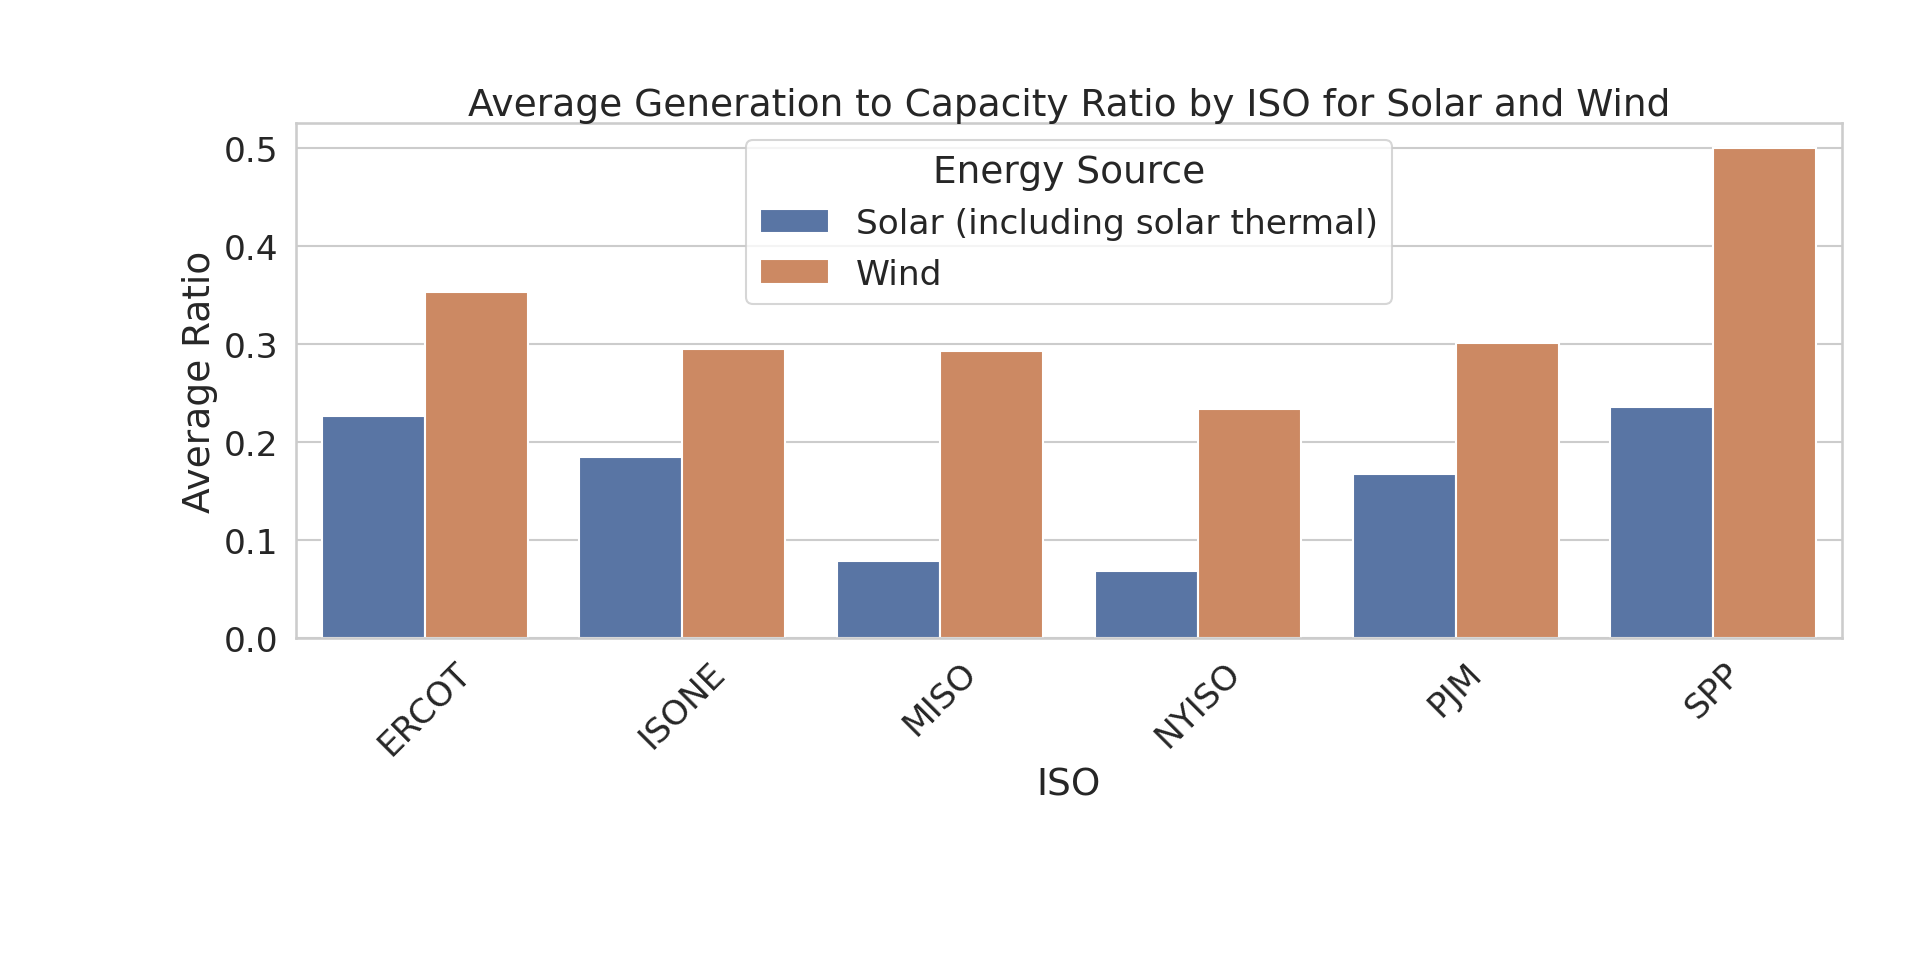
\includegraphics[width=0.5\linewidth]{images/GenerationCapacitySolarWind (1).png}
    \caption{Estimated Capacity Factor for Solar and Wind by ISO.}
    \label{fig:CapacityFactorbyISO}
\end{figure}

\begin{figure}[H]
    \centering
    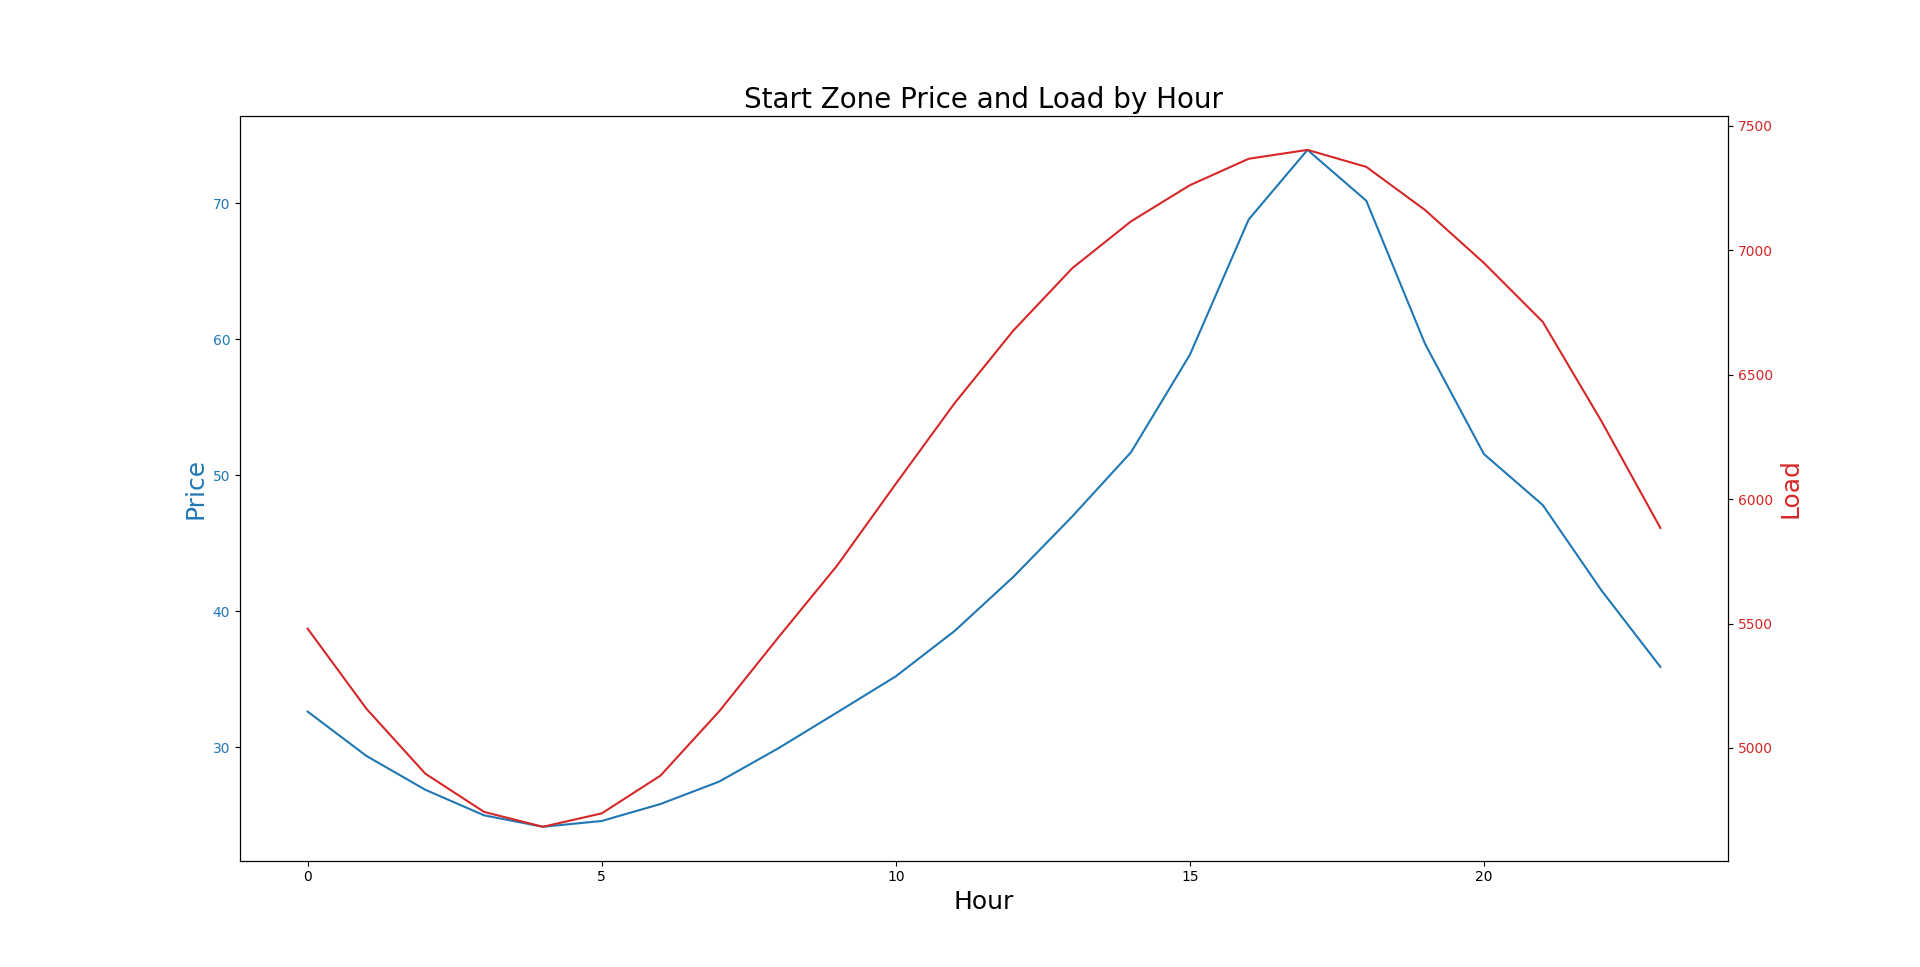
\includegraphics[width=0.5\linewidth]{images/PriceLoadbyHour.png}
    \caption{Price and Load by Hour for entire dataset.}
    \label{fig:PriceLoad}
\end{figure}

\begin{figure}[H]
    \centering
    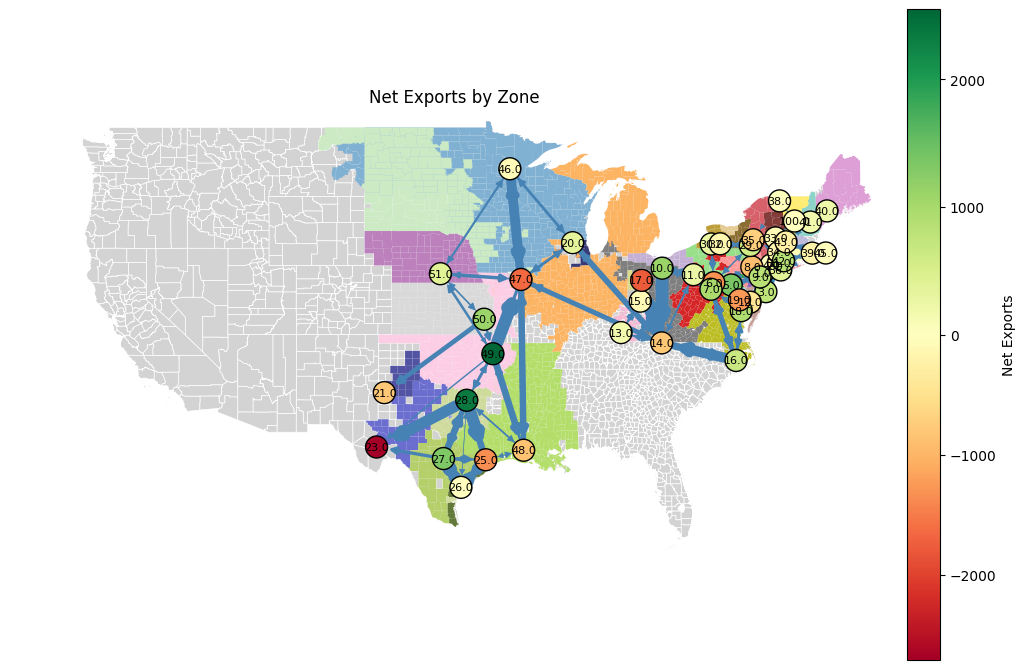
\includegraphics[width=0.5\linewidth]{images/ExportGraph (1).png}
    \caption{Map of Exports between Zones in the Model.}
    \label{ExportGraph}
\end{figure}

% New figures from presentation

\begin{figure}[H]
    \centering
    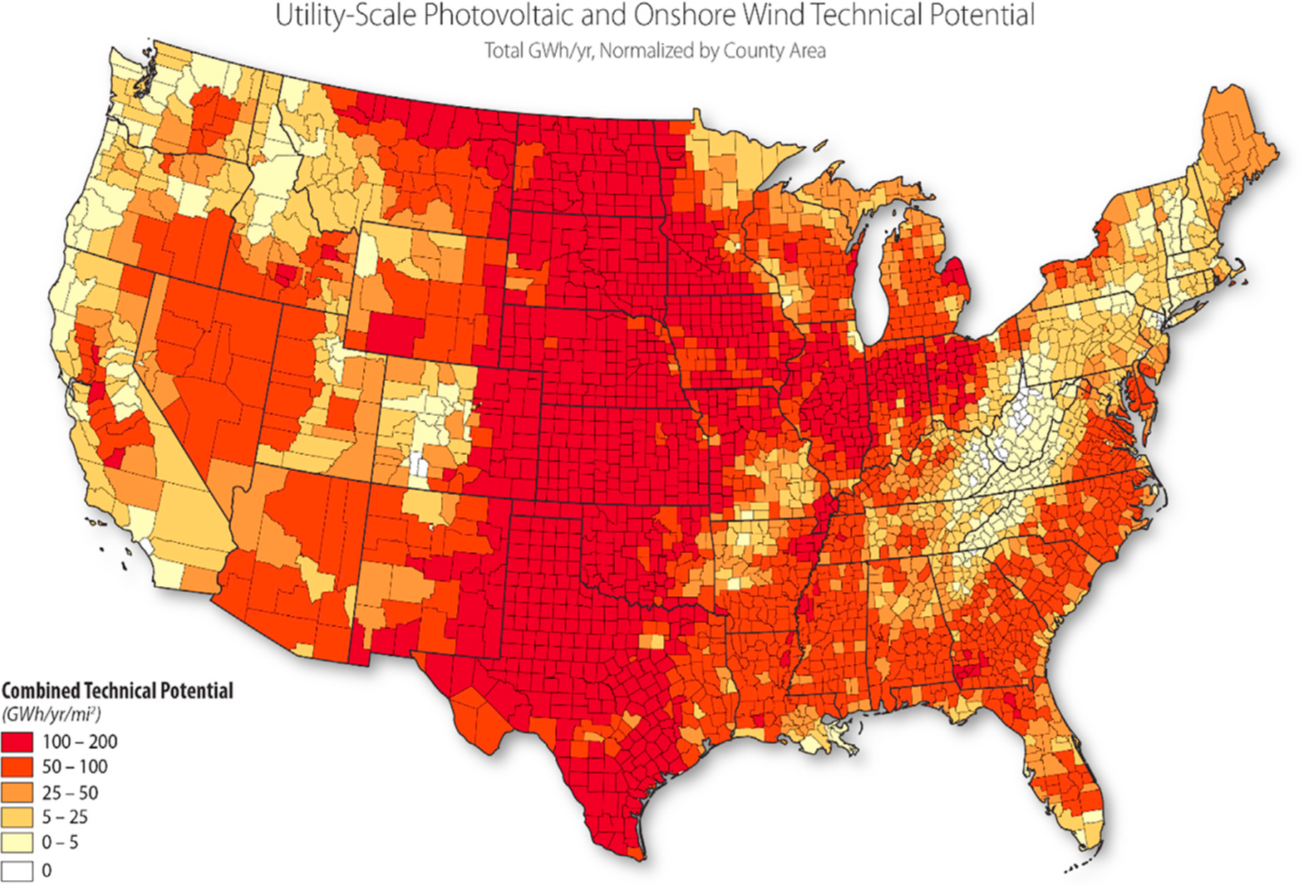
\includegraphics[width=0.8\linewidth]{images/Energy Potential by county.png}
    \caption{Combined Technical Potential for Wind and Solar Generation by County (GWh/yr/mi$^2$). Darker shading indicates higher combined renewable potential. Source: Department of Energy.}
    \label{fig:renewablePotential}
\end{figure}

\begin{figure}[H]
    \centering
    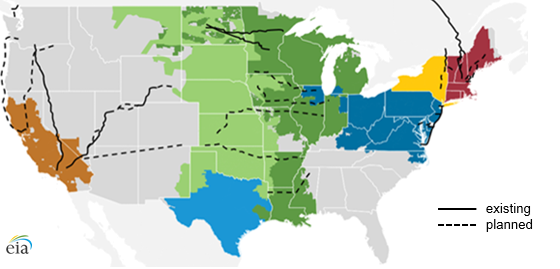
\includegraphics[width=0.8\linewidth]{images/HVDC US.png}
    \caption{Existing and Planned High-Voltage Direct Current Transmission Lines. Solid lines indicate existing HVDC infrastructure; dashed lines indicate proposed expansions. Source: EIA.}
    \label{fig:hvdcLines}
\end{figure}

\begin{figure}[H]
\centering
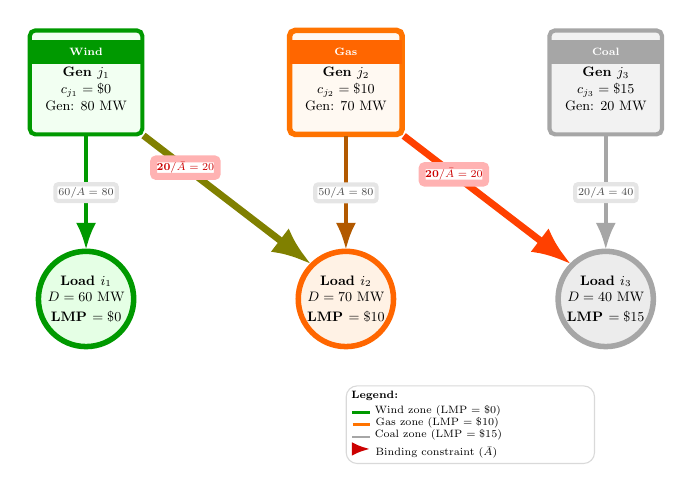
\begin{tikzpicture}[
    scale=0.55, 
    transform shape,
    gen_node/.style={
        rectangle, 
        draw=black!60, 
        thick, 
        rounded corners=2pt, 
        minimum width=2.6cm, 
        minimum height=2.4cm, 
        align=center, 
        fill=white,
        font=\small
    },
    demand_node/.style={
        circle, 
        draw=blue!70!black, 
        thick, 
        minimum size=2.2cm, 
        fill=blue!5,
        align=center,
        font=\small,
        inner sep=1pt
    },
    fuel_header/.style={
        rectangle, 
        minimum width=2.6cm, 
        minimum height=0.55cm, 
        text=white, 
        font=\bfseries\scriptsize, 
        align=center
    },
    edge_label/.style={
        font=\scriptsize, 
        fill=white, 
        text=black!70,
        rounded corners=1pt,
        draw=black!10,
        inner sep=2pt,
        align=center
    },
    infra_marginal/.style={
        gen_node,
        draw=green!60!black,
        line width=1.5pt,
        fill=green!5
    },
    marginal_gen/.style={
        gen_node,
        draw=orange!90!red,
        line width=2pt,
        fill=orange!5
    },
    extra_marginal/.style={
        gen_node,
        draw=gray!70,
        line width=1.5pt,
        fill=gray!10
    },
    transmission/.style={
        -Latex, 
        thick, 
        draw=blue!50!black
    },
    binding_edge/.style={
        -Latex, 
        line width=2.5pt, 
        draw=red!80!black
    },
    binding_label/.style={
        edge_label,
        text=red!80!black,
        font=\bfseries\scriptsize,
        draw=red!30
    },
    lmp_zero/.style={
        demand_node,
        draw=green!60!black,
        line width=2pt,
        fill=green!10
    },
    lmp_mid/.style={
        demand_node,
        draw=orange!80!red,
        line width=2pt,
        fill=orange!10
    },
    lmp_high/.style={
        demand_node,
        draw=gray!70,
        line width=2pt,
        fill=gray!15
    }
]
    % Supply Layer
    \node[infra_marginal] (j1) at (0, 5) {};
    \node[fuel_header, fill=green!60!black] at ([yshift=0.7cm]j1.center) {Wind};
    \node[align=center, font=\small] at ([yshift=-0.15cm]j1.center) {
        \textbf{Gen $j_1$}\\
        $c_{j_1} = \$0$\\
        Gen: 80 MW
    };

    \node[marginal_gen] (j2) at (6, 5) {};
    \node[fuel_header, fill=orange!80!red] at ([yshift=0.7cm]j2.center) {Gas};
    \node[align=center, font=\small] at ([yshift=-0.15cm]j2.center) {
        \textbf{Gen $j_2$}\\
        $c_{j_2} = \$10$\\
        Gen: 70 MW
    };

    \node[extra_marginal] (j3) at (12, 5) {};
    \node[fuel_header, fill=gray!70] at ([yshift=0.7cm]j3.center) {Coal};
    \node[align=center, font=\small] at ([yshift=-0.15cm]j3.center) {
        \textbf{Gen $j_3$}\\
        $c_{j_3} = \$15$\\
        Gen: 20 MW
    };

    % Demand Layer
    \node[lmp_zero] (i1) at (0, 0) {
        \textbf{Load $i_1$}\\
        $D=60$ MW\\[2pt]
        \textbf{LMP $= \$0$}
    };

    \node[lmp_mid] (i2) at (6, 0) {
        \textbf{Load $i_2$}\\
        $D=70$ MW\\[2pt]
        \textbf{LMP $= \$10$}
    };

    \node[lmp_high] (i3) at (12, 0) {
        \textbf{Load $i_3$}\\
        $D=40$ MW\\[2pt]
        \textbf{LMP $= \$15$}
    };

    % Transmission Flows
    \draw[transmission, line width=1.5pt, draw=green!60!black] (j1.south) -- (i1.north) 
        node[midway, edge_label] {$60 / A=80$};
    \draw[binding_edge, draw=green!50!red] (j1.south east) -- (i2.north west) 
        node[pos=0.25, binding_label] {$\mathbf{20} / \bar{A}=20$};
    \draw[transmission, line width=1.5pt, draw=orange!70!black] (j2.south) -- (i2.north) 
        node[midway, edge_label] {$50 / A=80$};
    \draw[binding_edge, draw=orange!50!red] (j2.south east) -- (i3.north west) 
        node[pos=0.3, binding_label] {$\mathbf{20} / \bar{A}=20$};
    \draw[transmission, line width=1.5pt, draw=gray!70] (j3.south) -- (i3.north) 
        node[midway, edge_label] {$20 / A=40$};

    % Legend
    \node[anchor=north west, align=left, font=\scriptsize, 
          draw=gray!30, rounded corners, fill=white,
          text width=5.5cm] at (6.0, -2.0) {
        \textbf{Legend:}\\[2pt]
        \tikz\draw[green!60!black, line width=1.5pt] (0,0) -- (0.4,0); Wind zone (LMP $= \$0$)\\
        \tikz\draw[orange!90!red, line width=2pt] (0,0) -- (0.4,0); Gas zone (LMP $= \$10$)\\
        \tikz\draw[gray!70, line width=1.5pt] (0,0) -- (0.4,0); Coal zone (LMP $= \$15$)\\
        \tikz\draw[red!80!black, line width=2pt, -Latex] (0,0) -- (0.4,0); Binding constraint ($\bar{A}$)
    };
\end{tikzpicture}
\caption{Network Topology Illustrating Congestion Pricing. Binding export constraints create price separation across zones. Each zone's LMP equals the local marginal cost when transmission constraints bind.}
\label{fig:NetworkTopology}
\end{figure}

\begin{figure}[H]
\centering
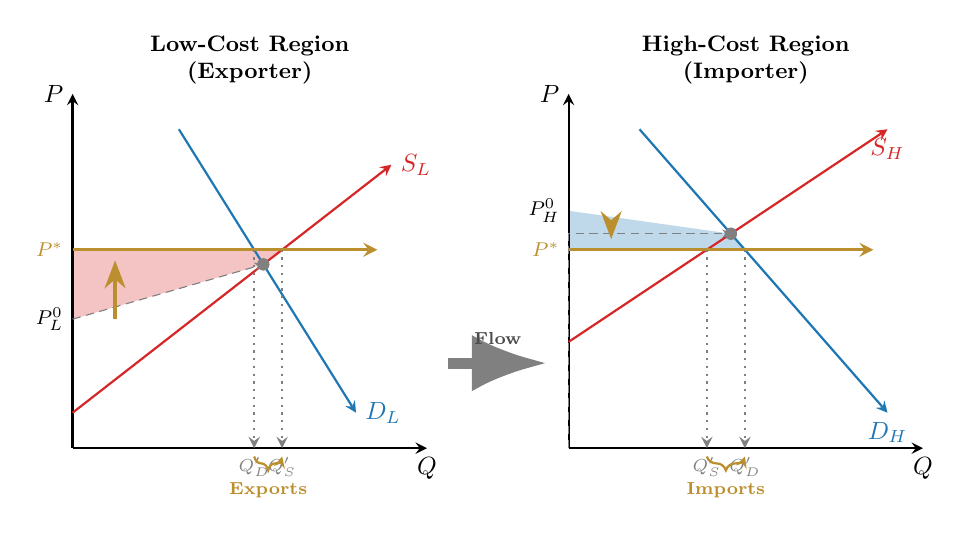
\begin{tikzpicture}[econAxis, scale=0.9, transform shape]

    % LEFT PANEL: EXPORTER
    \begin{scope}[local bounding box=LeftPanel]
        \node[above, font=\small\bfseries, align=center] at (2.5, 5.0) {Low-Cost Region\\(Exporter)};
        
        \draw[econAxis] (0,0) -- (5,0) node[below] {$Q$};
        \draw[econAxis] (0,0) -- (0,5) node[left] {$P$};
        
        \draw[supply, name path=S_L] (0,0.5) -- (4.5,4) node[right] {$S_L$};
        \draw[demand, name path=D_L] (1.5,4.5) -- (4,0.5) node[right] {$D_L$};
        
        \path [name intersections={of=S_L and D_L, by=E_L}];
        \draw[priceLine, name path=priceLine_L_old] (0, 1.82) -- (E_L);
        \node[left, font=\footnotesize] at (0, 1.82) {$P_L^0$};
        \fill[gray] (E_L) circle (2.5pt);

        \coordinate (P_trade_L_start) at (0, 2.8);
        \coordinate (P_trade_L_end) at (4.3, 2.8);
        \draw[very thick, color=econGold, name path=Price_L] (P_trade_L_start) -- (P_trade_L_end);
        \node[left, font=\footnotesize, econGold] at (0, 2.8) {$P^*$};
        
        \path [name intersections={of=S_L and Price_L, by=Q_S_new}];
        \path [name intersections={of=D_L and Price_L, by=Q_D_new}];
        
        \begin{scope}[on background layer]
            \fill[econRed!40, opacity=0.7] (0, 1.82) -- (E_L) -- (Q_S_new) -- (0, 2.8) -- cycle;
        \end{scope}
        
        \draw[dotted, gray] (Q_D_new) -- (Q_D_new |- 0,0) node[below, font=\scriptsize] {$Q_D'$};
        \draw[dotted, gray] (Q_S_new) -- (Q_S_new |- 0,0) node[below, font=\scriptsize] {$Q_S'$};
        
        \draw[decorate, decoration={brace, amplitude=5pt, mirror, raise=3pt}, thick, econGold] 
            (Q_D_new |- 0,0) -- (Q_S_new |- 0,0) 
            node[midway, below=10pt, font=\scriptsize, econGold] {\textbf{Exports}};
        
        \draw[-{Stealth[scale=1.2]}, very thick, econGold] (0.6, 1.82) -- (0.6, 2.65);
    \end{scope}

    % RIGHT PANEL: IMPORTER
    \begin{scope}[shift={(7,0)}, local bounding box=RightPanel]
        \node[above, font=\small\bfseries, align=center] at (2.5, 5.0) {High-Cost Region\\(Importer)};
        
        \draw[econAxis] (0,0) -- (5,0) node[below] {$Q$};
        \draw[econAxis] (0,0) -- (0,5) node[left] {$P$};
        
        \draw[supply, name path=S_H] (0,1.5) -- (4.5,4.5) node[below] {$S_H$};
        \draw[demand, name path=D_H] (1,4.5) -- (4.5,0.5) node[below] {$D_H$};
        
        \path [name intersections={of=S_H and D_H, by=E_H}];
        \draw[priceLine] (0,0) |- (E_H);
        \node[left, font=\footnotesize] at (0, 3.35) {$P_H^0$};
        \fill[gray] (E_H) circle (2.5pt);

        \coordinate (P_trade_H_start) at (0, 2.8);
        \coordinate (P_trade_H_end) at (4.3, 2.8);
        \draw[very thick, color=econGold, name path=Price_H] (P_trade_H_start) -- (P_trade_H_end);
        \node[left, font=\footnotesize, econGold] at (0, 2.8) {$P^*$};
        
        \path [name intersections={of=S_H and Price_H, by=Q_S_H_new}];
        \path [name intersections={of=D_H and Price_H, by=Q_D_H_new}];
        
        \begin{scope}[on background layer]
             \fill[econBlue!40, opacity=0.7] (0, 2.8) -- (Q_D_H_new) -- (E_H) -- (0, 3.35) -- cycle;
        \end{scope}

        \draw[dotted, gray] (Q_S_H_new) -- (Q_S_H_new |- 0,0) node[below, font=\scriptsize] {$Q_S'$};
        \draw[dotted, gray] (Q_D_H_new) -- (Q_D_H_new |- 0,0) node[below, font=\scriptsize] {$Q_D'$};

        \draw[decorate, decoration={brace, amplitude=5pt, mirror, raise=3pt}, thick, econGold] 
            (Q_S_H_new |- 0,0) -- (Q_D_H_new |- 0,0) 
            node[midway, below=10pt, font=\scriptsize, econGold] {\textbf{Imports}};

        \draw[-{Stealth[scale=1.2]}, very thick, econGold] (0.6, 3.2) -- (0.6, 2.95);
    \end{scope}

    % CONNECTOR
    \draw[line width=4pt, -{Latex[scale=1.3]}, color=black!50] (5.3, 1.2) -- (6.7, 1.2);
    \node[font=\scriptsize\bfseries, color=black!70] at (6, 1.55) {Flow};

\end{tikzpicture}
\caption{Static Effects of Transmission Expansion: Price Convergence and Spatial Arbitrage. In the low-cost (exporting) region, prices rise and producer surplus increases (red shaded area). In the high-cost (importing) region, prices fall and consumer surplus increases (blue shaded area).}
\label{fig:StaticEffects}
\end{figure}

\begin{figure}[H]
\centering
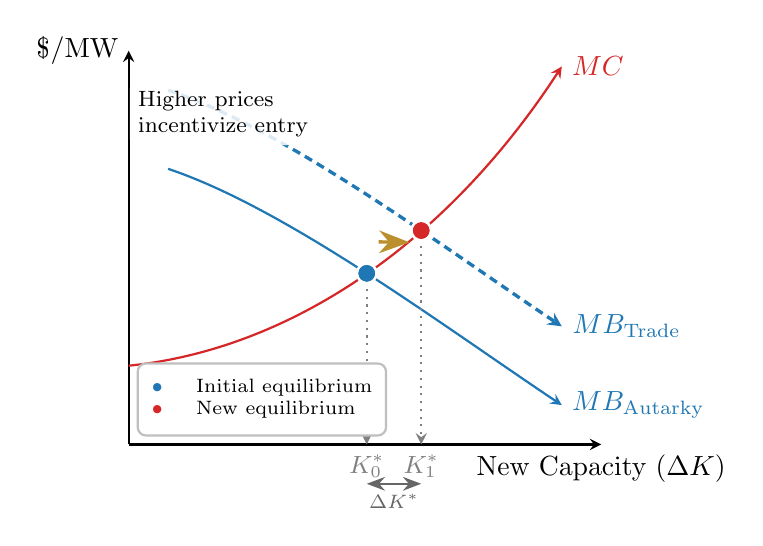
\begin{tikzpicture}[scale=1.0, econAxis, transform shape]
    
    % Axes
    \draw[econAxis] (0,0) -- (6,0) node[below] {New Capacity ($\Delta K$)};
    \draw[econAxis] (0,0) -- (0,5) node[left] {\$/MW};

    % Marginal Cost
    \draw[supply, name path=MC] (0,1) .. controls (2,1.2) and (4,2.5) .. (5.5,4.8) 
        node[right] {$MC$};

    % MB Original
    \draw[demand, name path=MB0] (0.5,3.5) .. controls (2,3) and (4,1.5) .. (5.5,0.5) 
        node[right] {$MB_{\text{Autarky}}$};

    % MB New
    \draw[demand, densely dashed, line width=1.2pt, name path=MB1] 
        (0.5,4.5) .. controls (2,4) and (4,2.5) .. (5.5,1.5) 
        node[right] {$MB_{\text{Trade}}$};

    % Equilibria
    \path [name intersections={of=MC and MB0, by=E0}];
    \path [name intersections={of=MC and MB1, by=E1}];

    % Drop lines
    \draw[dotted, gray, thick] (E0) -- (E0 |- 0,0) node[below, font=\small] {$K^*_0$};
    \draw[dotted, gray, thick] (E1) -- (E1 |- 0,0) node[below, font=\small] {$K^*_1$};
    
    % Points
    \fill[econBlue] (E0) circle (3.5pt);
    \fill[econRed] (E1) circle (3.5pt);
    \draw[white, line width=1pt] (E0) circle (3.5pt);
    \draw[white, line width=1pt] (E1) circle (3.5pt);
    \fill[econBlue] (E0) circle (3pt);
    \fill[econRed] (E1) circle (3pt);

    % Annotation
    \draw[-{Stealth[scale=1.3]}, very thick, econGold] 
        ($(E0)+(0.15,0.4)$) -- ($(E1)+(-0.15, -0.15)$);
    
    \node[font=\footnotesize, align=left, fill=white, fill opacity=0.85, 
          text opacity=1, inner sep=3pt, rounded corners=2pt] 
        at (1.2, 4.2) 
        {Higher prices\\incentivize entry};

    % Legend
    \node[draw=gray!50, rounded corners=3pt, inner sep=5pt, font=\scriptsize,
          fill=white, anchor=south west] at (0.1, 0.1) {
        \begin{tabular}{@{}cl@{}}
            \textcolor{econBlue}{$\bullet$} & Initial equilibrium \\
            \textcolor{econRed}{$\bullet$} & New equilibrium
        \end{tabular}
    };

    % Capacity expansion
    \draw[{Stealth}-{Stealth}, thick, black!60] 
        ($(E0 |- 0,0) + (0, -0.5)$) -- ($(E1 |- 0,0) + (0, -0.5)$)
        node[midway, below, font=\scriptsize] {$\Delta K^*$};

\end{tikzpicture}
\caption{Dynamic Effects of Transmission Expansion: The Investment Signal. Expanded market access shifts the marginal benefit curve outward for generators in resource-rich regions, leading to increased equilibrium capacity investment.}
\label{fig:DynamicEffects}
\end{figure}

\begin{figure}[H]
\centering
% The resizebox only wraps the tikzpicture
\resizebox{0.98\textwidth}{!}{%
    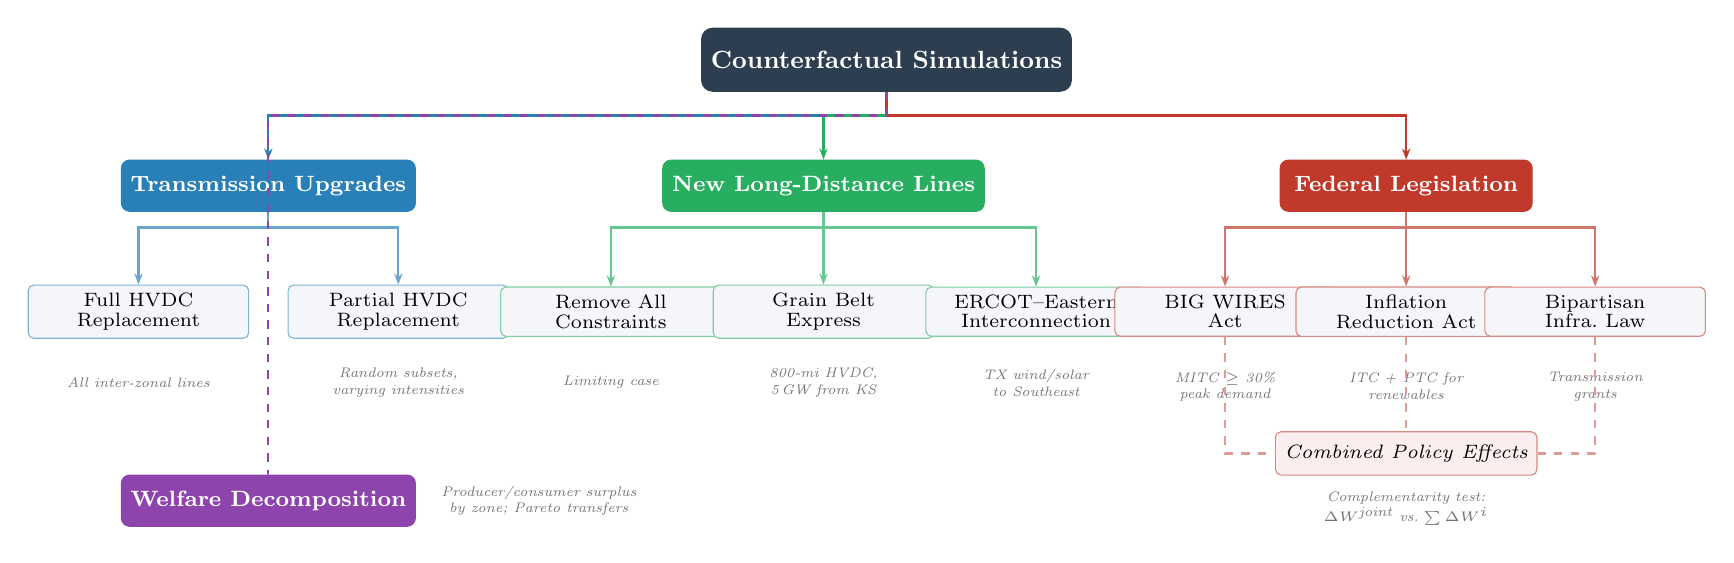
\begin{tikzpicture}[
        root/.style={
            rectangle, rounded corners=4pt, draw=rootcolor, fill=rootcolor,
            text=white, font=\bfseries\small, minimum height=0.8cm,
            minimum width=3.6cm, align=center
        },
        category/.style={
            rectangle, rounded corners=3pt, draw=#1, fill=#1,
            text=white, font=\bfseries\footnotesize, minimum height=0.65cm,
            minimum width=3.2cm, align=center
        },
        leaf/.style={
            rectangle, rounded corners=2pt, draw=#1!60, fill=leafbg,
            text=black, font=\scriptsize, minimum height=0.55cm,
            minimum width=2.8cm, align=center, inner sep=3pt
        },
        combined/.style={
            rectangle, rounded corners=2pt, draw=catC!60, fill=catC!8,
            text=black, font=\scriptsize\itshape, minimum height=0.55cm,
            minimum width=2.8cm, align=center
        },
        arrow/.style={-{Stealth[length=4pt]}, thick, color=#1},
        note/.style={font=\tiny\itshape, text=black!55, align=center},
    ]

    % Root
    \node[root] (root) at (0,0) {Counterfactual Simulations};

    % ---- Category nodes ----
    \node[category=catA] (catTU) at (-7.85, -1.6) {Transmission Upgrades};
    \node[category=catB] (catNT) at (-0.8, -1.6) {New Long-Distance Lines};
    \node[category=catC] (catFL) at (6.6, -1.6) {Federal Legislation};

    % ---- Transmission Upgrades leaves ----
    \node[leaf=catA] (tu1) at (-9.5, -3.2) {Full HVDC\\[-1pt]Replacement};
    \node[leaf=catA] (tu2) at (-6.2, -3.2) {Partial HVDC\\[-1pt]Replacement};

    % ---- New Transmission leaves ----
    \node[leaf=catB] (nt1) at (-3.5, -3.2) {Remove All\\[-1pt]Constraints};
    \node[leaf=catB] (nt2) at (-0.8, -3.2) {Grain Belt\\[-1pt]Express};
    \node[leaf=catB] (nt3) at (1.9, -3.2) {ERCOT--Eastern\\[-1pt]Interconnection};

    % ---- Federal Legislation leaves ----
    \node[leaf=catC] (fl1) at (4.3, -3.2) {BIG WIRES\\[-1pt]Act};
    \node[leaf=catC] (fl2) at (6.6, -3.2) {Inflation\\[-1pt]Reduction Act};
    \node[leaf=catC] (fl3) at (9.0, -3.2) {Bipartisan\\[-1pt]Infra.\ Law};

    % Combined policy
    \node[combined] (fl4) at (6.6, -5.0) {Combined Policy Effects};

    % ---- Annotations ----
    \node[note] at (-9.5, -4.1) {All inter-zonal lines};
    \node[note] at (-6.2, -4.1) {Random subsets,\\varying intensities};
    \node[note] at (-3.5, -4.1) {Limiting case};
    \node[note] at (-0.8, -4.1) {800-mi HVDC,\\5\,GW from KS};
    \node[note] at (1.9, -4.1) {TX wind/solar\\to Southeast};
    \node[note] at (4.3, -4.15) {MITC $\geq$ 30\%\\peak demand};
    \node[note] at (6.6, -4.15) {ITC + PTC for\\renewables};
    \node[note] at (9.0, -4.15) {Transmission\\grants};
    \node[note] at (6.6, -5.7) {Complementarity test:\\$\Delta W^{\text{joint}}$ vs.\ $\sum \Delta W^{i}$};

    % ---- Welfare Decomposition ----
    \node[category=catD] (wd) at (-7.85, -5.6) {Welfare Decomposition};
    \node[note, right=0.2cm of wd] {Producer/consumer surplus\\by zone; Pareto transfers};

    % ---- Edges: root to categories ----
    \draw[arrow=catA] (root.south) -- ++(0,-0.3) -| (catTU.north);
    \draw[arrow=catB] (root.south) -- ++(0,-0.3) -| (catNT.north);
    \draw[arrow=catC] (root.south) -- ++(0,-0.3) -| (catFL.north);

    % ---- Edges: categories to leaves ----
    \draw[arrow=catA!70] (catTU.south) -- ++(0,-0.2) -| (tu1.north);
    \draw[arrow=catA!70] (catTU.south) -- ++(0,-0.2) -| (tu2.north);

    \draw[arrow=catB!70] (catNT.south) -- ++(0,-0.2) -| (nt1.north);
    \draw[arrow=catB!70] (catNT.south) -- ++(0,-0.2) -| (nt2.north);
    \draw[arrow=catB!70] (catNT.south) -- ++(0,-0.2) -| (nt3.north);

    \draw[arrow=catC!70] (catFL.south) -- ++(0,-0.2) -| (fl1.north);
    \draw[arrow=catC!70] (catFL.south) -- ++(0,-0.2) -| (fl2.north);
    \draw[arrow=catC!70] (catFL.south) -- ++(0,-0.2) -| (fl3.north);

    % Dashed to combined
    \draw[dashed, catC!50, thick] (fl1.south) |- (fl4.west);
    \draw[dashed, catC!50, thick] (fl2.south) -- (fl4.north);
    \draw[dashed, catC!50, thick] (fl3.south) |- (fl4.east);

    % Welfare decomposition arrow (dashed from root)
    \draw[arrow=catD, dashed] (root.south) -- ++(0,-0.3) -- ++(-7.85, 0) |- (wd.north);

    \end{tikzpicture}%
} % End of resizebox

\caption{Visual description of counterfactuals run and how they relate.}
\label{fig:CounterfactualSimulations}

\end{figure}


%\begin{figure}[hp]
%  \centering
%  \includegraphics[width=.6\textwidth]{../fig/placeholder.pdf}
%  \caption{Placeholder}
%  \label{fig:placeholder}
%\end{figure}




\clearpage

\appendix

\section{Solving the Operations Model}\label{app:operations}

This appendix derives the likelihood function used to estimate the short-run operations model. Section~\ref{app:iso_problem} establishes the equivalence between the generator profit maximization problem and a social planner's cost minimization problem, then formulates the ISO's dispatch problem. Section~\ref{app:focs} derives the first-order conditions from the Lagrangian. Section~\ref{app:likelihood} specifies the cost function and derives the likelihood function for estimation.

\subsection{The ISO Dispatch Problem}\label{app:iso_problem}

Under standard conditions, the generator's profit maximization problem is equivalent to a social planner's cost minimization problem. Following \cite{gilbert2004allocating} and \cite{cramton2017electricity}, the conditions for this equivalence include: (i) no market power among generators, (ii) no gamesmanship or non-competitive bidding, (iii) increasing marginal cost curves, and (iv) linear constraints. The assumption of increasing marginal costs is consistent with both bid offer data and economic theory. Gamesmanship and non-competitive bidding are prohibited and actively monitored by the Federal Energy Regulatory Commission. While transmission constraints can create local market power (\cite{gilbert2004allocating}), competitive pressures and regulatory limits on bidding behavior make sustained market power difficult to maintain.

I aggregate to the resource and ISO level due to data limitations: hourly generation data are available only at the resource level rather than the generator level. While this aggregation sacrifices granularity that would be valuable in a transmission model, I disaggregate where data permit.

\subsubsection{Notation}

Let $i \in \{1, \ldots, I\}$ index demand nodes, $j \in \{1, \ldots, J\}$ index supply (generation) nodes, $k \in \{1, \ldots, K\}$ index resources at each supply node, and $t \in \{1, \ldots, T\}$ index time periods (hours). Define:
\begin{itemize}
    \item $q_{ijkt}$: Quantity of electricity sent from resource $k$ at supply node $j$ to demand node $i$ at time $t$
    \item $c_{jkt}(\cdot)$: Cost function for resource $k$ at supply node $j$ at time $t$
    \item $x_{jkt}$: Observable cost shifters for resource $jk$ at time $t$
    \item $\epsilon_{ijkt}$: Unobserved cost shock
    \item $A_{ij}$: Transmission capacity between nodes $i$ and $j$
    \item $O_{jkt}^{MAX}$: Maximum generation capacity of resource $k$ at node $j$ at time $t$
    \item $L_{it}$: Load (demand) at node $i$ at time $t$
    \item $B_{ij}$: Transmission loss factor between nodes $i$ and $j$
\end{itemize}

\subsubsection{The Optimization Problem}

The ISO solves a static cost minimization problem each hour, choosing dispatch quantities $q_{ijkt}$ to minimize the total cost of meeting demand:
\begin{equation}\label{eq:objective}
    \pi_{t} = \max_{\{q_{ijkt}\}} \left[ -\sum_{j=1}^{J} \sum_{k=1}^{K} c_{jkt}\left(x_{jkt}, \sum_{i=1}^{I} q_{ijkt}, \sum_{i=1}^{I} \epsilon_{ijkt}\right) \right]
\end{equation}
subject to three constraints.

\paragraph{Transmission Constraint.} Flows between any two nodes cannot exceed line capacity:
\begin{equation}\label{eq:transmission}
    \sum_{k=1}^{K} q_{ijkt} \leq A_{ij} \quad \forall \, i, j, t.
\end{equation}

\paragraph{Capacity Constraint.} Total dispatch from each resource cannot exceed its maximum capacity:
\begin{equation}\label{eq:capacity}
    0 \leq \sum_{i=1}^{I} q_{ijkt} \leq O_{jkt}^{MAX} \quad \forall \, j, k, t.
\end{equation}

\paragraph{Load Balance Constraint.} Supply must equal demand at each node, accounting for transmission losses:
\begin{equation}\label{eq:load_balance}
    \sum_{j=1}^{J} \sum_{k=1}^{K} (1 - B_{ij}) q_{ijkt} = L_{it} \quad \forall \, i, t.
\end{equation}

Three maintained assumptions ensure the problem is well-defined: (i) no blackouts, meaning sufficient generation capacity exists to serve all load at every node; (ii) no resource is transmission-constrained to all destinations; and (iii) at least one resource at each generation node has slack capacity at any given time.

When no constraints bind, resources set marginal cost equal to price and serve the highest-priced locations first. When the transmission constraint binds, a resource dispatches up to $A_{ij} - \sum_{k' \neq k} q_{ijk't}$ units to the highest-priced location, then up to $A_{ij}$ units to the next highest-priced location, continuing until either maximum capacity $O_{jkt}^{MAX}$ is reached or marginal revenue equals marginal cost. Prices equal the marginal cost of the last economically dispatched resource at each location.

\subsection{First-Order Conditions}\label{app:focs}

The Lagrangian for the ISO's problem at time $t$ is:
\begin{align}\label{eq:lagrangian}
    \mathcal{L}_t = & -\sum_{k=1}^{K} \sum_{j=1}^{J} c_{jkt}\left(x_{jkt}, \sum_{i=1}^{I} q_{ijkt}, \sum_{i=1}^{I} \epsilon_{ijkt}\right) \nonumber \\
    & + \sum_{i,j} \lambda_{ijt} \left(A_{ij} - \sum_{k=1}^{K} q_{ijkt}\right) \nonumber \\
    & + \sum_{i} \gamma_{it} \left(L_{it} - \sum_{k=1}^{K} \sum_{j=1}^{J} (1 - B_{ij}) q_{ijkt}\right) \nonumber \\
    & + \sum_{j,k} \theta_{jkt} \left(O_{jkt}^{MAX} - \sum_{i=1}^{I} q_{ijkt}\right),
\end{align}
where $\lambda_{ijt}$ is the multiplier on the transmission constraint, $\gamma_{it}$ is the multiplier on the load balance constraint, and $\theta_{jkt}$ is the multiplier on the capacity constraint.

\subsubsection{Optimality Conditions}

The first-order condition with respect to $q_{ijkt}$ is:
\begin{equation}\label{eq:foc}
    \frac{\partial \mathcal{L}_t}{\partial q_{ijkt}} = -\frac{\partial c_{jkt}}{\partial q_{ijkt}} - \lambda_{ijt} - \gamma_{it}(1 - B_{ij}) - \theta_{jkt} = 0.
\end{equation}

Complementary slackness requires:
\begin{align}
    \lambda_{ijt} \left(A_{ij} - \sum_{k=1}^{K} q_{ijkt}\right) &= 0 \quad \forall \, i, j, t, \label{eq:cs_trans} \\
    \theta_{jkt} \left(O_{jkt}^{MAX} - \sum_{i=1}^{I} q_{ijkt}\right) &= 0 \quad \forall \, j, k, t. \label{eq:cs_cap}
\end{align}

Rearranging equation~\eqref{eq:foc} yields three equivalent expressions:
\begin{align}
    \frac{\partial c_{jkt}}{\partial q_{ijkt}} + \gamma_{it}(1 - B_{ij}) + \theta_{jkt} &= \lambda_{ijt}, \label{eq:foc_lambda} \\
    \frac{\partial c_{jkt}}{\partial q_{ijkt}} + \gamma_{it}(1 - B_{ij}) + \lambda_{ijt} &= \theta_{jkt}, \label{eq:foc_theta} \\
    \frac{\partial c_{jkt}}{\partial q_{ijkt}} + \lambda_{ijt} + \theta_{jkt} &= \gamma_{it}(1 - B_{ij}). \label{eq:foc_gamma}
\end{align}

\subsubsection{Intratemporal Euler Conditions}

Three key relationships emerge from comparing first-order conditions across different resource-node combinations.

\paragraph{Condition 1: Same supply node, different resources.} For two resources $k$ and $k'$ at the same supply node $j$, both sending to demand node $i$:
\begin{equation}\label{eq:euler1}
    \frac{\partial c_{jkt}}{\partial q_{ijkt}} + \theta_{jkt} = \frac{\partial c_{jk't}}{\partial q_{ijk't}} + \theta_{jk't}.
\end{equation}

\paragraph{Condition 2: Same resource, different demand nodes.} For resource $k$ at supply node $j$ sending to two demand nodes $i$ and $i'$:
\begin{equation}\label{eq:euler2}
    \frac{\partial c_{jkt}}{\partial q_{ijkt}} + \gamma_{it}(1 - B_{ij}) + \lambda_{ijt} = \frac{\partial c_{jkt}}{\partial q_{i'jkt}} + \gamma_{i't}(1 - B_{i'j}) + \lambda_{i'jt}.
\end{equation}

\paragraph{Condition 3: Different supply nodes, same demand node.} For resources at different supply nodes $jk$ and $j'k'$ both sending to demand node $i$:
\begin{equation}\label{eq:euler3}
    \frac{\partial c_{jkt}}{\partial q_{ijkt}} + \lambda_{ijt} + \theta_{jkt} = \frac{(1 - B_{ij})}{(1 - B_{ij'})} \left[\frac{\partial c_{j'k't}}{\partial q_{ij'k't}} + \lambda_{ij't} + \theta_{j'k't}\right].
\end{equation}

\subsection{Cost Function Specification and Likelihood}\label{app:likelihood}

\subsubsection{Cost Function}

For renewable resources (wind and solar), the cost function is linear in output:
\begin{equation}
    c_{jkt}^{renew} = q_{ijkt} \epsilon_{ijkt}.
\end{equation}

For non-renewable resources, the cost function is quadratic:
\begin{equation}\label{eq:cost_nonrenew}
    c_{jkt} = \sum_{i=1}^{I} q_{ijkt} x_{jkt} \beta + \frac{1}{2} \left(\sum_{i=1}^{I} q_{ijkt}\right)^2 \nu_k + \sum_{i=1}^{I} q_{ijkt} \epsilon_{ijkt},
\end{equation}
where $\beta$ and $\nu_k$ are parameters to be estimated, with $\nu_k$ varying by resource type to capture differences in fuel costs. The marginal cost for non-renewable resources is:
\begin{equation}\label{eq:mc}
    \frac{\partial c_{jkt}}{\partial q_{ijkt}} = x_{jkt} \beta + q_{ijkt} \nu_k + \epsilon_{ijkt}.
\end{equation}

\subsubsection{Identifying the Central Resource}

Define a \emph{central resource} at each demand node as a resource for which neither the transmission constraint nor the capacity constraint binds: $\lambda_{ijt} = 0$ and $\theta_{jkt} = 0$. By the no-blackout assumption, every demand node has at least one central resource. For central resources, the observed locational marginal price (LMP) equals marginal cost:
\begin{equation}
    \frac{\partial c_{jkt}}{\partial q_{ijkt}} = LMP_{it}.
\end{equation}

Using equation~\eqref{eq:euler3} with a central resource $j''k''$ at node $i$:
\begin{equation}\label{eq:central}
    \frac{\partial c_{jkt}}{\partial q_{ijkt}} + \lambda_{ijt} + \theta_{jkt} = \frac{(1 - B_{ij})}{(1 - B_{ij''})} LMP_{it}.
\end{equation}

Rearranging and substituting the marginal cost specification:
\begin{equation}\label{eq:error_eq}
    x_{jkt} \beta + q_{ijkt} \nu_k + \lambda_{ijt} + \theta_{jkt} - \frac{(1 - B_{ij})}{(1 - B_{ij''})} LMP_{it} = -\epsilon_{ijkt}.
\end{equation}

\subsubsection{Solving for Shadow Prices}

From equation~\eqref{eq:foc_gamma} applied to the central resource at node $i$:
\begin{equation}\label{eq:gamma}
    \gamma_{it} = \frac{LMP_{it}}{(1 - B_{ij''})}.
\end{equation}

\paragraph{Transmission Shadow Price.} Using equation~\eqref{eq:euler2} and the assumption that each resource can send electricity to at least one unconstrained destination $i'$ (so $\lambda_{i'jt} = 0$):
\begin{equation}\label{eq:lambda}
    \lambda_{ijt} = q_{i'jkt} \nu_k - q_{ijkt} \nu_k + \frac{LMP_{i't}}{(1 - B_{i'j''})}(1 - B_{i'j}) - \frac{LMP_{it}}{(1 - B_{ij'''})}(1 - B_{ij}) + \epsilon_{i'jkt} - \epsilon_{ijkt},
\end{equation}
where $j''$ and $j'''$ denote the central resources at nodes $i'$ and $i$, respectively.

\paragraph{Capacity Shadow Price.} Using equation~\eqref{eq:euler1} and the assumption that each generation node has at least one resource $k'$ with slack capacity (so $\theta_{jk't} = 0$):
\begin{equation}\label{eq:theta}
    \theta_{jkt} = (x_{jk't} \beta + q_{ijk't} \nu_{k'}) - (x_{jkt} \beta + q_{ijkt} \nu_k) + \epsilon_{ijk't} - \epsilon_{ijkt}.
\end{equation}

\subsubsection{Constructing the Likelihood Function}

Substituting the expressions for $\lambda_{ijt}$ and $\theta_{jkt}$ into equation~\eqref{eq:error_eq} yields the estimating equation. Define the composite error:
\begin{equation}\label{eq:composite_error}
    \tilde{\epsilon}_{ijkt} = \epsilon_{ijkt} - \epsilon_{i'jkt} - \epsilon_{ijk't},
\end{equation}
where $i'$ is the unconstrained destination for resource $jk$ and $k'$ is the unconstrained resource at node $j$.

The deterministic component of the estimating equation is:
\begin{align}\label{eq:V}
    \tilde{V}_{ijkt} = \; & \underbrace{x_{jkt} \beta + q_{ijkt} \nu_k}_{\text{MC of resource } jk} - \underbrace{\frac{(1 - B_{ij})}{(1 - B_{ij''})} LMP_{it}}_{\text{MC of central resource}} \nonumber \\
    & + \underbrace{q_{i'jkt} \nu_k - q_{ijkt} \nu_k + \frac{LMP_{i't}}{(1 - B_{i'j''})}(1 - B_{i'j}) - \frac{LMP_{it}}{(1 - B_{ij'''})}(1 - B_{ij})}_{\text{cost of transmission constraint}} \nonumber \\
    & + \underbrace{(x_{jk't} \beta + q_{ijk't} \nu_{k'}) - (x_{jkt} \beta + q_{ijkt} \nu_k)}_{\text{cost of capacity constraint}}.
\end{align}

For resources with transmission constraints but no capacity constraints:
\begin{equation}
    \tilde{\epsilon}_{ijk't} = \epsilon_{ijk't} - \epsilon_{i'jk't}.
\end{equation}

For resources with neither constraint binding:
\begin{equation}
    \tilde{\epsilon}_{i'jk't} = \epsilon_{i'jk't}.
\end{equation}

By substitution, each individual error $\epsilon_{ijkt}$ can be recovered.

\subsubsection{Maximum Likelihood Estimation}

Let $P_t(\cdot)$ denote a multivariate normal density with mean zero and variance-covariance matrix $\Omega$. The likelihood function is:
\begin{equation}\label{eq:likelihood}
    \mathcal{L} = \prod_{t=1}^{T} P_t\left(\tilde{V}_{111t}, \ldots, \tilde{V}_{IJKt}\right).
\end{equation}

Maximizing this likelihood function yields estimates of $\beta$ (the effect of observable cost shifters) and $\nu_k$ (resource-type-specific marginal cost parameters), thereby recovering the short-run cost structure.

\section{Long-run Model Computational Details} \label{sec:appendixb}
\addcontentsline{toc}{section}{Appendix B: Long-run Model Computational Details}

\subsection{Algorithm Overview}\label{sec:algorithm_overview}

This appendix details the computational methodology for estimating the long-run capacity investment model. The estimation combines a nested fixed point algorithm for computing equilibrium with generalized method of moments (GMM) estimation for parameter recovery. The approach follows the dynamic game estimation methodology developed by \cite{pakes1998empirical} and utilizes algorithmic improvements from \cite{gowrisankaran2024computable} to identify feasible choices and accelerate convergence.

The computational procedure consists of three main components: (i) state space discretization, (ii) equilibrium computation via nested fixed point iteration, and (iii) GMM estimation using simulated moments. Each component is described in detail below.

\subsection{State Space Discretization}\label{sec:state_space}

The dynamic investment problem is solved over a discretized approximation to the continuous state space. Discretization renders the Bellman equation computationally tractable while preserving economically relevant variation in prices, quantities, and profits. The grid is constructed to capture empirically observed ranges of capacity, demand, and prices, with bounds chosen to exceed historical maxima to accommodate counterfactual investment paths.

\subsubsection{State Variable Bins}\label{subsec:state_bins}

The state space is discretized as shown in Table \ref{tab:state_space}. Each state variable is discretized using evenly spaced bins over a bounded interval informed by historical data and engineering constraints.

\begin{table}[htbp]
\centering
\caption{State Space Discretization}
\label{tab:state_space}
\begin{tabular}{lcc}
\toprule
State Variable & Bins & Range \\
\midrule
Fixed cost ($F_k$) & 20 & $[0, \bar{R}_k]$ \\
Entry cost ($E_k$) & 20 & $[0, 10 \times \bar{R}_k]$ \\
Demand state & 5 & $[0.75 \times \bar{L}, 1.5 \times \bar{L}]$ \\
Own capacity ($O_{jkg}$) & 15 & $[0, 1.5 \times \bar{G}_{jg}]$ \\
Rival capacity ($O_{jkg}^-$) & 10 & $[0, 1.5 \times \bar{L}]$ \\
Average price ($P_{jkg}$) & 10 & $[0, 1.1 \times \bar{P}]$ \\
\bottomrule
\end{tabular}
\begin{minipage}{0.9\textwidth}
\vspace{0.5em}
\footnotesize
\textit{Notes:} $\bar{R}_k$ denotes maximum observed revenue per MW for resource type $k$; $\bar{L}$ denotes the historical maximum system load; $\bar{G}_{jg}$ denotes the maximum observed generation by owner $g$ in region $j$; and $\bar{P}$ denotes the historical maximum average price.
\end{minipage}
\end{table}

Demand uncertainty is modeled using a multiplicative demand scaling factor applied to historical load profiles. The five demand states span $\pm 25\%$ around baseline demand and are intended to capture persistent variation in system conditions rather than transitory hourly shocks.

Own capacity and rival capacity are discretized separately. Own capacity reflects firm-specific investment decisions, while rival capacity aggregates the competitive fringe and other strategic firms into a single state variable, consistent with an oblivious equilibrium approximation. Capacity bounds exceed historical maxima to allow for endogenous entry and expansion in counterfactual scenarios.

\subsubsection{Short-Run Outcome Mapping}

For each point in the discretized state space, the model computes short-run equilibrium outcomes by solving a linear or quadratic dispatch problem subject to generator capacity constraints, zonal load balance, and transmission limits (see Section \ref{sec:appendixc}). The solution yields locational marginal prices, dispatched quantities, production costs, and operating profits.

Outcomes are computed as weighted averages across representative operating conditions (e.g., seasonal or load-duration blocks), producing a smooth mapping from state variables to expected period profits. These expected profits are stored and treated as primitives in the dynamic investment problem.

\subsubsection{Investment Choice Set}

The firm’s investment choice is restricted to a discrete set of ten capacity adjustment options. These include incremental additions for expanding technologies and retirement options for declining resources. Capacity is constrained to remain weakly non-negative, ruling out infeasible states. This restriction substantially reduces the dimensionality of the choice set while preserving the economically relevant margins of adjustment.

\subsubsection{Approximation Accuracy and Computational Feasibility}

The number of bins for each state variable reflects a tradeoff between approximation accuracy and computational feasibility. Finer grids are used for own capacity and cost states, which directly affect firm profits, while coarser grids are used for rival capacity and prices. Sensitivity checks using alternative grid densities yield similar qualitative investment patterns, indicating that results are not driven by discretization artifacts.

The full state space is evaluated using batched computation with intermediate checkpointing, enabling parallel execution and recovery from job interruption. This approach allows the model to evaluate tens of thousands of state points per resource type while maintaining feasible memory and runtime requirements. A schematic overview of the dataset construction is provided in Figure \ref{DataSetCreation}.

\subsection{Equilibrium Computation}\label{sec:equilibrium}

This section describes the numerical procedure used to compute equilibrium investment behavior in the dynamic oligopoly model. The equilibrium is solved using a nested fixed point algorithm, combining backward induction over time with an outer loop over firms’ beliefs about rival behavior.

\subsubsection{Nested Fixed Point Procedure}\label{subsec:nfxp}

The equilibrium is computed through a nested fixed point procedure. The outer loop iterates on beliefs over rival investment behavior until beliefs are consistent with optimal policies, while the inner loop solves each firm’s dynamic programming problem conditional on these beliefs.

This approach follows the standard structure of dynamic oligopoly models with forward-looking firms and strategic interactions, and is computationally necessary given the high-dimensional state space.

\vspace{1em}
\noindent\textbf{Algorithm (Outer Loop):}
\begin{enumerate}
\item \textit{Initialize beliefs:} Each generation company initializes beliefs over the probability distribution of rival investment actions. Beliefs are defined over aggregate rival capacity changes rather than individual firm actions, consistent with the equilibrium concept described below.

\item \textit{Value function iteration:} Conditional on these beliefs, each firm solves its dynamic optimization problem via backward induction. This inner loop yields optimal investment policies and associated value functions for all states.

\item \textit{Update beliefs:} Beliefs are updated using the implied distribution of investment actions generated by firms’ optimal policies.

\item \textit{Check convergence:} The procedure iterates until the maximum deviation between successive policy functions satisfies
\[
    \max |\sigma^{(n+1)} - \sigma^{(n)}| < \epsilon.
\]
If convergence is not achieved, the algorithm returns to Step 2.


\end{enumerate}

Convergence is assessed jointly over value functions and policy functions to ensure stability of both expected payoffs and equilibrium behavior.

\subsubsection{Equilibrium Concept}\label{subsec:equilibrium_concept}

Rather than solving for a full Markov Perfect Equilibrium (MPE), I employ an oblivious equilibrium concept. Under this approach, firms condition their decisions on their own state variables and a low-dimensional summary of competitors’ states, namely the distribution of aggregate rival competitive capacity.

Firms do not track the full joint distribution of rival capacities across individual competitors. Instead, beliefs must be correct with respect to the evolution of total rival capacity. This substantially reduces the dimensionality of the state space while preserving the key strategic channel through which rivals’ investment decisions affect prices and profits.

This approximation is particularly well suited to electricity markets, where individual generators are small relative to the market but investment decisions influence prices through aggregate capacity.

\subsubsection{Value Function Solution}\label{subsec:value_function}

In the final period $T$, firms solve a stationary problem with no further investment opportunities. The value function is given by:

\begin{equation}\label{eq:value_function}
    \upsilon_{jgT}(\Omega) = \max_{\Delta O_{jkg}} \left\{ \Pi_{jg}(\Omega) + \sum_k \varepsilon_{jkg}(\Delta O_{jkg}) + \frac{1}{1-\beta} \Pi_{jg}'(\Omega') \right\}
\end{equation}
subject to the law of motion for capacity:
\begin{equation}
    O_{jkg}' = O_{jkg} + \Delta O_{jkg} \quad \forall k
\end{equation}

The state vector $\Omega$ includes firm-specific capacity holdings, demand conditions, and cost states. The term $\varepsilon_{jkg}$ represents an idiosyncratic choice shock that smooths the policy function and ensures well-defined choice probabilities in the numerical implementation. The final period is treated as stationary with no further capacity investments, so firms receive the discounted perpetuity of steady-state profits.

The final period is treated as stationary: after period $T$, firms receive the discounted perpetuity of steady-state profits conditional on post-investment capacity levels.


Period profits are defined as:
\begin{equation}\label{eq:profits}
\begin{split}
    \Pi_{jg} = \sum_k \Big[ & D_{jkg}(d_{jkg}, O_{jkg}, O_{jkg}^-) P_{jkg} - C_{jkg}(d_{jkg}, O_{jkg}, O_{jkg}^-) D_{jkg}(d_{jkg}, O_{jkg}, O_{jkg}^-) \\
    & - F_k O_{jkg} - E_k \max(\Delta O_{jkg}, 0) \Big]
\end{split}
\end{equation}
where $D_{jkg}$ is dispatch, $P_{jkg}$ is price, $C_{jkg}$ is variable cost, $F_k$ is per-period fixed cost, and $E_k$ is entry cost for new capacity.

Prices, dispatch, and variable costs are outcomes of a short-run operations model that clears the electricity market given total installed capacity and demand conditions. Fixed costs are incurred on all installed capacity, while entry costs apply only to new investment.

\subsubsection{First-Order Conditions}\label{subsec:foc}

Ignoring the non-differentiable choice shock term, the first-order condition with respect to $\Delta O_{jkg}$ is:
\begin{equation}\label{eq:foc}
\frac{\partial \upsilon_{jgT}}{\partial \Delta O_{jkg}}
= \frac{\partial \Pi_{jkg}}{\partial \Delta O_{jkg}}
+ \frac{1}{1-\beta} \frac{\partial \Pi_{jkg}'}{\partial \Delta O_{jkg}}
= 0.
\end{equation}

For capacity reductions, $\max(\Delta O_{jkg},0)=0$, yielding:
\begin{equation}\label{eq:reducing_capacity}
\frac{\partial \left[ D_{jkg}' P_{jkg}' - C_{jkg}' D_{jkg}' \right]}{\partial \Delta O_{jkg}} = F_k.
\end{equation}

For capacity expansions, $\max(\Delta O_{jkg},0)=\Delta O_{jkg}$:
\begin{equation}\label{eq:increasing_capacity}
E_k + \frac{\beta}{1-\beta} F_k
= \frac{\beta}{1-\beta}
\frac{\partial \left[ D_{jkg}' P_{jkg}' - C_{jkg}' D_{jkg}' \right]}{\partial \Delta O_{jkg}}.
\end{equation}

The derivatives of dispatch, prices, and costs with respect to capacity are well defined because the short-run operations problem is a linear program. Sensitivity of equilibrium outcomes to capacity constraints can therefore be computed using standard LP dual variables.

\subsubsection{Handling Multiple Equilibria}\label{subsec:multiple_equilibria}

The dynamic investment game may admit multiple equilibria. I impose a sequential move structure within each period, where firms move in descending order of installed capacity. The largest incumbent firm chooses its investment first, followed sequentially by smaller firms.

This equilibrium selection rule both reduces multiplicity and reflects empirical patterns in electricity markets, where large incumbents typically lead capacity expansion decisions.

\subsubsection{Backward Induction}\label{subsec:backward_induction}
For periods $t < T$, the model is solved via backward induction. Relative to the terminal period, two features differ:

\begin{enumerate}
\item Firms account for expectations over future profit streams conditional on stochastic evolution of demand and cost states.
\item Capacity adjustment costs enter through the parameter $\psi_{1k}$, affecting average fixed costs and smoothing intertemporal investment behavior.
\end{enumerate}

Expected continuation values are computed by integrating over discretized transition kernels for exogenous state variables and deterministic capacity evolution.

\subsection{GMM Estimation}\label{sec:gmm}

\subsubsection{Parameter Space}\label{subsec:parameters}

The long-run model contains 32 parameters to estimate. For each of the four resource types $k \in \{\text{natural gas, coal, solar, wind}\}$, the parameters include:

\begin{itemize}
    \item \textbf{Fixed cost process:} initial value ($F_k^0$), autoregressive coefficient ($\rho_k^F$), innovation standard deviation ($\sigma_k^F$), and integrated component coefficient
    \item \textbf{Entry cost process:} initial value ($E_k^0$), autoregressive coefficient ($\rho_k^E$), innovation standard deviation ($\sigma_k^E$), and integrated component coefficient
\end{itemize}

\subsubsection{Moment Conditions}\label{subsec:moments}

The estimation uses 36 moment conditions to identify the 32 parameters, yielding an overidentified model. Following \cite{gowrisankaran2024energy}, the moment conditions are constructed to capture key features of the investment distribution.

\vspace{1em}
\noindent\textbf{For natural gas, solar, and wind resources:}
\begin{itemize}
    \item $\mathbbm{1}(\Delta O_{jkg} > 0) \times \Delta O_{jkg}$ — positive investment indicator interacted with quantity
    \item $(\Delta O_{jkg})^2$ — total quantity squared
    \item $\mathbbm{1}(\Delta O_{jkg} > 500)$ — indicator for large investments (over 500 MW)
    \item Interactions of the above with total capacity $\sum_j O_{jkg}$
    \item $\text{Var}(\Delta O_{jkg})$ — investment variance
    \item $|\min(\Delta O_{jkg}, 0)|$ — quantity of capacity retired
\end{itemize}

\vspace{1em}
\noindent\textbf{For coal resources:}

The moment conditions focus on retirement behavior rather than new investment, reflecting the empirical pattern of declining coal capacity. One investment-related moment is included to capture any residual new construction.

\subsubsection{Estimation Procedure}\label{subsec:estimation_procedure}

The GMM estimator minimizes the weighted distance between simulated moments from the model and their empirical counterparts:
\begin{equation}\label{eq:gmm_objective}
    \hat{\theta} = \arg\min_\theta \left[ m(\theta) - m^{\text{data}} \right]' W \left[ m(\theta) - m^{\text{data}} \right]
\end{equation}
where $m(\theta)$ is the vector of simulated moments, $m^{\text{data}}$ is the vector of data moments, and $W$ is the weighting matrix.

The estimation proceeds in two stages:
\begin{enumerate}
    \item \textit{First stage:} Estimate parameters using an identity weighting matrix $W = I$ to obtain consistent (but inefficient) estimates $\hat{\theta}^{(1)}$.
    \item \textit{Second stage:} Re-estimate using the optimal weighting matrix $W^* = \hat{\Sigma}^{-1}$, where $\hat{\Sigma}$ is the variance-covariance matrix of the moment conditions computed from first-stage residuals.
\end{enumerate}

Standard errors are computed using the standard GMM sandwich formula:
\begin{equation}\label{eq:gmm_variance}
    \text{Var}(\hat{\theta}) = \frac{1}{n} \left( G' W G \right)^{-1} G' W \Sigma W G \left( G' W G \right)^{-1}
\end{equation}
where $G = \partial m(\theta) / \partial \theta'$ is the Jacobian of moments with respect to parameters.

\subsubsection{Integration with Short-Run Model}\label{subsec:integration}

The long-run investment model is estimated conditional on parameters from the short-run operations model. The short-run model parameters—demand elasticities, cost function parameters, and market clearing conditions—are estimated first and held fixed during long-run estimation. This sequential approach is computationally necessary given the nested structure of the model, where long-run investment decisions depend on expectations of short-run market outcomes.

The derivatives of dispatch, prices, and costs with respect to capacity changes are computed from the short-run model. Since the short-run operations model consists of linear programs, these derivatives are well-defined almost everywhere and can be computed efficiently using sensitivity analysis of the LP solutions.


% This appendix provides additional details on the computation of the long-run dynamic game equilibrium.

% \subsection{State Space Discretization}

% [PLACEHOLDER: Provide additional justification for discretization choices and sensitivity analysis if available.]

% \subsection{Convergence Criteria}

% [PLACEHOLDER: Detail the convergence criteria used in the nested fixed point algorithm.]

% \subsection{Computational Performance}

% [PLACEHOLDER: Report computation times and any parallelization strategies employed.]

\section{Construction of Short-Term Electricity Market Data}
\label{sec:appendix_shortterm}

This section documents the construction of the short-term electricity market dataset used in the empirical analysis. The goal of this procedure is to produce an hourly, generator-level dataset that links production, fuel costs, prices, weather conditions, and market outcomes across U.S. wholesale electricity markets. The transmission grid and interzonal flow constraints are discussed separately in Appendix~\ref{sec:appendixc}.

Figure~\ref{DataSetCreation} provides a schematic overview of the full dataset construction pipeline.

\subsection{Overview}

The short-term dataset is constructed in four stages. First, raw ISO-specific fuel mix data are combined with generator characteristics from EIA Forms 860 and 923 to recover hourly generation at the generator level. Second, these ISO-level datasets are standardized and merged into a unified panel. Third, generation is allocated to load-serving zones through an economic dispatch procedure that accounts for interzonal transfers (described in Appendix~\ref{sec:appendixc}). Finally, the resulting data are augmented with weather conditions, fuel prices, and time indicators to produce the final short-term estimation sample.

The pipeline covers six major U.S. Independent System Operators (ISOs): ERCOT, ISO New England, MISO, PJM, SPP, and NYISO.

\subsection{Construction of Zonal Geographic Maps}
\label{sec:appendix_zonal_maps}

A central requirement of the analysis is the ability to match generators to geographic areas in a manner consistent with ISO market structure while preserving as much spatial detail as possible. Because publicly available GIS shapefiles for ISO-defined market zones are incomplete, inconsistent, or entirely unavailable, the construction of zonal maps required substantial manual effort. I view this process as a significant contribution of the paper.

The guiding principle throughout was to aggregate only where necessary to permit consistent geographic matching and econometric analysis, while keeping the data at the lowest feasible spatial resolution. In all cases, zonal boundaries were explicitly restricted to lie within ISO boundaries using GIS shapefiles defining Independent System Operator footprints. This prevents generators, loads, or weather observations from being incorrectly assigned across ISOs.

\paragraph{General Approach.}
The mapping procedure proceeds in three steps. First, ISO boundaries are imposed as a hard geographic constraint. Second, ISO-specific zones are mapped to counties or county aggregates using a combination of published documentation, utility maps, and GIS overlays. Third, generators are assigned to zones using EIA Form 860 identifiers where available, and county-level geographic matching otherwise. Hand-constructed crosswalk tables are used to reconcile inconsistent geographic schemas across datasets.

Where counties do not align cleanly with ISO zones, counties are split proportionally based on geographic overlap and engineering judgment, applied consistently across datasets.

\paragraph{ERCOT.}
For ERCOT, zones are based primarily on the system’s published weather zones, which in most cases map cleanly to county boundaries. Where weather zones do not align perfectly with counties, I split counties across zones using GIS overlays to preserve contiguity and proportional area. Several ERCOT datasets rely on alternative geographic schemas (e.g., hub- or region-based reporting); in these cases, I construct hand-built mapping tables to reconcile these schemas with the zonal structure used in the analysis.

\paragraph{PJM.}
PJM required the most extensive manual mapping effort. PJM publishes a large number of zones, many of which do not correspond cleanly to county boundaries. I manually mapped each PJM zone to counties using a combination of PJM documentation, utility service maps, and GIS inspection. In cases where counties span multiple PJM zones, judgment was applied to split counties as cleanly as possible while preserving geographic continuity. Where appropriate for the analysis, zones were subsequently aggregated into regions to support the distribution of generation data.

\paragraph{SPP.}
SPP zones were mapped using a similar procedure, combining transmission zone definitions with county-level utility maps and GIS shapefiles. In several states, publicly available utility maps with county labels were used to guide assignments. As with PJM, counties were split only where necessary, and always within ISO boundaries.

\paragraph{NYISO.}
For NYISO, zones were mapped based on reliability assessment zones using a zonal county map. These zones align relatively well with county boundaries, allowing for a clean assignment in most cases.

\paragraph{MISO.}
MISO presents a comparatively clean case: all zonal boundaries correspond to state-level regions. As a result, counties were assigned directly to MISO zones based on state boundaries, eliminating the need for county splitting.

\paragraph{ISO New England.}
ISO New England zones are primarily defined at the state level, with the notable exception of Massachusetts, which is divided into three wholesale zones. For Massachusetts, I manually mapped counties to zones using GIS overlays and ISO documentation, splitting counties where necessary to maintain geographic consistency.

\paragraph{Generator Assignment.}
Generators are assigned to zones using ISO labels from EIA Form 860 wherever possible, which minimizes the risk of misassignment across ISOs. When ISO labels are unavailable or insufficiently granular, generators are matched using county-level geographic information derived from plant location data. This layered approach ensures consistency between generator assignment, zonal geography, and ISO market structure.

Overall, this mapping procedure enables the construction of consistent zonal maps that balance geographic precision with analytical tractability, forming the backbone of the spatial analysis in the paper.

\subsection{Generator-Level Generation by ISO}

Each ISO publishes hourly generation by fuel type rather than by individual generator. To recover generator-level output, I combine these fuel mix data with plant-level characteristics and monthly generation shares from EIA Forms 860 and 923.

For each ISO, hourly generation by fuel type is distributed across generators proportionally to their monthly generation shares within that fuel category. Let $g$ index generators, $k$ fuel types, $t$ hours, and $m(t)$ the month corresponding to hour $t$. Generator-level hourly output is constructed as
\[
q_{g t} = s_{g k m(t)} \cdot Q_{k t},
\]
where $Q_{k t}$ is total ISO-level generation for fuel type $k$ at time $t$, and $s_{g k m}$ is generator $g$’s share of monthly generation within fuel type $k$.

This procedure is implemented separately for each ISO to accommodate differences in reporting conventions, fuel classifications, and renewable aggregation (e.g., hub-level wind and solar reporting in ERCOT and PJM). Special handling is applied where renewables are reported at regional or zonal levels rather than by unit.

\subsection{Capacity Constraints}

To ensure physical feasibility, generator output is capped at nameplate capacity. In earlier versions of the dataset, excess generation was redistributed across generators of the same fuel type within the same ISO and hour. In the current implementation, generator output is capped at nameplate capacity without redistribution, and a capacity-constrained indicator is recorded. This approach avoids introducing artificial correlations across generators while preserving information on binding capacity constraints.

\subsection{Combining ISO-Level Datasets}

After constructing generator-level output for each ISO, the datasets are combined into a unified panel. Datetime formats, fuel categories, and variable definitions are standardized across ISOs. Fuel types are consolidated into consistent categories (e.g., multiple coal types mapped to a single coal category).

The combined dataset is merged with EPA emissions data where available. When observed EPA generation data exist, these values override the constructed generation estimates to improve measurement accuracy.

\subsection{Allocation to Load and Short-Term Market Outcomes}

Generator-level production is next allocated to load-serving zones using an economic dispatch algorithm that determines how generation serves demand across zones and ISOs. This step produces measures of exports, marginal resources, congestion indicators, and delivered prices. The details of this procedure, including transmission constraints and losses, are described in Appendix~\ref{sec:appendixc}.

\subsection{Augmentation with Weather, Fuel Prices, and Controls}

In the final stage, the dataset is augmented with hourly weather variables matched to generation zones, including temperature and wind conditions. Daily fuel prices for natural gas and coal are merged and interpolated to the hourly frequency.

Time indicators (hour, month, year), zone fixed effects, and interactions between fuel indicators and prices are constructed to support econometric analysis. The resulting dataset contains generator-level observations at the hourly frequency, with detailed information on costs, constraints, market conditions, and environmental factors.

\subsection{Final Output}

The final output is an hourly generator-level panel suitable for short-term market analysis. It forms the basis for the reduced-form and structural estimations in the main text.

\section{Transmission Capacity and Line Loss Estimation} \label{sec:appendixc}
\addcontentsline{toc}{section}{Appendix C: Transmission Capacity and Line Loss Estimation}

\subsection{Overview}

This appendix describes the construction of the transmission network dataset used in the empirical analysis, as well as the design of the counterfactual transmission scenarios. The goal is to construct a consistent panel of interregional transmission capacity and losses that can be incorporated into market equilibrium and dispatch models. The methodology combines geographic transmission line data, engineering-based approximations of electrical properties, and historical transmission project information to reconstruct the evolution of the U.S. transmission network over time.

\subsection{Baseline Transmission Network Construction}

\subsubsection{Data Sources}

The baseline transmission network integrates four primary data sources. First, a national shapefile of high-voltage electric power transmission lines provides geographic geometry, voltage class, and current type (AC or DC). Second, U.S. county boundary shapefiles are used to geolocate transmission line endpoints. Third, a commercial transmission projects database provides information on historical and planned line additions and retirements, including in-service dates, voltage levels, and construction type. Finally, Independent System Operator (ISO) county-to-zone mapping tables are used to associate transmission line endpoints with market pricing zones for ISONE, NYISO, PJM, MISO, SPP, and ERCOT.

\subsubsection{Geographic Processing}

Transmission line lengths are computed directly from shapefile geometries and converted into physical distance units. For each line, start and end points are extracted from the geometry using the first and last coordinates for \texttt{LineString} and \texttt{MultiLineString} objects. These endpoints are spatially joined to county boundaries to identify the corresponding county, state, latitude--longitude coordinates, and time zone.

Each endpoint is then mapped to an ISO pricing zone using a hierarchical merge procedure. Counties not directly covered by predefined ISO mapping tables are assigned to the ISO with the largest geographic overlap based on spatial intersection with ISO boundary shapefiles.

\subsubsection{Temporal Network Construction (2000--2024)}

The transmission network is constructed as a balanced annual panel spanning the years 2000--2024. The reference year for the network is 2022, corresponding to the vintage of the underlying shapefile. For years after 2022, new transmission lines are added based on project commissioning dates. For earlier years, the historical network is reconstructed by removing post-year additions and reinstating lines that were retired after the relevant year.

This procedure assumes that the reference shapefile is comprehensive and that the transmission project database captures the universe of major additions and retirements. While imperfect, this approach allows for a consistent reconstruction of interregional transmission capacity over time.

\subsection{Electrical Characterization of Transmission Lines}

Each transmission line is assigned electrical parameters using standard power-systems engineering approximations.

\subsubsection{Resistance}

Line resistance is computed as
\begin{equation}
R = \frac{\rho L}{A},
\end{equation}
where $\rho$ denotes conductor resistivity, $L$ is line length, and $A$ is the conductor cross-sectional area. A uniform conductor type is assumed across lines.

\subsubsection{Reactance and Impedance (AC Lines)}

For overhead AC transmission lines, inductance per unit length is approximated as
\begin{equation}
\mathcal{L} = 2 \times 10^{-7} \ln\left(\frac{D}{r}\right),
\end{equation}
where $D$ is the distance between phase conductors and $r$ is the conductor radius. Conductor spacing is interpolated based on voltage class using standard utility design practices. Inductive reactance is then computed as
\begin{equation}
X = 2 \pi f \mathcal{L},
\end{equation}
with frequency $f = 60$ Hz. The magnitude of total impedance is given by
\begin{equation}
Z = \sqrt{R^2 + X^2}.
\end{equation}

\subsubsection{Flow Limits}

For AC lines, maximum transferable power is approximated using a simplified surge-impedance-loading expression:
\begin{equation}
P^{\max}_{AC} = \frac{V^2}{X},
\end{equation}
where $V$ denotes line voltage. For DC lines, thermal limits are used:
\begin{equation}
P^{\max}_{DC} = 2 V I^{\max},
\end{equation}
assuming a bipole configuration.

\subsubsection{Line Losses}

Losses are calculated at maximum flow. For AC lines,
\begin{equation}
P^{loss}_{AC} = 3 I^2 R,
\qquad
I = \frac{P^{\max}}{\sqrt{3} V},
\end{equation}
while for DC lines,
\begin{equation}
P^{loss}_{DC} = I^2 R.
\end{equation}

\subsection{Zone-Level Aggregation}

Transmission lines are aggregated to the ISO zone-pair level by year. For each ordered pair of zones $(z,z')$, the dataset reports total transfer capacity, total losses at maximum flow, and the average loss rate as a fraction of transmitted power. These aggregates form the transmission constraint inputs used in the market equilibrium analysis.

\subsection{Counterfactual Transmission Scenarios}

\subsubsection{Targeted Capacity Modification Scenarios}

The first set of counterfactuals examines the effects of selective changes to interzonal transmission capacity. A ``no-limits'' scenario sets all interzonal flow limits to a sufficiently large value, approximating a copper-plate network and providing an upper bound on the gains from eliminating congestion. Additional scenarios impose targeted capacity restrictions on specific corridors or introduce fixed-capacity expansions between selected zone pairs, with losses scaled proportionally using observed average loss rates.

\subsubsection{HVDC Upgrade Scenarios}

A second set of counterfactuals examines the implications of upgrading portions of the AC transmission network to High-Voltage Direct Current (HVDC). Scenarios range from 10\% to 100\% conversion, with lines selected in descending order of length. Upon conversion, AC reactance is eliminated, impedance collapses to resistance only, flow limits increase, and losses are reduced. While converter station costs and operational control benefits are not explicitly modeled, these scenarios provide a reduced-form characterization of how HVDC adoption alters network capacity and efficiency.

\subsection{Assumptions and Limitations}

The transmission dataset relies on several simplifying assumptions. First, conductor properties are assumed to be uniform across lines. Second, thermal and stability limits are approximated using simplified formulas rather than detailed engineering models. Third, aggregation to ISO pricing zones abstracts from intra-zonal congestion. Fourth, flow limits represent static steady-state constraints and do not capture N--1 reliability requirements. Finally, HVDC scenarios exclude the capital costs of converter stations. These assumptions are discussed when interpreting the empirical results.

\subsection{Summary}

The methodology produces a consistent panel of interregional transmission capacity and losses from 2000 to 2024, along with economically interpretable counterfactual scenarios. These data allow the analysis to isolate the role of transmission constraints and technology choice in shaping electricity market outcomes.

\section{Calculating the Cost of Line Additions}
\label{sec:appendixc}
\addcontentsline{toc}{section}{Appendix E: Calculating the Cost of Line Additions}

Estimating the cost of new transmission line additions is central to evaluating the welfare implications of network expansion. Transmission investment costs vary substantially with voltage class, conductor type, terrain, right-of-way acquisition, and regional labor markets, making any single estimation approach subject to considerable uncertainty. To address this, I employ four complementary methods: a hedonic regression using project-level data, a bottom-up engineering cost model, a synthesis of estimates drawn from the literature and announced projects, and an ensemble method that combines the preceding three. This appendix details each approach.

%% ============================================================
\subsection{Calculation Method 1: Hedonic Regression}
\label{sec:hedonic_regression}
%% ============================================================

The first method applies a hedonic pricing framework to estimate the cost of transmission line additions as a function of observable project characteristics. Hedonic regression, originally developed in the context of housing markets \citep{rosen1974hedonic}, decomposes the price of a differentiated good into the implicit prices of its constituent attributes. In this application, the ``good'' is a transmission line project and the attributes include engineering specifications, geographic characteristics, and temporal factors.

\subsubsection{Data}

The primary data source is the S\&P Capital IQ transmission line database, which contains project-level records of transmission investments across the United States. Each record includes the estimated or reported project cost, voltage rating, line length, line type (overhead versus underground, AC versus DC), energization date, and geographic information. % TODO: Add exact date range and sample size, e.g., "covering N projects from YYYY to YYYY."

% TODO: If there are data cleaning steps (e.g., dropping outliers, handling missing values, currency deflation), describe them here.

\subsubsection{Specification}

I estimate the following hedonic regression:

% TODO: Replace this generic specification with your actual specification.
% The form below is a placeholder structure---adjust variables, functional form,
% and interactions to match your implementation.
\begin{equation}
\ln(\text{Cost}_i) = \alpha + \boldsymbol{\beta}_1 \mathbf{X}_i^{\text{eng}} + \boldsymbol{\beta}_2 \mathbf{X}_i^{\text{geo}} + \boldsymbol{\beta}_3 \mathbf{X}_i^{\text{constructed}} + \gamma_t + \varepsilon_i
\label{eq:hedonic}
\end{equation}

\noindent where $\text{Cost}_i$ is the estimated cost of project $i$ (in \$\textsubscript{TODO: base year} per mile, or total---specify), and the regressors are organized into three groups:

\paragraph{Engineering characteristics ($\mathbf{X}^{\text{eng}}$).} These include voltage class (kV), line length (miles), and line type indicators (overhead AC, overhead DC, underground AC, underground DC). % TODO: List all engineering variables actually used.

\paragraph{Geographic and regulatory characteristics ($\mathbf{X}^{\text{geo}}$).} % TODO: Describe any geographic controls---region fixed effects, terrain indicators, state-level regulatory variables, population density, etc.

\paragraph{Constructed features ($\mathbf{X}^{\text{constructed}}$).} I construct several derived variables to capture the economic function of each line. These include the thermal flow limit (MW), computed from conductor ratings and voltage, and estimated resistive losses (MW-miles), derived from conductor resistance and expected loading. % TODO: Describe how you compute these. E.g., "The thermal limit is calculated as $\bar{S} = \sqrt{3} \cdot V \cdot I_{\max}$ where $I_{\max}$ is the conductor ampacity rating." Add any other constructed features (e.g., capacity factor proxies, congestion indicators).

\paragraph{Time controls ($\gamma_t$).} Year fixed effects or a time trend capture secular changes in construction costs, commodity prices, and labor markets. % TODO: Specify whether you use year FEs, a polynomial trend, or a cost index deflator.

\subsubsection{Estimation and Results}

Equation~\eqref{eq:hedonic} is estimated by OLS. % TODO: Or WLS, robust SE, etc. Specify.

% TODO: Insert your results table here. Example structure:
% \begin{table}[h]
% \centering
% \caption{Hedonic Regression Results}
% \label{tab:hedonic_results}
% \input{tables/hedonic_results.tex}
% \end{table}

% TODO: Discuss key coefficients, model fit (R², adjusted R²), and any diagnostics
% (heteroskedasticity tests, VIF for multicollinearity, specification tests).

The hedonic regression provides a flexible, data-driven mapping from project characteristics to cost. Its principal advantage is that it captures the joint influence of multiple attributes as revealed by actual project expenditures. However, it is limited by the sample available in the Capital IQ database, which may not be representative of all potential projects, and by the possibility of omitted variable bias if unobserved project features (e.g., permitting difficulty, terrain complexity beyond what is captured by controls) are correlated with included regressors.

%% ============================================================
\subsection{Calculation Method 2: Bottom-Up Estimation}
\label{sec:bottom_up}
%% ============================================================

The second method constructs a cost estimate from the bottom up by aggregating the costs of individual components and inputs required to build a transmission line. This engineering-economic approach provides a transparent, physically grounded estimate that does not rely on regression assumptions.

\subsubsection{Cost Components}

The total cost of a transmission line can be decomposed into several major categories:

% TODO: Adjust these categories and add detail to match your actual bottom-up model.
% The descriptions below are generic placeholders.

\paragraph{Conductor and hardware.} The cost of conductor wire (e.g., ACSR, ACSS, or HTLS conductors), insulators, and associated hardware depends on the conductor type, number of circuits, and bundling configuration. % TODO: Describe your source for conductor cost data and how you parameterize by voltage/conductor type. E.g., "Conductor costs are drawn from [SOURCE] and range from \$X to \$Y per conductor-mile for [voltage range]."

\paragraph{Structures.} Tower or pole costs vary with structure type (lattice steel, tubular steel, wood H-frame), height, span length, and voltage class. % TODO: Describe your structure cost data and assumptions.

\paragraph{Right-of-way and land acquisition.} Land costs depend on terrain, land use (agricultural, urban, forested), and regional property values. % TODO: Describe your data source for ROW costs (e.g., BLM data, USDA land values, regional assessor data) and how you estimate per-mile ROW costs by region/land type.

\paragraph{Labor and construction.} Construction labor costs are a substantial share of total project costs and vary by region, terrain difficulty, and prevailing wage requirements. % TODO: Describe your labor cost assumptions---e.g., BLS wage data, Davis-Bacon prevailing wages, regional adjustment factors.

\paragraph{Permitting, engineering, and contingency.} Soft costs including environmental review, engineering design, project management, and contingency allowances. % TODO: Describe how you estimate soft costs---e.g., as a percentage of hard costs, from regulatory filings, etc.

\subsubsection{Assembly}

The total estimated cost per mile is computed as:
% TODO: Replace with your actual formula/procedure.
\begin{equation}
C^{\text{BU}} = C^{\text{conductor}} + C^{\text{structures}} + C^{\text{ROW}} + C^{\text{labor}} + C^{\text{soft}}
\label{eq:bottomup}
\end{equation}

\noindent where each component is parameterized by voltage class, line type, and region. % TODO: Add detail on how components interact---e.g., whether structure costs are per-structure times structures-per-mile, how bundling affects conductor costs, etc.

% TODO: If you have a summary table of component cost ranges by voltage class, insert it here.
% \begin{table}[h]
% \centering
% \caption{Bottom-Up Cost Components by Voltage Class (\$/mile)}
% \label{tab:bottomup_components}
% \input{tables/bottomup_components.tex}
% \end{table}

The bottom-up method's strength is its transparency and its ability to generate cost estimates for hypothetical line configurations not observed in historical data. Its principal limitation is that input cost estimates may themselves be uncertain, and interactions between components (e.g., terrain affecting both structure and labor costs simultaneously) may not be fully captured.

%% ============================================================
\subsection{Calculation Method 3: Literature-Based and Announced Estimates}
\label{sec:literature_estimates}
%% ============================================================

The third method draws on three categories of external estimates to benchmark and validate the regression and bottom-up approaches.

\subsubsection{Academic and Technical Literature}

Several studies have estimated transmission line costs in the context of grid expansion planning, renewable energy integration, and cost-benefit analysis. % TODO: Cite and briefly describe each source. Structure as prose, not a list. Example:

% "For example, \citet{AuthorYear} estimate costs of \$X--Y million per mile for
% 345 kV overhead AC lines based on [method/data]. \citet{AnotherAuthor} report
% somewhat [higher/lower] estimates of \$A--B million per mile, reflecting
% [different assumptions/time period/region]."

% TODO: Discuss the range of estimates and any systematic patterns
% (e.g., underground vs. overhead premiums, voltage scaling).

\subsubsection{Announced Project Costs}

Utilities and transmission developers periodically announce cost estimates for planned or completed projects in regulatory filings, investor presentations, and press releases. % TODO: Describe which announced projects you use, their sources (e.g., FERC filings, PUC dockets, utility 10-Ks), and how you normalize them for comparison (deflation, per-mile conversion, voltage class matching).

% TODO: Consider a table summarizing key announced projects:
% \begin{table}[h]
% \centering
% \caption{Announced Transmission Project Costs}
% \label{tab:announced_costs}
% \input{tables/announced_costs.tex}
% \end{table}

\subsubsection{Congressional Budget Office and Legislative Cost Estimates}

The Congressional Budget Office (CBO) has produced cost estimates associated with transmission-related provisions in proposed legislation. % TODO: Cite specific CBO scores/reports and the bills they are associated with (e.g., provisions in the Infrastructure Investment and Jobs Act, the Inflation Reduction Act, or earlier proposals). Describe how you extract per-mile or per-project cost assumptions from CBO scoring documents, and note any caveats about the scope of CBO estimates (e.g., they may reflect policy-specific assumptions about cost sharing or technology).

\subsubsection{Synthesis}

The literature-based estimates provide an independent check on the data-driven methods. Where estimates from Methods 1 and 2 fall within the range reported in the literature and in announced projects, confidence in the primary estimates is strengthened. Where discrepancies arise, they may point to omitted factors (e.g., permitting delays, opposition-related cost escalation) or differences in project scope. % TODO: Discuss how the literature/announced estimates compare with your Methods 1 and 2 results, and any adjustments or insights this comparison motivates.

%% ============================================================
\subsection{Calculation Method 4: Ensemble}
\label{sec:ensemble}
%% ============================================================

The fourth method combines the estimates from Methods 1--3 into an ensemble estimate. The motivation for an ensemble approach is standard: individual estimation methods are subject to distinct sources of error, and a weighted combination can reduce overall estimation variance provided the errors are not perfectly correlated.

\subsubsection{Combination Procedure}

% TODO: Describe your specific combination procedure. Below are common approaches---
% use whichever matches your implementation (or describe your own).

% Option A: Simple average
% "I take the simple (equally weighted) average of the three point estimates."

% Option B: Inverse-variance weighting
% "I weight each method's estimate by the inverse of its estimated variance,
% placing greater weight on methods with tighter confidence intervals."

% Option C: Bayesian model averaging or other
% "I use Bayesian model averaging, treating each method as a model with
% associated posterior probability..."

% TODO: If you use a formal weighting scheme, describe how you estimate the
% weights or variances for each method.

Let $\hat{C}^{(m)}$ denote the cost estimate from method $m \in \{1, 2, 3\}$ and $w_m$ denote the weight assigned to method $m$, with $\sum_m w_m = 1$. The ensemble estimate is:
\begin{equation}
\hat{C}^{\text{ens}} = \sum_{m=1}^{3} w_m \hat{C}^{(m)}
\label{eq:ensemble}
\end{equation}

% TODO: Describe how you set the weights. If data-driven, describe the procedure.
% If judgmental, justify the chosen weights.

\subsubsection{Uncertainty Quantification}

% TODO: Describe how you construct confidence intervals or uncertainty bands
% around the ensemble estimate. For example:
% - Bootstrap over the hedonic regression residuals
% - Sensitivity analysis over bottom-up input ranges
% - Range of literature estimates as bounds
% - Combined variance formula under independence or estimated correlation

% TODO: If you produce a summary figure or table of ensemble estimates by
% voltage class / line type, reference it here.

The ensemble approach provides the cost estimates used in the main analysis. By drawing on data-driven estimation, engineering fundamentals, and external benchmarks, the ensemble mitigates the weaknesses of any single method while preserving the strengths of each.

\section{Comparison of Estimates with Literature}

\section{Robustness Checks}\label{app:robustness}

This appendix describes a series of robustness checks designed to assess the sensitivity of the main results to key modeling assumptions, estimation choices, and counterfactual specifications. Each subsection describes the check, its motivation, implementation, and the expected diagnostic output.

\subsection{Reliability Diagnostics}\label{app:robustness:reliability}

The baseline model assumes that blackouts do not occur (Assumption 1 in Section~4.3.1). While this assumption is necessary for the dispatch problem to have a well-defined solution, it raises the question of whether transmission expansion makes the assumption more or less plausible across counterfactual scenarios. I conduct three complementary reliability diagnostics.

\subsubsection{Capacity Shadow Price Analysis}

The dispatch linear program produces shadow prices $\theta_{jkt}$ on the capacity constraints (Equation~4). These shadow prices represent the marginal value of an additional MW of capacity for resource $k$ at generation node $j$ at time $t$. High values of $\theta_{jkt}$ indicate hours where the system is near its capacity limits.

For each counterfactual scenario $s$, I compute the distribution of $\theta_{jkt}^{(s)}$ across all zone-hours and report the mean, median, 95th percentile, 99th percentile, and the fraction of zone-hours where $\theta_{jkt}^{(s)}$ exceeds a threshold $\bar{\theta}$. The threshold $\bar{\theta}$ is set equal to the 99th percentile of the baseline distribution, so the diagnostic measures how frequently each counterfactual pushes the system into the tail of baseline capacity stress.

Formally, define the reliability stress indicator for scenario $s$ as:
\begin{equation}
    R^{(s)} = \frac{1}{|\mathcal{J}| \cdot |\mathcal{K}| \cdot |\mathcal{T}|} \sum_{j,k,t} \mathbf{1}\left[\theta_{jkt}^{(s)} > \bar{\theta}\right].
\end{equation}
This diagnostic requires no additional computation beyond what is already performed to solve the dispatch problem.

\subsubsection{Effective Reserve Margin}

For each zone $i$ and hour $t$ under each counterfactual scenario, I compute the effective reserve margin as:
\begin{equation}
    \text{ERM}_{it}^{(s)} = \frac{\sum_{j} \sum_{k} \min\left(O^{\text{MAX}}_{jkt},\; A_{ij}^{(s)}\right)(1 - B_{ij}) - L_{it}}{L_{it}},
\end{equation}
where $A_{ij}^{(s)}$ is the transmission capacity in scenario $s$, $O^{\text{MAX}}_{jkt}$ is available generation capacity, $B_{ij}$ is the line loss factor, and $L_{it}$ is load. The effective reserve margin captures the fact that transmission expansion increases available capacity at each node by enabling imports from distant generators, even without new generation investment.

I report the distribution of $\text{ERM}_{it}^{(s)}$ across zones and hours for each counterfactual, focusing on the lower tail. I also report the fraction of zone-hours where $\text{ERM}_{it}^{(s)}$ falls below standard planning reserve margins (typically 15\%).

\subsubsection{Monte Carlo Generator Outage Simulation}

To directly assess how transmission expansion affects reliability under realistic contingencies, I conduct a Monte Carlo exercise in which generators experience forced outages. For a representative sample of high-stress hours---defined as hours in which the aggregate capacity shadow price exceeds its 90th percentile---I randomly derate generator capacity according to technology-specific forced outage rates from NERC's Generating Availability Data System (GADS).

Specifically, for each simulation draw $d$ and each generator $g$, the available capacity is:
\begin{equation}
    \tilde{O}^{\text{MAX},(d)}_{jkgt} = O^{\text{MAX}}_{jkgt} \cdot \mathbf{1}\left[u_{jkgt}^{(d)} > \text{FOR}_k\right],
\end{equation}
where $u_{jkgt}^{(d)} \sim \text{Uniform}(0,1)$ is an independent draw and $\text{FOR}_k$ is the forced outage rate for resource type $k$. I then re-solve the dispatch problem with the derated capacities, checking whether the problem remains feasible. If the problem is infeasible---meaning demand cannot be met at some node---the hour is recorded as a loss-of-load event.

The loss-of-load probability (LOLP) for scenario $s$ is estimated as:
\begin{equation}
    \widehat{\text{LOLP}}^{(s)} = \frac{1}{|\mathcal{T}^*| \cdot D} \sum_{t \in \mathcal{T}^*} \sum_{d=1}^{D} \mathbf{1}\left[\text{dispatch infeasible under } \tilde{O}^{(d)}_t \text{ in scenario } s\right],
\end{equation}
where $\mathcal{T}^*$ is the set of high-stress hours and $D$ is the number of simulation draws per hour. I use $D = 500$ draws and report LOLP estimates with bootstrapped confidence intervals.

Comparing $\widehat{\text{LOLP}}^{(s)}$ across counterfactual scenarios provides a direct measure of how transmission expansion affects system reliability under contingency conditions, without requiring modification to the model structure.


\subsection{Alternative State Space Discretizations}\label{app:robustness:discretization}

The long-run model relies on discretization of the continuous state space (Table~\ref{tab:statespace}). If results are sensitive to the choice of grid density, this would suggest that the discretization introduces artifacts into the counterfactual predictions.

I re-estimate the long-run model under two alternative discretization schemes. The first uses a coarser grid with approximately half the number of bins for each state variable ($F_k$: 10 bins, $E_k$: 10 bins, demand: 3 bins, own capacity: 8 bins, rival capacity: 5 bins, price: 5 bins). The second uses a finer grid with approximately 50\% more bins ($F_k$: 30 bins, $E_k$: 30 bins, demand: 8 bins, own capacity: 22 bins, rival capacity: 15 bins, price: 15 bins).

I report parameter estimates, simulated capacity paths, and key counterfactual outcomes (average price change, renewable adoption by 2050, and welfare gains) under each discretization and compare these to the baseline results. The check is passed if the qualitative conclusions are unchanged and the quantitative magnitudes are within 20\% of the baseline estimates.


\subsection{Sensitivity to Transmission Capacity Measurement}\label{app:robustness:transmission}

The baseline transmission network is constructed using engineering approximations applied to the HIFLD shapefile (Appendix~D). Several assumptions in this construction may affect the results: uniform conductor properties, simplified thermal and stability limits, and the use of static steady-state flow limits that do not account for N$-$1 reliability requirements.

\subsubsection{Scaled Transmission Capacity}

To assess sensitivity to the overall level of estimated transmission capacity, I re-run the dispatch model with all inter-zonal capacities $A_{ij}$ scaled by factors $\alpha \in \{0.75, 0.9, 1.1, 1.25\}$. These multiplicative adjustments capture the possibility that the engineering approximations systematically over- or underestimate true transfer capability. I report how the distribution of locational marginal prices, the frequency of binding transmission constraints, and the welfare estimates from the HVDC upgrade counterfactual change under each scaling.

\subsubsection{Alternative Loss Specifications}

I replace the baseline loss estimates with two alternatives: (i) uniform losses set to the load-weighted average loss rate across all corridors, and (ii) losses calibrated to match aggregate transmission and distribution losses reported in EIA's Annual Energy Outlook. These alternatives test whether spatial heterogeneity in line losses is important for the price and welfare results.


\subsection{Market Power}\label{app:robustness:marketpower}

The equivalence between the social planner's problem and generators' profit maximization relies on the absence of market power (Section~4.3). Transmission constraints can create local market power by limiting competition from distant generators. To assess the potential impact of market power on the results, I implement two checks.

\subsubsection{Pivotal Supplier Index}

For each zone $i$ and hour $t$, I compute the pivotal supplier index (PSI), which identifies whether the removal of any single generation company $g$ from zone $j$ would cause demand at node $i$ to exceed remaining available supply (inclusive of imports):
\begin{equation}
    \text{PSI}_{igt} = \mathbf{1}\left[L_{it} > \sum_{j} \sum_{k} \sum_{g' \neq g} \min\left(O^{\text{MAX}}_{jkg't},\; A_{ij}\right)(1 - B_{ij})\right].
\end{equation}
I report the frequency with which generators are pivotal in the baseline and in each counterfactual scenario. Transmission expansion should reduce the frequency of pivotal suppliers by increasing the pool of generators that can serve each node. If the frequency of pivotal suppliers is low in the baseline and decreasing in counterfactuals, this supports the maintained assumption that market power does not materially affect the results.

\subsubsection{Markup Bounding Exercise}

Following \cite{borenstein2002measuring}, I compute residual demand elasticities at the zone-hour level and use these to bound the Lerner index that a profit-maximizing generator could charge. I compare actual locational marginal prices to the upper bound on prices under monopolistic behavior. If the gap between competitive prices and the monopoly bound is small relative to the price effects found in the counterfactuals, this provides evidence that the competitive pricing assumption does not materially affect the welfare conclusions.


\subsection{Alternative Demand Specifications}\label{app:robustness:demand}

The baseline model treats demand as perfectly inelastic and exogenous. Two aspects of this assumption merit robustness investigation.

\subsubsection{Price-Responsive Demand}

I introduce a small price elasticity of demand into the dispatch model by replacing the fixed load $L_{it}$ with a linear demand function:
\begin{equation}
    L_{it}(\text{LMP}_{it}) = L_{it}^0 - \eta \cdot \text{LMP}_{it},
\end{equation}
where $L_{it}^0$ is the baseline load and $\eta$ is calibrated to match short-run demand elasticity estimates from the literature. I use $\eta$ values corresponding to elasticities of $-0.05$ and $-0.10$ evaluated at mean price and load, consistent with estimates from \cite{ito2016sequential} and \cite{jessoe2014knowledge}.

Introducing price-responsive demand modifies the dispatch problem from a linear program to a quadratic program, but the problem remains convex and computationally tractable. The key question is whether price-responsive demand amplifies or dampens the welfare effects of transmission expansion. Because transmission expansion reduces prices in high-cost regions (where demand response would increase consumption) and raises prices in low-cost regions (where demand response would reduce consumption), the net effect on welfare depends on the relative magnitudes of these adjustments.

\subsubsection{Load Growth Sensitivity}

The long-run counterfactuals use load projections from EIA's Annual Energy Outlook. These projections may understate future load growth if electrification of transportation and heating proceeds faster than anticipated, or overstate growth if energy efficiency improvements exceed expectations. I re-run the long-run counterfactuals under alternative load trajectories corresponding to the AEO's high and low economic growth scenarios. This tests whether the complementarity finding between IRA and BIL is robust to uncertainty in demand growth.


\subsection{Alternative Equilibrium Concepts}\label{app:robustness:equilibrium}

The long-run model uses an oblivious equilibrium concept in which firms condition investment decisions on their own state and aggregate rival capacity rather than the full joint distribution of competitor states (Appendix~B.3.2). While this approximation substantially reduces computational burden, it may miss strategic interactions that matter for investment dynamics.

I implement two checks. First, I increase the dimensionality of the rival capacity state by splitting it into ``same-fuel rival capacity'' and ``other-fuel rival capacity,'' allowing firms to condition investment on the composition of competitive supply. This tests whether the aggregation of rivals into a single state variable obscures economically important variation.

Second, I compare the oblivious equilibrium investment paths to those generated by a myopic model in which firms treat current prices and costs as permanent when making investment decisions (i.e., $\beta = 0$ in the value function). If the qualitative results are similar under myopic and forward-looking behavior, this suggests that the specific equilibrium concept is not the primary driver of the counterfactual results. If the results differ substantially, this identifies the role of strategic forward-looking behavior in shaping investment responses to transmission expansion.


\subsection{Sequential vs.\ Joint Estimation}\label{app:robustness:sequential}

The baseline estimation proceeds sequentially: short-run parameters are estimated first and held fixed during long-run estimation (Appendix~B.4.4). This approach is computationally necessary but may introduce bias if estimation error in the short-run parameters affects the long-run estimates non-linearly.

To assess the magnitude of this concern, I construct bootstrap confidence intervals that account for first-stage estimation uncertainty. Specifically, I draw from the estimated asymptotic distribution of the short-run parameters, re-compute the short-run profit mapping for each draw, and re-estimate the long-run model conditional on the perturbed short-run inputs. I report the resulting distribution of long-run parameter estimates and counterfactual welfare effects. If the bootstrap confidence intervals are substantially wider than those computed from second-stage GMM standard errors alone, this would indicate that first-stage uncertainty is quantitatively important.


\subsection{Sensitivity of Counterfactual Policy Parameters}\label{app:robustness:policy}

The policy counterfactuals in Section~7.3 require assumptions about the magnitude of IRA tax credits, the timing of BIL transmission expansions, and the corridor-level allocation of new capacity under the BIG WIRES Act. I assess sensitivity to each of these inputs.

\subsubsection{IRA Credit Magnitude}

The baseline implementation sets the investment tax credit reduction $\tau^{\text{IRA}}_k$ based on the statutory credit values. I re-run the IRA counterfactual with $\tau^{\text{IRA}}_k$ scaled by factors of 0.5 and 1.5, corresponding to scenarios where effective credits are lower (due to qualification barriers, domestic content requirements, or phase-outs) or higher (due to bonus credits for energy communities or low-income areas) than the statutory values.

\subsubsection{BIL Expansion Magnitude and Allocation}

For the BIL counterfactual, I compare the corridor-specific specification (where $\Delta A^{\text{BIL}}_{ij}$ is assigned to individual lines based on announced projects) with the system-wide proportional expansion ($\Delta A^{\text{BIL}}_{ij} = \alpha \cdot A^{\text{baseline}}_{ij}$) under alternative values of $\alpha \in \{0.05, 0.10, 0.15, 0.20\}$. This tests whether the welfare and investment results are driven by the specific corridors receiving capacity additions or by the overall increase in system transfer capability.

\subsubsection{Ramp Function Sensitivity}

Policy wedges are phased in using a ramp function $\rho(t; t_0, R)$ with baseline ramp period $R = 1$ year. I test $R \in \{0, 2, 5\}$ years to assess whether the speed of policy implementation affects the long-run equilibrium. Instantaneous implementation ($R = 0$) provides an upper bound on short-run disruption, while slower phase-in periods test whether gradual adjustment changes the investment dynamics.


\subsection{Exclusion of Individual ISOs}\label{app:robustness:iso}

To verify that the results are not driven by the idiosyncratic characteristics of any single ISO, I re-estimate the short-run model excluding each ISO in turn and report the resulting parameter estimates and counterfactual price effects. ISOs differ substantially in resource mix, congestion patterns, and market size (Table~1), so parameter stability across these leave-one-out samples would provide evidence that the estimates reflect general features of the dispatch technology rather than market-specific artifacts.

For the long-run model, full re-estimation excluding individual ISOs is computationally intensive. Instead, I compute the counterfactual welfare effects and renewable adoption paths excluding each ISO's zones from the simulation while holding parameters fixed. This tests whether the aggregate results are driven disproportionately by investment dynamics in any single market.


\subsection{Temporal Stability of Short-Run Estimates}\label{app:robustness:temporal}

The short-run model is estimated on data from 2018--2023, a period that includes both the COVID-19 pandemic (which substantially depressed electricity demand in 2020) and the natural gas price spike associated with the 2022 energy crisis. To test whether these events distort the parameter estimates, I re-estimate the short-run model on two subsamples: 2018--2019 (pre-pandemic) and 2021--2023 (post-pandemic). Parameter stability across subsamples would support the maintained assumption that the dispatch technology is time-invariant, while instability would suggest that structural breaks in fuel markets or demand patterns affect the estimates.

I also estimate the model on rolling two-year windows (2018--2019, 2019--2020, 2020--2021, 2021--2022, 2022--2023) and plot the evolution of key parameters over time. Persistent trends in the fuel cost parameters would indicate time-varying marginal costs not captured by the included fuel price covariates.


\subsection{Summary of Robustness Architecture}\label{app:robustness:summary}

Table~\ref{tab:robustness_summary} provides an overview of all robustness checks, the assumption being tested, and the primary diagnostic output.

\begin{table}[htbp]
\centering
\caption{Summary of Robustness Checks}
\label{tab:robustness_summary}
\small
\begin{tabular}{p{4.5cm} p{4.5cm} p{4.5cm}}
\hline
\textbf{Check} & \textbf{Assumption Tested} & \textbf{Diagnostic Output} \\
\hline
Capacity shadow prices & No blackouts & Distribution of $\theta_{jkt}$ across scenarios \\
Effective reserve margin & No blackouts & Fraction of zone-hours below 15\% reserve \\
Monte Carlo outages & No blackouts & LOLP estimates with confidence intervals \\
Alternative discretizations & State space grid density & Parameter and counterfactual sensitivity \\
Scaled transmission capacity & Transmission measurement & Price distribution, welfare sensitivity \\
Alternative losses & Loss heterogeneity & Price and welfare effects \\
Pivotal supplier index & No market power & Frequency of pivotal generators \\
Markup bounding & No market power & Gap between competitive and monopoly prices \\
Price-responsive demand & Inelastic demand & Welfare amplification or dampening \\
Load growth sensitivity & AEO projections & Robustness of complementarity finding \\
Rival capacity decomposition & Oblivious equilibrium & Investment path sensitivity \\
Myopic vs.\ forward-looking & Dynamic behavior & Role of expectations in investment \\
Bootstrap first-stage & Sequential estimation & Confidence interval comparison \\
IRA credit scaling & Statutory credit values & Welfare and investment sensitivity \\
BIL allocation & Corridor-specific vs.\ proportional & Welfare decomposition \\
Ramp function & Phase-in speed & Long-run equilibrium sensitivity \\
Leave-one-out ISOs & No single-ISO dependence & Parameter and welfare stability \\
Temporal subsamples & Time-invariant technology & Parameter evolution over time \\
\hline
\end{tabular}
\end{table}
\end{document}
